\documentclass{tamuccthesis}
\usepackage[utf8]{inputenc}
\usepackage{float}
\usepackage{fourier} 
\usepackage{array}
\usepackage{makecell}
\usepackage{graphicx}
\usepackage{graphicx}
\usepackage{subcaption}
\usepackage{mwe}
\usepackage{longtable}
\usepackage{amsfonts,amsmath,bm}
\usepackage{amsbsy,natbib}
\usepackage{amsthm}
\usepackage{natbib}
\usepackage{apalike}
\usepackage[vlined,linesnumbered,titlenumbered,algoruled]{algorithm2e}%
\usepackage{listings}
\RequirePackage{graphics,epsf}
%\usepackage{setspace}% http://ctan.org/pkg/setspace
% Already loaded by the apa6 documentclass...
\usepackage{etoolbox}% http://ctan.org/pkg/etoolbox
\usepackage[toc,page]{appendix}
\usepackage{xcolor}
\usepackage{tocloft}
\usepackage{etoolbox}
 
\AtBeginEnvironment{algorithm}{\setstretch{.5}}
%\AtBeginEnvironment{algorithm}{\setspace{.5}}

\renewcommand{\type}{Thesis}
\renewcommand{\degree}{MASTER OF SCIENCE}
\renewcommand{\major}{Computer Science}


\begin{document}

\pagenumbering{roman}
%%  Fill in the following information between the brackets
\newcommand{\thesistitle}{Autonomous Mission Planning for Unmanned Surface Vehicles Piloted by Multiple Specialized Agents Using Heuristic and Metaheuristic Techniques}
\newcommand{\authorsname}{Evan Krell}	
\newcommand{\thesismonth}{December 2018} 
\newcommand{\committeechair}{Dr. Scott A. King}
\newcommand{\committeemembera}{Dr. Luis Garcia}
\newcommand{\committeememberb}{Dr. Alaa Sheta}

% This will create the title and approval page, do not remove
\maketitlepage
\approval

% Put the text of your abstract between the brackets
\theabstract{
State of the art unmanned surface vehicles typically exhibit rudimentary autonomy, apart from navigation controllers. Sophisticated autopilots have enabled these vehicles to follow a path as a sequence of coordinates called waypoints, and related control tasks such as target-following, station keeping, and obstacle avoidance are well established. However, humans are typically making all the mission planning decisions. These increasingly capable platforms could offer an intelligent remote presence for the marine environment, but are used as tools with specific orders rather than as agents responsible for intelligently investigating its environment. This research attempts to increase the autonomy of unmanned surface vehicles by considering them as being controlled by multiple specialized intelligent agents, specifically, the \textit{Analyst}, the \textit{Surveyor}, and the \textit{\textit{Navigator}}. The \textit{Analyst} role studies data from its environment to specify objectives. The \textit{Surveyor} is responsible for conducting mission planning to efficiently meet as many objectives as possible while ensuring missions are within constraints such as time and energy limits. Missions are then executed by the \textit{\textit{Navigator}}. The major challenge in increasing autonomy is the high computational complexity of many of the tasks involved, such as path planning. An emphasis is placed on heuristic and metaheuristic algorithms that sacrifice optimality to make autonomy feasible. Examples of \textit{Surveyor} and \textit{Analyst} agents have been implemented and initial results of the techniques used to fulfill their roles are examined. 
}

\setlength\cftparskip{-2pt}
\tableofcontents
%\pagestyle{headings}  % need this to set up the header
\setlength{\headheight}{36pt}
\listoftables
\listoffigures
\listofalgorithms
\clearpage
\pagestyle{myheadings} 

\pagenumbering{arabic}
\setlength{\headheight}{12pt}

% Chapter 1 
\chapter{Introduction}

\section{Problem Description}

Unmanned Surface Vehicles (USV) have numerous applications for scientific, commercial, and military sectors. USV can perform tasks such as towing, shipping, demining, extending communications, target-following, and surveying specified regions. More generally, USV can serve as remote presence in the marine environment for scientific investigation~\cite{manley2008unmanned}. Deployment of humans for continuous or periodic monitoring and exploration consumes a massive amount of time and resources. Unmanned systems can be used to automatically collect substantial data over an extended timeframe at a greatly reduced cost compared to using a human crew. They can also conduct mission in environments that would present risk, either to humans or to a more expensive vehicle~\cite{liu:2016}. Often compact and maneuverable, they can deploy in shallow or narrow waters that are inaccessible to conventional watercraft~\cite{liu:2016}. A high degree of marine presence would provide detailed data for insight into the marine environment under a variety of conditions while observing its evolution over time. Such a system benefits ocean modelling, abnormality detection, marine species population estimation, and other oceanographic and marine science concerns. Stationary water and air monitoring stations exist, but the USV's mobility gives it a much wider domain of study. 

Advances in hardware and robot control systems have lead to the development of highly capable USVs. Miniaturized camera systems, compact onboard computers,  Global Positioning System (GPS)-based positioning, and autopilot modules have the potential to enable intelligent water surface agents. However, few examples exist of robot boats exhibiting anything more than rudimentary autonomy~\cite{bertram2008unmanned, liu:2016}. Diverse research, academic, and industry groups are deploying USVs for various purposes, but the missions are highly human-driven. Manual input of waypoints or coverage polygons are the norm for generating USV missions. Obstacle avoidance may even be handled by a human on stand-by rather than as part of an onboard feedback-loop reaction system. Today's USVs are largely implemented as tools rather than assigned responsibilities as agents. It is desirable to have an autonomous marine surface agent that has some understanding of its environment and is capable of generating objectives and missions to conduct data-driven investigations to support scientific research goals.

\section{Approach}

This work is part of larger research project to create a complete autonomous system for USVs to act as scientific agents in the marine environment. Since sophisticated guidance and navigation systems are abundant, the focus here is on the automatic generation of goals and mission planning to meet those goals. The design of this system is built on the concept of a robot vehicle being operated by multiple distinct intelligent agents, each of which has a specific domain of responsibility. The agents are responsible for setting mission goals, generating mission plans, and executing missions on the vehicle. The system design is described in terms of each agent's role.

\subsection{Autonomous Agents}

The agents that compose this system are called the \textit{Analyst}, \textit{Surveyor}, and \textit{\textit{Navigator}}. The \textit{\textit{Analyst}} directs the robot's mission by specifying targets and a reward value for each location in the environment (even if that reward is null due to lack of information). The \textit{\textit{Surveyor}} generates mission plans in order to fulfill the scientific goals. The missions explicitly attempt to maximize the reward by visiting targets as well as collecting additional, opportunistic rewards when appropriate. Specifically, this means that the \textit{Surveyor} is aware of both the \textit{Analyst}'s requested targets as well as the reward function that covers the entire environment under study. An example of using both sources for mission planning is to generate a path between two targets that makes minor deviations that increase the reward. Finally, the mission plan is sent to the \textit{\textit{\textit{Navigator}}} who implements the plan on hardware by issuing motor commands that follow the path. A detailed look at the role of each agent follows, as well as a description of their implementation in this work. This text presents initial results in a larger research effort to explore the use of these agents to deliver a highly capable autonomous USV for scientific/survey missions. 

\subsubsection{\textit{Analyst} Agent}

The \textit{Analyst} most directly relates the system to the goal of implementing an autonomous scientific explorer. Whereas a traditional robot, even one with a high degree of autonomous mobility, has its mission determined by user-specified goals, the \textit{Analyst} performs data-driven generation of goals for the platform. The \textit{Analyst} studies available data sources to assign to a location a scientific value, or, reward. Over the region that the robot operates, a grid or function is created that maps locations (typically as discrete cells in a grid representation of the environment) to rewards. Regions, typically polygons, that offer high reward can be specified as targets. This is intended to be analogous to the idea that a human expert can evaluate the relevancy/interest of each location (it may simply be an "I don't know"), but also should be able to select specific areas to survey. The robot should not be tied to a particular \textit{Analyst}, just as a research vessel should not serve just one client. Though, the hardware and software capabilities may make certain \textit{Analyst}'s goals incompatible with the particular vehicle. A standard format for \textit{Analyst}'s output should be in place to allow multiple \textit{Analyst}s to operate. The defining characteristic of the \textit{Analyst} is that it uses some data-driven methods to assessing the situation and automatically determining the scientific values. There are numerous approaches to implementing the \textit{Analyst}, with major features being whether the analysis is online or offline, the use of external data sources, and the mechanisms for determining reward. 

An example of an \textit{Analyst} is one that uses onboard data streams to learn about its environment and recognize when interesting subjects are available to investigate. This \textit{Analyst} could be responsible for broad exploration of a particular body of water, such as a bay or lagoon. Unsupervised learning is performed on samples from the robot's onboard camera stream which is used to characterize the environment over time. Particular concepts, or entities, are learned and a general understanding of normality for the region is obtained. The \textit{Analyst} has certain expectations regarding what it will encounter. A particularly sophisticated \textit{Analyst} may be associating the learned concepts with times of day, weather conditions, or whatever other relevant information is available. If something unexpected is seen on the mission, the location of the unexpected event is considered to be interesting and its reward is increased. A simple idea for representing \textit{interestingness} is to classify all observations into fuzzy sets. When a sensor reading gives insufficient weight to a particular set value, or the values are thinly spread across a number of sets, this is proportional to the \textit{interestingness} of the observation. The updated reward can be assigned to a single cell or group of cells to mark the location as interesting. This can also be set as a specific target, either for consideration in the next mission planning cycle or to interrupt and set a new goal to that target while within a mission. This is an example of an onboard \textit{Analyst} using both historical data to inform an understanding of the world and online observations to assess potential interesting targets. 

The \textit{Analyst} need not use sophisticated machine learning or data mining to fulfill the role and provide substantial autonomy to a system. What is critical is that data be used to assign reward and select targets. A simpler \textit{Analyst} that uses occasional updates from internet sources for analysis used in offline mission plan is described next. This \textit{Analyst} is, for example, interested in collecting data on seagrasses. Every day, a new satellite image is available that captures the water body of interest. The \textit{Analyst} has studied the history of this imagery. It has some image processing technique for extracting several substrate entities, which include seagrasses. These entities follow the notation $E_{name}$ or $E_{index}$, so that example entities are $E_{sandy}$, $E_{spartina}$, and $E_{5}$. The \textit{Analyst} can use this data to generate a grid that assigns reward to all cells in the environment. Reward can incorporate multiple characteristics. Consider an uncommon entity $E_{rare}$ that is present is today's image. The presence of $E_{rare}$ gives reward to that cell and those nearby. Consider also a mundane $E_{common}$ that has not been recently surveyed in favour of more interesting entities. To avoid stale data and to maintain ongoing observations, the sliding window of entity coverage proportion indicates that $E_{common}$ lacks sufficient data. Thus, reward is given to cells that match that entity's locations. Rather than specific entities, the situation could be that a particular region is seeing unusually fast growth or death of substrates. The speed and acceleration of each substrate can be used to further impact the reward at each cell. In this example, the \textit{Analyst} is entirely offline and only uses the robot's logs to update the coverage counts of each entity. Despite being much less sophisticated than the previous example, this still fulfills the role of \textit{Analyst} in data-driven directing of scientific missions. 

\subsubsection{\textit{Surveyor} Agent}

Given the weighted targets and environment-reward mapping, the \textit{Surveyor} is responsible for generating a mission to conduct the scientific survey, Mission planning can take on many forms. It is essentially a path planner that handles multiple goals and includes point-to-point and coverage planing. This can be a single path planning module or split into planning subtasks. The all-in-one approach is used in a dynamic programming based path planner where a number of coverage regions and the paths between regions is solved as a single unit \cite{garcia:planner}. This has optimality advantages since the planning is aware of the entire mission. However, it becomes intractable as the number of nodes to visit increases. Note that the work does not consider terrain, substantially alleviating the computational burden. A basic framework for a mission planner that works with subplans is one where the mission is a sequence of path segments, each either point-to-point (called a \textit{Goto} path in this text) or \textit{Coverage} segment. Path planners dedicated to \textit{Goto} and \textit{Coverage} are invoked by the mission planner. Technically, by this definition a mission planner is itself a form of path planner since the output can reduce to a single mission path. But, here, a mission planner refers to a higher level of planning that calls path planner modules. While the result is a path, the \textit{Surveyor} has constraints that are incorporated into the mission planning. The \textit{Surveyor} may have to remove or modify requested targets to ensure that the mission is both feasible and safe. For example, the \textit{Analyst} may request targets $(1, 2, 3)$, but the \textit{Surveyor} determines that no feasible mission can accommodate each target. One option is to remove the nodes that make the mission feasible but with the least impact on the mission's reward. Perhaps the solution is $(1, 3)$. Or, the \textit{Surveyor} may visit each target, but conduct the \textit{Coverage} planner to visit a proportion of each target so that some of each is visited, but less time required for the sampling. In summary, the \textit{Surveyor} uses mission planning (which calls path planning modules) to create missions that visit targets under optimization and constraint considerations. 

\subsubsection{\textit{\textit{Navigator}} Agent}

The \textit{\textit{Navigator}} implements mission plans and generates the motor commands that operate the robot. This necessarily occurs online and onboard the vehicle. The agent works directly with hardware, issuing commands and reacting to sensor readings. The typical \textit{\textit{Navigator}} is a feedback controller using algorithms such as Pure Pursuit for trajectory following and Extended Kalman Filter for state estimation (\cite{purepursuit_kalman:2009}, \cite{kalman:naeem:2009}, \cite{gnss:gao:2016}). Also needed is online detection and reaction to problematic situations \cite{linearprog:len:2013}, . The \textit{Surveyor} can generate plans that are estimated to be feasible and collision-free, but the \textit{\textit{Navigator}} uses sensor feedback to ensure the safety of the vehicle and avoid obstacles or other detected dangers. An autonomous vehicle is expected to be working in environments populated by other watercraft, both human and robot-piloted. A sufficiently capable \textit{\textit{Navigator}} is aware of and follows marine traffic regulations for safely interacting with other vehicles \cite{naeem2012colregs}, \cite{wang:2018}. While a requirement of any autonomous vehicle, robot navigation is very well developed and is not the focus of this research. The existence of suitable navigation systems is assumed, and the \textit{Analyst} and \textit{Surveyor} roles are developed to work with these \textit{\textit{Navigator}}s. 

\subsection{Sacrificing optimality for feasibility}

The techniques used in this work are united in their shared focus on sacrificing optimal results to solve computationally intractable problems. Exhaustive algorithms are replaced by heuristic ones and heuristics replaced by meta-heuristic. This theme is explored throughout the text. The \textit{Analyst}, for example, selects targets with a simple scheme whose development was guided by intuitive assumptions regarding the desired region characteristics. Targets are selected using the quadtree algorithm, which recursively divides the space into four equally-sized subregions. The basic principle is that path planning for large, terrain-free regions is extremely quick and generates much reward. Alternatively, regions with obstacles require intensive coverage planning; these regions are made small so that their selection is only worth it in cases of exceptional reward. A critic can easily fault this method: how is it that equally dividing the space on each iterations gives the best result? Would not selectively-sized regions offer granular control to maximize reward within the top $k$ regions (see Figure \ref{fig:quadtree_compare}). The criticism is valid, but the alternatives are either exhaustive (intractable) or are sensitive to settings in other ways. For example, a clustering approach may appear more rigorous but is still affected by parameters and initial conditions: optimizing the parameters is, again, requiring large computational effort. Image processing and computer vision are fields that have widely accepted the utility of non-optimal, but practical results. Whether determined by the \textit{Analyst} or set by human experts, the reward is ultimately subjective. Maximizing the reward value does not necessarily mean that the maximally useful scientific information was gained. With this mind, overemphasizing the reward can be misguided. Rather, this work uses the reward to guide the overall mission but accepts that the robot encounters areas of both high and low reward; both of which are believed to have their usefulness. This work prioritizes simpler approaches that can empower efficient decision-making of autonomous agents.  While the experiments presented here were performed offline on laboratory hardware, the goal is to partially or completely implement the system on the robot for online decision-making. This vision motivates the search for efficient techniques that enable useful investigations over peak optimality. 

%%%%%%%%%%%%%%%%%%%%%%
% Quadtree example %
%%%%%%%%%%%%%%%%%%%%%%
\begin{figure}[H]
    \centering
    \begin{subfigure}[b]{0.475\textwidth}
        \centering
        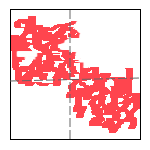
\includegraphics[width=\textwidth]{quadtree_exA.png}
        \caption{Target regions selected by \textit{Analyst} \\ (more efficient, lower reward)}    
        \label{fig:quadtree_a}
    \end{subfigure}
    \hfill
    \begin{subfigure}[b]{0.475\textwidth}  
        \centering 
        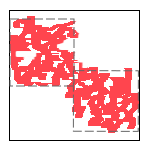
\includegraphics[width=\textwidth]{quadtree_exB.png}
        \caption{Target regions selected manually \\ (less efficient, higher reward)}   
        \label{fig:quadtree_b}
    \end{subfigure}
    \caption[Quadtree algorithm: efficient but sub-optimal.]{\textit{Analyst}'s efficient quadtree results and a higher-reward manual target region selection.}
    \label{fig:quadtree_compare}
\end{figure}
%%%%%%%%%%%%%%%%%%%%%%%%%%
% End quadtree example %
%%%%%%%%%%%%%%%%%%%%%%%%%%

\section{Contributions}
\label{section:contributions}

This research has explored the problem of USV autonomy through the development of two collaborating autonomous agents: an \textit{Analyst} and \textit{Surveyor}. The \textit{Analyst} uses (simulated) aerial images to assign a reward value to each cell in a grid that represents the region that the USV explores. The \textit{Analyst} then uses the reward grid to find regions that offer a high ratio of reward over area and that facilitate efficient coverage. The \textit{Surveyor} generates mission plans that visit as many targets as possible, given constraints on the maximum duration and work. Also, the missions take advantage of opportunities where paths can be made to collect additional reward while remaining feasible. Using the system composed of these agents, the research has posed and investigated several research questions as follows. A major contribution of this work is the development of a modular framework for \textit{Analyst} and \textit{Surveyor} agents so that a variety of techniques can be inserted and evaluated. A second contribution is the implementation of a fitness function for metaheuristic path planning that incorporates dynamic water currents for work minimization as well as the reward grid for reward maximization. The other contributions are the answers to these questions, as will be discussed in the results. 

\begin{itemize}
    \item When using metaheuristic algorithms for \textit{Goto} planning, it has to consider obstacle avoidance, duration minimization, work minimization, and reward maximization. Reward maximization may be opposed to the duration and work minimization. Do the results shown acceptable convergence and repeatibility?

    \item Numerous metaheuristic algorithms exist and have been applied to path planning, though typically only minimizing distance and collisions: particle swarm optimization, genetic algorithm, differential evolution, and artificial bee colony. Which of these is best suited to path planning under these conditions?

    \item Can the weights on the significance of work and reward criteria be set to influence the \textit{Goto} path planning toward a desired path behavior? And are the weights that achieve this behavior transferable across multiple situations since it not reasonable to tune them for each path planning task. 

    \item The presence of water currents impact both the \textit{Surveyor} and \textit{Navigator} of a USV. A forecast of water currents is expected to impact mission planning, but does periodic updating of the water currents appreciably affect the estimated work? 
    
    \item The disadvantage to planning in segments is that each segment is dependent on previous segments, as will be discussed. Instead of evaluating every possible situation, can certain dependencies be ignored and still achieve effective mission planning?
    
\end{itemize}

\section{Prior Work}

Much of the early work in USV research was initiated during WWII by the U.S. Navy, who remains a key player in USV development \cite{bertram2008unmanned}. Military applications include mine-detection, reconnaissance, harbor security, and test targets. Significant growth in USV technology began in the 1990s by the U.S. Navy and continues to this day. A multitude of USVs have been developed outside the military, in academia, commercial, and government sectors \cite{manley2008unmanned} for successful applications in ocean floor mapping, scientific sampling \cite{cokelet2015use}, inspection of industrial platforms, and disaster response \cite{murphy2009robot}. The focus of the proposed research is scientific applications such as benthic mapping and sample collection. While recent advancements in naval USV technology include increasing the autonomy, the scientific use of USVs rarely extends past basic waypoint following or area coverage. The larger goal of this research is mission planning for scientific USV applications, but the target region of interest for this research is narrower. This research is partially motivated by the need to explore the shallow waters along the Texas coast, including inshore bays and lagoons. These regions are of major interest to the local scientific community and it is hoped that the USV and mission planning system developed for this research can be used for practical work in this field. 

As remote sensing systems continue to reduce the human effort in data collection, there is great potential for USVs in oceanographic and marine science applications. A selection of recent examples are as follows. A USV with a sidescan sonar was used in \cite{klemens2017development} for mapping eelgrass in Southern California. A bathymetric map of a lake bed was generated by a USV in \cite{watanabe2016field}. The next example in particular demonstrates the unique character of a USV. The water surface is an air/water interface and is a habitat of specific scientific interest; this region is exactly the operating domain of a USV. A mission is described in \cite{powers2017mobile} where surface temperatures were sampled to produce a high resolution temperature profile of the air/water interface. These example are among many that suggest the growing interest in USVs for scientific applications. 

While numerous successful USV missions have been demonstrated, they have not seen the widespread acceptance of ground and aerial robots. There are several open research problems that impede the proliferation of USVs \cite{bertram2008unmanned, liu:2016}. It is important to remain in contact with deployed USVs in order to make effective use of the remote presence and to respond to emergency situations. The significant cost of over-the-horizon communications for extended USV range is prohibitive to most non-military users. Another issue the logistic complexity of USV deployment and recovery. All but the most shallow-hulled vessels have to exert caution near the shore; some coastal environments may require tedious protocols for deployment of the vehicles. For some tasks, users may find that it is easier to simply use a manned boat or even wade if appropriate. The marine environment is highly corrosive, obstacle-ridden, and subject to sudden and dramatic changes in sea state; these and other factors put USVs at risk and demand reliable and seaworthy vehicles that can survive numerous missions in order to be worth the monetary and logistic cost. There is also a lack of suitable protocols governing USVs that define how they interact with other marine traffic \cite{manley2008unmanned}. Each USV is a stand-alone system whose behavior cannot be reliably predicted by other autonomous vehicles or human ship operators. Finally, the lack of sophisticated autonomy is a major barrier to USV progress. As with other robot modalities, significant attention has been given to autonomous path following control, obstacle detection and avoidance, and path planning. Current USV autonomous systems are largely behavior based and have limited onboard mission planning \cite{liu:2016}. Instead, the USVs either perform simple, tedious jobs or are very human-directed \cite{manley2008unmanned}. For example, in a typical survey mission, a USV is given either a set of human-input waypoints or a search region. The USV executes this mission and returns to base where data is then processed offline. Humans are highly involved in all stages of mission execution: setting goals, verifying progress, processing and evaluating results, and re-deploying the vehicle if needed. The vehicle itself has autonomy for mission execution, but mission planning is almost entirely driven by humans. The vehicle is blind in the sense that it executes the mission, but does not consider the safety and feasibility. 

The lack of onboard mission planning severely limits the potential of USVs. It is desirable to have USVs in operation that can be given generic science goals, and that can use local perception, external data sources, and planning algorithms to achieve these goals with minimal human guidance. This is particularly challenging for marine craft as they are subject to dynamic wind and current forces, sudden weather events, tide fluctuation, other water traffic, and obstacles above and below the water surface. These and other factors of the marine environment must be taken into consideration to ensure efficient mission success as well as safety of the vehicle and marine traffic in its vicinity. Some aspects, such as navigational safety and energy efficiency, are largely independent of the autonomous mission. 

Several schemes have been proposed for classification of levels of autonomy in unmanned systems. One such classification scheme describes eleven levels that range from non-autonomous remote control at level 0 to a fully autonomous vehicle at level 10. In a 2017 review of the current state of USV autonomy, the authors conclude that the current overall level of autonomy for USVs is either level 3 or 4 \cite{heo2017case}. According to their classification system, this means that autonomy can be reliably deployed for real-time collision avoidance, detection of environmental changes, and reaction to those changes. The researchers predict that level 10 is decades away. The authors develop a basic set of requirements for a mission planning system suitable for a USV. These can be broadly summarized as two components. First, the USV should be able to assign goals based on available resources. Second, mission re-planning should be performed in reaction to unexpected situations. 

While little research has been done to develop an integrated high-autonomy USV for scientific applications, some progress has been made in military systems. CARACaS is a state-of-the art mission planning system developed by the U.S. Navy for a swarm of unmanned surface vehicles \cite{heo2017case}. This system integrates the vehicle's sensors and software for dynamic mission planning based on the robot's online perception. The major features of the system are as follows. Static obstacles can be detected and avoided. Resources such as available energy are considered when mission planning. Navigation follows COLREGS regulations; these are traffic rules used to avoid collisions between marine vehicles. COLREGS-based navigation has been explored by other researchers, such as in \cite{naeem2012colregs} where the USV always avoided other vehicles by turning starboard. By following these conventions, other boaters following COLREGS are able to coexist safely with the USV. The system also recognizes threats and can adjust the mission to avoid or to pursue foes. CARACaS has a set of basic mission behaviors that can be initiated depending on the situation and goals, such as patrolling an area, tracking targets, monitoring target activity to determine if they pose a threat, and following targets that have been deemed to be suspicious \cite{wolf2017caracas}. Experimental results demonstrated that a fleet of USVs were able to effectively execute multiple tasks over time without human intervention. 

An important step toward greater autonomy, CARACaS demonstrates a high level of adaptive mission planning. However, the system is focused on military application. The current research seeks to develop a system that enables such autonomy for scientific survey and sampling missions. In addition, there are aspects of mission planning that humans routinely rely upon that is not addressed by the mission planning requirements suggested by \cite{heo2017case}. They discuss the importance of maintaining continuous, high resolution perception for onboard detection and response to events. But the use of external updates and forecasts of future events is not addressed, which is a basic component of human mission planning. Consider this situation where a science team is planning to use a boat, whether manned or unmanned, to map some area. In advance, they would be checking the weather to ensure that is reasonable to do so. Even if the boat is robust and not in any danger during, for example, a light storm, the weather conditions could strongly impact the quality of data. An autonomous "science agent" should have some capability to access weather predictions to plan missions that consider both vehicle safety and data quality. It can be argued that accessing these resources will be difficult for a USV where robust communication is still an active research topic. However, the requirement that robots should be continually monitored in order to react to emergencies necessitates that suitable communication exists. 

\chapter{System Design}

A system is created that implements the \textit{Analyst} and \textit{Surveyor} to study underwater \textit{entities}, such as types of seagrasses. The system so far is entirely within simulation. The region and water currents forecasts are taken from real-world data sources, but the entities are simulated as will be described. An overview of the system is shown in \ref{fig:system_overview}. The system made up of a number of separate modules, most of which may be run independently. For example, a particular path planner module may be used as a stand-alone program rather than as a part of a larger mission planning program. Similarly, other path planners can be introduced and chosen selectively. Each of the three intelligent agents previously described are represented by sets of system modules. The \textit{Analyst} has programs and utilities for determining the reward, \textit{interestingness} of specific targets or cells in the environment's grid representation. It can generate a set of target regions for \textit{Coverage} tasks that will be given to the \textit{Surveyor} as mission planning goals. The mission generated by the \textit{Surveyor} is then used by the \textit{Navigator} who handles the onboard following of the plan as specific motor commands for the robot. This focus here is on the \textit{Surveyor}'s mission planning since it has been given most attention with results available for meaningful analysis. The \textit{Analyst}'s programs and results will be discussed, but less analysis is done since it currently works with simulated data and its optimality is difficult to define.

\begin{figure}[H]
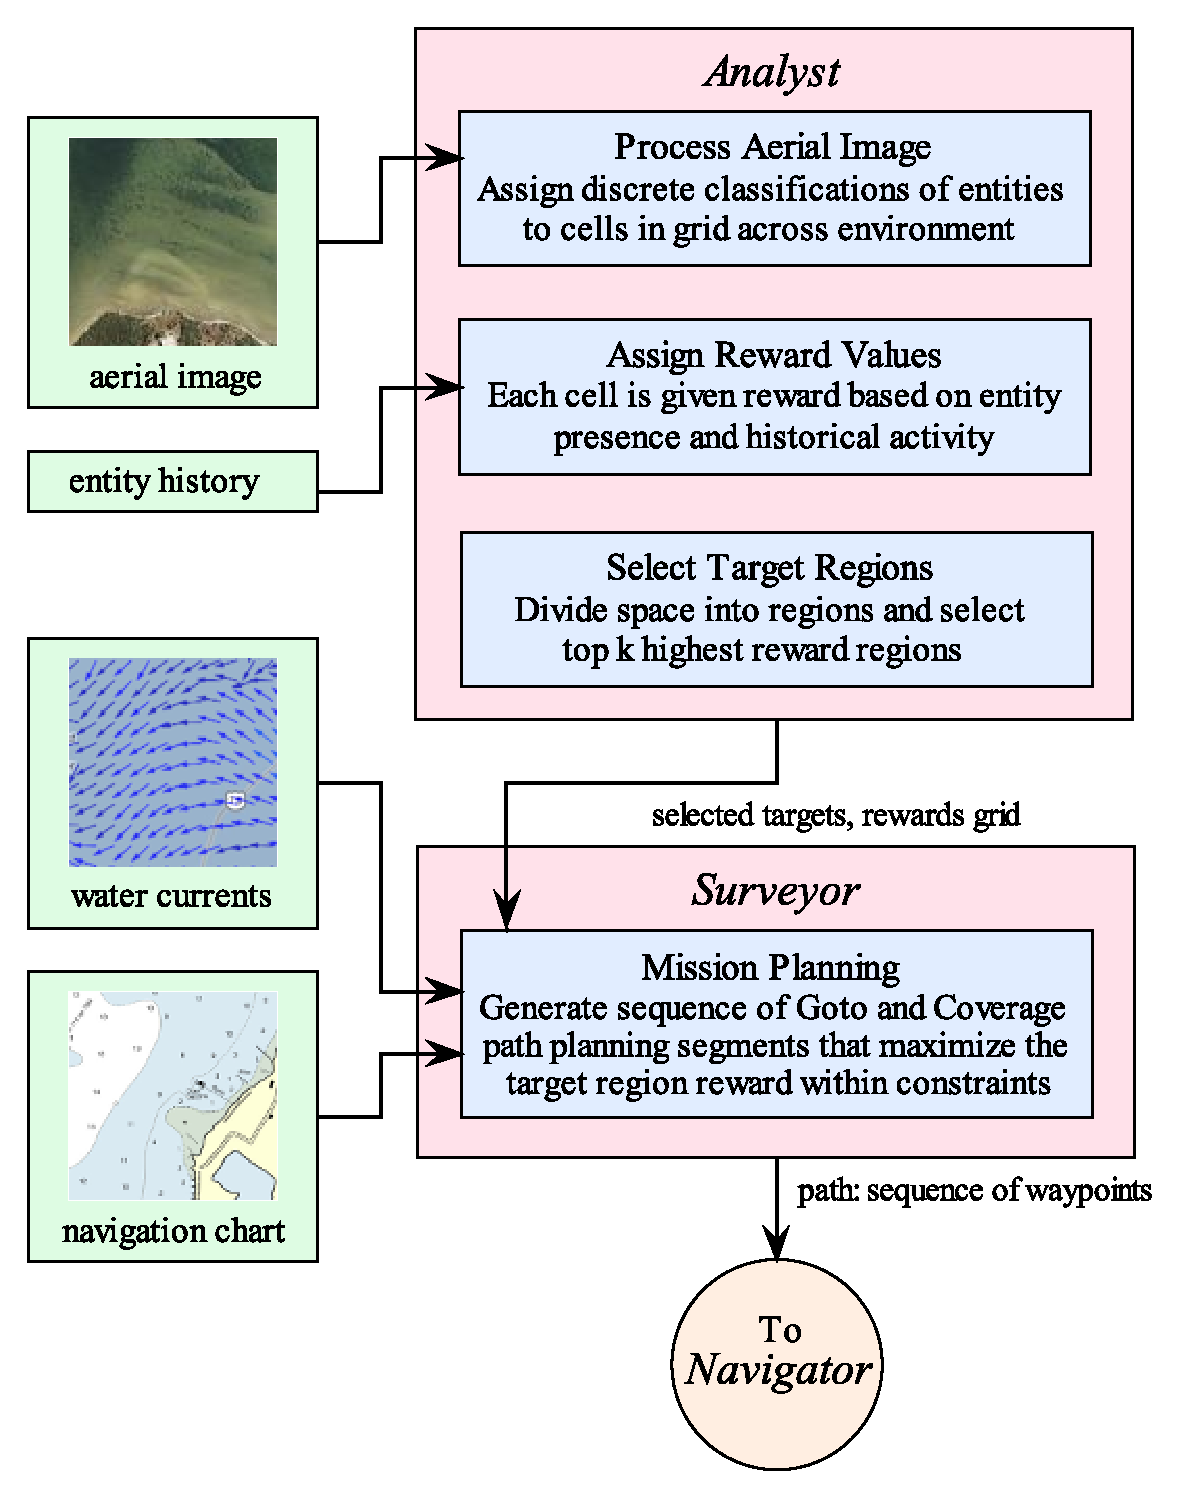
\includegraphics[width=\textwidth]{system_overview.eps}
\caption[System as the collaboration of multiple autonomous agents.]{System as the collaboration of multiple autonomous agents.}
\label{fig:system_overview}
\end{figure}

\section{\textit{Analyst} Agent}

The \textit{Analyst} is not applied to a specific real-world problem, but rather demonstrates the role's concept using simulated data. The data is a sequence of images, where each color in the image represents an entity and so each cell is associated with a single entity. A completely white cell indicates the absence of an entity, and a black cell indicates that the value is unknown. Only the red value is used for entity assignment, which limits the number of possible entities to 255. The other color values could later be used to represent additional information such as certainty of the identification. (HSV could be used to more intuitively communicate the purpose of the color values; ie: a lower saturated pixel representing less certainty). Since the \textit{Analyst} needs to assign reward values to all cells in the world representation's grid, an image is a reasonable method for storing entity information. A sequence of images is given to the \textit{Analyst}, where each image represents a snapshot of the entities at a particular time. A cellular automata is used to perturb the image by adding and removing pixels based on growth and decay rates of each entity type. There are also randomly generated events such as a sudden appearance of some pattern; these represent anomalies that should be noticed by the \textit{Analyst}. The author of this work has previously done work where a USV performed online detection of seagrass using an RGB camera. The output is an image where each pixels's color is code for either \textit{seagrass}, \textit{not seagrass}, \textit{unsure}, or \textit{unchecked}. This is an example of real-life data that could be used. The simulated data was used since there is a lack of historical imagery, which is used in the procedure described below. 

This example \textit{Analyst} employs a simple method of reward assignment. The key points is that it uses both the most recent image as well as recent history in its calculation. Each entity has a weight listed in a table. Here, the table was manually created since the scenario is entirely fabricated. With a sufficiently large history of images, entities could be generated from unsupervised learning and their weight based on some scientific criteria. However, it is assumed that for this example it is either the case that such automatic assessment has taken place or the weights are informed by an expert. There is no requirement that the \textit{Analyst} is not given some initial human-input information about its environment and goals. It just has to be capable, as a baseline, of automatic reward assignment and target selection. 

The entire environment is segmented into blocks where each block contains a number of cells. The density of entities in each block is used to add reward to each cell in the block. Thus, cells nearby to entities get some reward, proportional to the total strength of weighted entities in that block. The idea is that if the imagery observes something interesting, the area surrounding is also interesting since it may contain unobserved entities or have characteristics that help explain the entities presence. Next, the speed and acceleration of entity growth or decay within that block is calculated and used to add additional reward to the cells. The importance of speed and acceleration of each entity type has its own weight: some entities may have been observed to be fast and this is not interesting. The \textit{Analyst} records and outputs a separate grid of the reward for each entity type. The total reward of a cell is the summation of the reward in all grids at that cell. 

In addition to sharing the reward grids with the \textit{Surveyor}, the \textit{Analyst} uses them to generate target regions intended to be used in \textit{Coverage} planning. 

The quadtree algorithm is used to partition the reward grid such that each partition is a potential target region. Quadtree recursively divides the grid into subgrids until one of the base cases is reached. The specification of base cases controls the characteristics of the resulting coverage regions available to choose from as targets. Because of both planning complexity and the time it takes to physically traverse a region, an upper limit, $L_u$, is placed on the partition size, $P_n$. Since planning and executing terrain-free region coverage is trivial, terrain-free regions are allowed to stop at $L_u$ if the partitions meet other requirements. A terrain-free region of allowed size may be insufficient reward to make a desirable target region. Either a reward threshold, $T_r$, or percentage of cells containing entities, $T_e$, should be met before stopping only based on $L_u$. Both or only one of the criteria may be enabled. 
Incorporating these criteria, base case (1) is terrain-free, $P_n \leq L_u$, and either the total reward is $\geq T_r$ or proportion of cells with entities is $\geq T_e$. This base case yields terrain-free target regions of desired size and reward or entity presence. A lower limit, $L_l$, defines the smallest allowed regions. Regions with terrain should be kept small since \textit{Coverage} planning complexity increases exponentially with additional cells in regions with terrain. Base case (2) is when $P_n \leq L_l$. Because of the smaller size, regions with terrain are only selected if they have large reward relative to other regions. It is possible to reach the lower limit with terrain-free regions because of insufficient reward. A final base case, (3), is included only to reduce unneeded recursion. If the proportion of cells with terrain exceeds a maximum, $O_n$, then the obstacle-dense region does not need to be divided further. 

While the intention is to present an abstract methodology, the \textit{Analyst} was developed with seagrass studies in mind. Sudden patterns of loss are likely indicators of seagrass bed scarring or other source of damage. Thus, the speed and acceleration of loss can guide the vehicle to investigate. There are also "no fast" seagrasses, so sudden growth would warrant attention. This mentioned is to clarify some of the choices made and to suggest that there is not a single solution to the \textit{Analyst} implementation. 

\section{\textit{Surveyor} Agent}

\subsection{Environmental Representation}

A finite rectangular region is selected as the robot's exploration domain and is divided into a discrete grid of equally sized cells. The resolution impacts the planning quality in two ways. If the cellsize exceeds the diameter of the sensor, then the path planner's coverage estimation differs from reality. Second, more accurate distance, duration, work, and reward estimates are achieved at higher resolutions. Multiple grids are used to represent different characteristics of the environment. The grids used by the \textit{Surveyor} implemented in this system are listed in Table \ref{tbl:grids}. 

\begin{table}[H]\small
\begin{tabular}{|l|l|}
\hline
Grid            & Description \\
\hline
$G_{region}$    & Binary occupancy grid where 0 indicates free (water) and 1 indicates occupied (terrain) \\
\hline
$G_{magnitude}$ & Cell values are the water current forecast's magnitude for that location \\
\hline
$G_{direction}$ & Cell values are the water current forecast's direction for that location \\
\hline
$G_{reward}$    & Cell values are the reward for that location, as determined by the \textit{Analyst} \\    
\hline
\end{tabular}
\caption{Descriptions of grids used by the \textit{Surveyor} to represent the environment.}
\label{tbl:grids}
\end{table}


\section{Path Planning}

Path planning forms the building blocks of mission planning, so is presented first. Characteristics of path planning, such as its limitations and dependencies, motivate various choices in the mission planner design. Two types of path planner are discussed and an implementation of both exists in the system and are used in mission planning.

\subsection{Goto Path Planner} \label{section:goto}

The \textit{Goto} planning module is responsible for generating point-to-point paths between a start and stop location. The module is used by the mission planners to plan mission segments between nodes (targets, start, and stop locations). Due to the complexity of path planning (NP-hard), heuristic and meta-heuristic algorithms have become standard over optimal methods such as breadth-first search which enumerates all possible paths. Because the scientific missions are expected to operate over very large areas, the search space will be massive. This motivates the emphasis on meta-heuristic algorithms that dramatically reduce the search space at the expense of some optimality. The experiments in this text use a 1000x1093 grid which is very large for planning, and could still be called low resolution for the 229,622,675 $m^2$ region. The actual grid size for real missions should be such that the sensor covers a cell entirely if complete coverage is required. Meta-heuristic path planning is well-established to give approximately optimal results in point-to-point planning that minimizes distance, duration and avoids obstacles \cite{hussein2012}. Rather than repeat this known result, the investigation here focuses on a comparison of algorithms and the effect of including the criteria of minimizing work and maximizing reward. Does one algorithm perform better than the others and is this affected by the addition of work and reward optimization? Can the weights be manipulated to achieved a desired planning behavior that is reliable across multiple situations? Four common meta-heuristic algorithms are compared to select the best to be the \textit{Goto} planner's default algorithm: Genetic Algorithm (GA), Differential Evolution (DE), Particle Swarm Optimization (PSO), and Artificial Bee Colony (BEE). All four are implemented using the PyGMO optimization library \cite{PyGMO}. Path attributes (distance, duration and work) are measured with respect the the cells rather than the actual distance. They should be converted appropriately for field use. In all four cases, PyGMO's default parameters are used. Additional work could be done to tune these further, but the defaults are ones that have been observed to be generally effective, and tuning has the possibility of overfitting for the specific tasks used in the experiments. 

\subsubsection{Genetic Algorithm}

GA is based on the evolutionary concept of natural selection to iteratively evolve toward an optimal solution \cite{ga:cao:2016}. The core of GA is that survival of the fittest is used to transform a population of individuals, each a potential solution, into another population with higher average fitness. After evolution proceeds for some time, the fitness should become stable: the fitness of the population is approximately (possibly local) optimum and receive little or no benefit from additional iterations. The individual with highest fitness is chosen as the problem solution. The mechanisms behind GA are the selection, mutation, and crossover operations. Selection is process of choosing which individual's solutions are to be used for constructing the next generation. Individuals are ranked by their fitness and the probability of selection is proportional to the individual's fitness. New individuals are formed from those selected using crossover and mutation. The crossover operation combines elements of solutions (called genes) in combination, with the hope that elements from two fit solutions can be combined to yield an even better solution. While not all of these combinations will have better fitness, the selection process will favor the better results: guiding the population in increasingly fitter solutions on average. Mutation is the operation of randomly adding, deleting, and transforming genes. Many mutations will be harmful, but again, selection will promote the survival of those that improve the population. The result of GA is sensitive to the rate of mutation and crossover. An overemphasis on crossover may lead to premature convergence to an optimal solution, since the space is insufficiently explores. But an overemphasis of mutation may not take advantage of fit solutions and delay convergence. The parameters (PyGMO defaults) are as follows. \textit{Selection} is set to \textit{tournament}, \textit{crossover strategy} to \textit{exponential}, \textit{crossover probability} to \textit{0.9}, \textit{mutation strategy} to \textit{polynomial}, \textit{mutation probability} to \textit{0.02}. 

% % --------------------  Genetic Algorithm --------------      
% \begin{algorithm}[H]
% \KwIn{population size $P$, \\
% ~~~~~~number of iterations $N$, \\
% ~~~~~~mutation rate $M$, \\
% ~~~~~~crossover rate $C$, \\
% }
% \KwOut{Solution $X$}
% \textbf{begin GA}\\
% ~~~Randomly initialize a population of $P$ individuals\\
% ~~~Set iteration counter $c$ = 0 \\
% ~~~\textbf{While} (While $c$ is less than $I$) do\\
% ~~~~~~~~~~~\textbf{For} i = 1 to number of individuals \\
%  ~~~~~~~~~~~~~Evaluate the fitness:= $ f(x_i)$\\
%  ~~~~~~~~~~~~~Select individuals with probability proportional to their fitness \\
%  ~~~~~~~~~~~~~Apply crossover to selected individuals with probability $C$\\
%  ~~~~~~~~~~~~~Apply mutation to selected individuals with probability $M$ \\
%  ~~~~~~~~~~~~~Set the current solution $X$ as the fittest individual \\
%  ~~~~~~~~~~~~~Set the population as the resulting generation from application of the genetic operations\\
% ~~~\textbf{End while} \\
% \textbf{end GA}\\
% \caption[Basic steps of genetic algorithm.]{Basic steps of genetic algorithm.}
% \label{GA}
% \end{algorithm}
% % ----------------- End Genetic Algorithm --------------

\subsubsection{Particle Swarm Optimization}

PSO differs conceptually from GA in that it deals with activity within a single, static population, rather than its evolution \cite{pso:nie:2016}. The algorithm models a group of social particle, each a solution, that share information to locate resources. They search for resources within the problem's search space, using a fitness function to determine which points offer better resources. Particle are characterized by their positions (solutions), its personal best solution, and its velocity. Each also has access to it's neighborhood's best solution where the neighborhood is the 4 solutions stored adjacent in the population array. At every iteration, particle move in the search space with a velocity influenced by the global and local information. The parameters (PyGMO defaults) are as follows. \textit{Inertia weight} is set to \textit{0.7298}, \textit{social weight} to \textit{2.05}, \textit{cognitive weight} to \textit{2.05}, \textit{maximum velocity} to \textit{0.5}, \textit{neighborhood} (swarm topology) to \textit{immediate solutions in population array}, and \textit{neighborhood size} (topology parameter) to \textit{4}. 

% % -------------------- PSO algorithm --------------      
% \begin{algorithm}[H]
% \KwIn{population size $P$, \\
% ~~~~~~number of iterations $N$, \\
% }
% \KwOut{Solution $X$}
% \textbf{Begin PSO}\\
% ~~~Randomly initialize the position and velocity of the $P$ particles: $X_i(0) and V_i(0)$\\
% ~~~Set iteration counter $c$ = 0 \\
% ~~~\textbf{While} (While $c$ is less than $I$) do\\
% ~~~~~~~\textbf{For} $i$ = 1 to number of particles \\
%  ~~~~~~~~~~Evaluate the fitness:= $ f(x_i)$\\
%  ~~~~~~~~~~Update local and global best solutions \\ 
%  ~~~~~~~~~~Update velocity of the particle $v_i$\\
%  ~~~~~~~~~~Update position of the particle $x_i$\\
%  ~~~~~~~~~~Compute fitness of new population\\
% ~~~\textbf{End while} \\
% ~~~Set the solution $X$ using the fittest individual \\
% \textbf{end PSO}\\
% \caption[Basic steps of particle swarm optimization.]{Basic steps of particle swarm optimization.} 
% \label{PSO}
% \end{algorithm}
% %----------------- End PSO algorithm ---------------

\subsubsection{Differential Evolution }

DE is similar in concept to GA, but the mechanics of population improvement differ \cite{de:zhang:2013}. Rather than using separate mutation and crossover operations, a single manipulation function exists that incorporates aspects of both. The function takes three individuals in the population and computes a new value as a combination of the three inputs. The critical piece of the function is a difference between solution elements so that the change is more strongly influenced by further apart individuals. Since this function creates new solution elements, but based on elements found in the existing population, it can be thought of as a crossover-driven mutation operation. The behavior is controlled with a crossover rate $C$ that affects how often the operation is applied and a differential weight $F$ which affects how strongly the vector differences can influence a candidate. The concerns regarding premature or delayed convergence in GA remain. The parameters (PyGMO defaults) are as follows. The \textit{weight coefficient} is set to \textit{0.8}, the \textit{crossover probability} to \textit{0.9}, and \textit{mutation algorithm} set to \textit{rand/1/bin} (\cite{de:neri:2010}). 

% % -------------------- DE algorithm -------------- 
% \begin{algorithm}[H]
% \KwIn{population size $P$, \\
% ~~~~~~number of iterations $N$, \\
% ~~~~~~crossover rate $C$ \\
% ~~~~~~differential weight $F$ \\
% }
% \KwOut{Solution $X$}
% \textbf{Begin DE}\\
% ~~~Randomly initialize the position of the $P$ agents\\
% ~~~Set iteration counter $c$ = 0 \\
% ~~~\textbf{While} (While $c$ is less than $I$) do\\
% ~~~~~\textbf{For} each agent $x$ \\
% ~~~~~~~Randomly select 3 distinct agents, $a$, $b$, $c$ that are not $x$ \\
% ~~~~~~~Randomly select a solution element (vector index $i$) \\
% ~~~~~~~Initialize a new vector $y$ of the length of the solution dimension. Each element is $0$. \\
% ~~~~~~~\textbf{For} $i$ = 0 to length of solution \\
% ~~~~~~~~~Randomly select $r_i$ from uniform distribution in range $[0, 1]$ \\
% ~~~~~~~~~\textbf{If} $r_i$ < $C$ \\
% ~~~~~~~~~~~Set $y_i$ = $a_i + F * (b_i - c_i)$ \\
% ~~~~~~~~~\textbf{Else} \\
% ~~~~~~~~~~~$y_i$ = $x_i$ \\
% ~~~~~~~~~\textbf{If} candidate solution $y$ has greater fitness than $x$ \\
% ~~~~~~~~~~~Replace agent $x$ with improved agent $y$ \\
% ~~~\textbf{End while} \\
% ~~~ Set $X$ as solution with greatest fitness \\
% \textbf{end DE}\\
% \caption[Basic steps of differential evolution.]{Basic steps of differential evolution.}
% \label{DE}
% \end{algorithm}
% % ----------------- End DE algorithm -------------- 

\subsubsection{Artificial Bee Colony}

ABC is similar to PSO in that the individuals in the population search for the solution by performing actions \cite{bee_ga:carballo:2017}. The bees are searching for food (solutions) with a high quantity of nectar (fitness). Like bees in nature, the individuals fulfill different role and may go between roles depending on the situation. The roles are employed, onlookers, and scouts. The population is food sources which represent solutions. The number of employed bees is equal to the number of solutions such that every employed bee is associated with a single solution. Initially, food sources are randomly generated in the search space. At each iteration, there are distinct phases for the activity of employed, onlooker and scout bees. Employed bees search the neighborhood of their food source to check for better food nearby sources. The bee checks an adjacent location and updates the food source if the fitness is higher than the current source. Note that the bee is, in a single iteration, only checking one solution in the neighborhood: a greedy search. So, an employed bee either maintains or replaces the food source at each iteration. After this, the onlooker bees select sources from those offered by the employed. This selection is done with the consideration of each solution's fitness. The fitness is used to weight the probability of choosing that source. The onlooker, like the employed bee, looks at nearby solutions in search of fitter sources. If the location checks has higher fitness, the onlooker records the solution and its fitness. The scouts randomly find new solutions to replace existing solutions. Solutions are abandoned when a set number of iterations goes by without finding a higher reward that the current solution. The employed bee that abandons its source temporarily becomes a scout in order to find new sources. The onlookers contribute to convergence by searching around known solutions, while the scouts promote exploration by randomly checking new solutions.  The parameters (PyGMO defaults) are as follows. The \textit{limit}, which is the number of iterations before an employed bee abandons a food source when unable to increase fitness, is set to \textit{1}. 

% % -------------------- BEE algorithm -------------- 
% \begin{algorithm}[H]
% \KwIn{population size $P$, \\
% ~~~~~~number of iterations $N$, \\
% ~~~~~~limit $L$ \\
% }
% \KwOut{Solution $X$}
% \textbf{Begin BEE}\\
% ~~~Randomly initialize position of the employed bees \\
% ~~~\textbf{For} $e$ in employed bees \\
% ~~~~~~~\textbf{For} $n$ in solution neighborhood \\
% ~~~~~~~~~Calculate fitness of solution $n$ \\
% ~~~~~~~~~\textbf{If} fitness of $n$ > fitness of current solution \\
% ~~~~~~~~~~~~~Set solution to $n$ \\
% ~~~~~~~\textbf{If} bee has been unable to improve fitness for $L$ iterations \\
% ~~~~~~~~~~~Switch to scout bee \\
% ~~~~~~~Use selection scheme to select an employed bee's solution \\
% ~~~~~~~\textbf{For} $n$ in solution neighborhood \\
% ~~~~~~~~~Calculate fitness of solution $n$ \\
% ~~~~~~~~~\textbf{If} fitness of $n$ > fitness of current solution \\
% ~~~~~~~~~~~~~Set solution to $n$ \\
% ~~~\textbf{For} $s$ in scout bees \\
% ~~~~~~~Randomly choose a now solution \\
% ~~~~~~~Switch to employed bee \\
% ~~~Record best solution found by all bees so far as $X$ \\
% \textbf{end BEE}\\
% \caption[Basic steps of artificial bee colony.]{Basic steps of artificial bee colony.} 
% \label{BEE}
% \end{algorithm}
% % ----------------- End BEE algorithm -------------- 

\subsubsection{Fitness Function}
\label{section:fitness_function}

A solution path is presented as a sequence of waypoints, demonstrated in Equation \ref{solution_path}. Each element is a tuple with an x and y coordinate into the environment grid. 

\begin{equation}
path = [ (x_{1}, y_{1}), (x_{2}, y_{2}), ..., (x_{n}, y_{n}) ]
\label{solution_path}
\end{equation}

The fitness function evaluates the quality of a candidate solution; each metaheuristic algorithm employs some scheme to optimize the fitness value. In this system, the \textit{Surveyor} intends to minimize collisions, distance, duration, and work. Duration is not calculated in the fitness function since it related to the distance and work. This is complicated by that the \textit{Surveyor} also intends to sacrifice some optimality to maximize path reward. Weights are used to influence the importance of each criteria. High weight on reward should cause the \textit{Surveyor} to be less concerned with path efficiency, while a very small (or 0) reward weight focuses only highly efficient planning. The path distance, $Path_D$, (equation \ref{eq_path_distance}) is the sum of euclidean distances between each pair of adjacent waypoints, $(x_{i}, y_{i})$ and $(x_{i+1}, y_{i+1})$. The path obstacles, $Path_O$, is the count of all collisions between each pair of waypoints (equation \ref{eq_path_obstacles}). The work exerted by the vehicle, $Path_W$, is the sum of work done along the path segments as it deals with water currents to maintain a constant speed (equation \ref{eq_path_work}). Note that equation \ref{eq_work_prime} is a call to Algorithm \ref{alg:getworkatcell}. Finally, the reward collected by visiting cells along the path, $Path_R$, is the sum of reward values in $G_{reward}$ (equation \ref{eq_path_reward}). The calculations of $Path_O$, $Path_W$, and $Path_reward$ require checking all cells in a line between the two adjacent paypoints. The Bresenham line algorithm \ref{bresenham:1965} gives the set of all grid cells between any two grid points. The fitness for the entire path is the weighted sum of these values, using weights $W_{distance}$, $W_{obstacles}$, $W_{work}$, and $W_{reward}$ (see Equation \ref{fitness_function}). The weight $W_{obstacles}$ is always set to an arbitrary large number, since there are no situations where the \textit{Surveyor} allows collision. 

% --- Distance Eqs ---
\begin{equation}
\Delta (x_{i}, y_{i}, x_{j}, y_{j}) = \sqrt{(x_{i} - x_{j})^2 + (y_{i} - y_{j})^2}
\label{eq_distance}
\end{equation}

\begin{equation}
Path_{D} = \sum_{i=1}^{n-1} \Delta (x_{i}, y_{i}, x_{i+1}, y_{i+1}) \forall (x_{i}, y_{i}) \in (x_{1}, y_{1}), (x_{2}, y_{2}), ..., (x_{n-1}, y_{n-1})
\label{eq_path_distance}
\end{equation}
% - End  Distance Eqs --


% ---- Obstacle Eqs ----
\begin{equation}
o = \sum G_{region}(x_l, y_l) \forall x_l, y_l \in Bresenham(x_i, y_i, x_j, y_j) 
\label{eq_obstacles}
\end{equation}

\begin{equation}
Path_{O} = \sum_{i=1}^{n-1} o (x_{i}, y_{i}, x_{i+1}, y_{i+1}) \forall (x_{i}, y_{i}) \in (x_{1}, y_{1}), (x_{2}, y_{2}), ..., (x_{n-1}, y_{n-1})
\label{eq_path_obstacles}
\end{equation}
% - End Obstacle Eqs ---

% ---- Work Eqs -----
\begin{equation}
\omega^{'} = GetWorkAtCell(x_l, y_l), 
\label{eq_work_prime}
\end{equation}

\begin{equation}
\omega = \sum \omega^{'}(x_l, y_l) \forall x_l, y_l \in Bresenham(x_i, y_i, x_j, y_j) 
\label{eq_work}
\end{equation}

\begin{equation}
Path_{W} = \sum_{i=1}^{n-1} \omega (x_{i}, y_{i}, x_{i+1}, y_{i+1}) \forall (x_{i}, y_{i}) \in (x_{1}, y_{1}), (x_{2}, y_{2}), ..., (x_{n-1}, y_{n-1})
\label{eq_path_work}
\end{equation}
% - End work eqs ----

% ---- Reward Eqs -----
\begin{equation}
\gamma = \sum G_{reward}[(x_l, y_l)] \forall x_l, y_l \in Bresenham(x_i, y_i, x_j, y_j)
\label{eq_reward}
\end{equation}

\begin{equation}
Path_{R} = \sum_{i=1}^{n-1} \gamma (x_{i}, y_{i}, x_{i+1}, y_{i+1}) \forall (x_{i}, y_{i}) \in (x_{1}, y_{1}), (x_{2}, y_{2}), ..., (x_{n-1}, y_{n-1})
\label{eq_path_reward}
\end{equation}
% - End reward eqs ----


% ----- Combined fitness function -----
\begin{equation}
\begin{aligned}
Fitness_{path} ={} & \{W_{obstacles} \times Path_{O} + \\ 
                    &  W_{distance} \times Path_{D}  + \\
                    &  W_{work} \times Path_{W}     - \\
                    &  W_{reward} \times Path_{R}\}
\end{aligned}
\label{fitness_function}
\end{equation}


\begin{spacing}{0.5}
% ------------- Get work at cell -------------- 
\begin{algorithm}[H]
\caption[GetWorkAtCell]{\textbf{GetWorkAtCell:} Calculate the work done to traverse a cell} 
\label{alg:getworkatcell}
\SetAlgoVlined
\KwIn{Location coordinates $<R_x, R_y>$, waypoint coordinates $<W_x, W_y>$, desired robot speed $s$, cell size $c$, time offset $d$, grid of environment force magnitudes $Grid_{magnitude}$, and grid of environment force directions $Grid_{direction}$. }
\KwOut{Work estimate $w$}
\If{$d == 0$}{
    $idx = 1$}
\Else{$idx = ceil(d / bandinterval$)}
$\theta_h = angle(<0, 1>, <W_y, W_x>)$\;
$V^r_x = s \times \cos{\theta_h}$\;
$V^r_y = s \times \sin{\theta_h}$\;
$V^e_x = Grid_{magnitude}(idx, R_y, R_x) \times \cos{Grid_{direction}(idx, R_y, R_x)}$\;
$V^e_y = Grid_{magnitude}(idx, R_y, R_x) \times \sin{Grid_{direction}(idx, R_y, R_x)}$\;
$V_{\delta x} = V^r_x - V^e_x$\;
$V_{\delta y} = V^r_y - V^e_y$\;
$\theta_{\delta} = angle(<V_{\delta y}, V_{\delta x}>, <0, 1>)$\;
$s_{\delta} = \sqrt{(x_{i} - x_{j})^2 + (y_{i} - y_{j})^2}$\;
$w = s_{\delta} \times c$\;
\Return {w}
\end{algorithm}
% --------------- Get work at cell -------------- 
\end{spacing}


\subsection{Coverage Path Planner}

\textit{Coverage} path planning is used to find a path that reaches all (or a specified minimum proportion) of cells over a target region. The mechanism of path generation differs greatly from \textit{Goto} planning because of the need to maximize cell coverage. It is a complex problem since the path should visit each cell while still minimizing distance. Every cell added increases the distance, so distance minimization means that the no other path through all cells will be shorter distance. In this system, work and distance are both of concern. Like \textit{Goto} planning, algorithms may be exhaustive, heuristic, or meta-heuristic. 

Because of the large dimension of candidate solutions (from a waypoint-based planning perspective (Equation \ref{solution_path}), efforts to apply metaheuristic algorithms have applied various techniques for search space reduction. These techniques typically make assumptions on the environment are not useful for highly-complex situations. This \textit{Surveyor} is dealing with complex geographic shapes. For this domain, it is better to have less-optimal planners that place few restrictions on the environment. 

The implementation of \textit{Coverage} planning within this system is still in its infancy. Some form was needed to be able to use the mission planner, since each target corresponds to a \textit{Coverage} task. Currently, a simple lawnmower path algorithm is employed for terrain-free regions. Without the need to work around obstacles, planning is trivial. The dynamics of USVs are not suited to the sharp turn inherent in lawnmower paths, which traverse the regions grid in either row-wise or column-wise movements \cite{liu:2016}. Still, the generic nature of lawnmower paths makes them usable by any standard vehicle, and they remain common for USV survey tasks despite their inefficiency. The lawnmower coverage planner implemented computes both row-wise and column-wise paths. The directions of the currents can greatly impact the relative performance of the two schemes, so both are evaluated and the more efficient is selected. 

If a target region has terrain, a metaheurstic planner is invoked. This planner is still under construction and is highly inefficient in its current state. Such regions are not featured in this text. Because the \textit{\textit{Analyst}} selects large and reward-rich terrain-free regions where possible, it was not necessary to manual intervene for the system to naturally select terrain-free targets. In theory, exceptionally rare events or desirable entity presence would lead the \textit{\textit{Analyst}} to select regions with terrain despite their smaller size.


\subsection{Mission Planning}

A mission planner is a program that takes as input a start location and a number of targets and allowed stop locations. The start and stop locations are simply latitude and longitude coordinate points, but the targets have both coordinate and extent. The coordinate is the center of the region and the extent specifies the area of the region around that point. Collectively, the start, stop, and target locations are called nodes. At the highest level, a solution mission is a sequence of nodes that represents a sequence of mission segments. The mission planners used in this research generate a sequence of \textit{Goto} and \textit{Coverage} path planner segments. An example mission, with \textit{Goto} and \textit{Coverage} paths evaluated, is shown is Figure \ref{fig:missionplanning}. 

\begin{figure}[H]
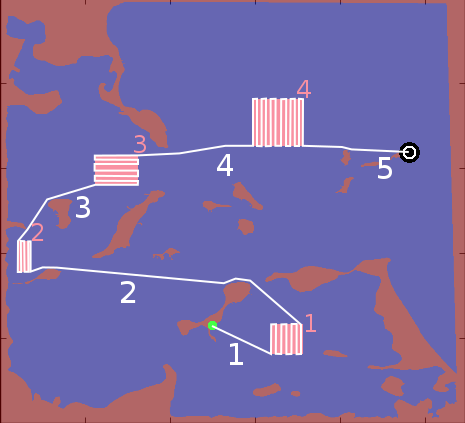
\includegraphics[]{nummissions.png}
\caption[Example mission.]{Example mission. With 4 targets, there are 4 \textit{Coverage} paths and 5 \textit{Goto} paths.}
\label{segment_example}
\end{figure}

The goal of the mission planner is visit as many targets as is feasible and end at one of the allowed stop locations.  The mission planner chooses an optimal order in which to visit the targets. Consider a solution mission $( 0, 2, 1, 3 )$. This represents a \textit{Goto} path from the start location at node 0 to a target region's entry location at node 2. The entry location is a point on the boundary of a target region that is selected as the point to start from when arriving from a specific previous node. In other words, there may be a different entry point into the region of node 2 if the previous node were 1 rather than 0. At node 2, the \textit{Coverage} path is performed by visiting cells in the region and ending at the region's exit location. Similarly to the entry location, the exit location is defined with respect to the next node in the sequence. This is illustrated in Figure \ref{segment_example}. After completing the \textit{Coverage} task, another \textit{Goto} task is followed to reach the entry location for node 1. Again, a \textit{Coverage} task is done followed by a \textit{Goto} to reach the stop at node 3. The output of the mission planner should be a feasible path, which is one whose total duration and work do not exceed the maximum constraints. For example, the robot may have both limited power and a directive to end within 5 hours. The mission planner produces only estimates of feasible paths, but will be considered feasible for the purpose of this analysis. 

Two mission planner programs have been developed and their results will be compared in this text. These are called Mission Planner Fully Connected (MPFC) and Mission Planner Try \& Repair (MPTR), and they largely differ in the number of path planner modules invoked. Ultimately, mission planning reduces to a form of the travelling salesman problem which is NP-hard. Various techniques have been developed to deal with NP-hard problems by reducing the search space with heuristics or meta-heuristic approaches. An example is A* which uses the distance between nodes as a heuristic in deciding which nodes to explore. Meta-heuristic algorithms, such as those used by planning modules in this system, have been demonstrated to achieve very high computational performance in reaching (non-deterministic) approximately optimal solutions. Because this system uses different types of search algorithms in different modules, a distinction needs to be clarified to avoid confusion. Both mission planners invoke path planners for finding specific paths for each mission segment. Only the selection of targets and the order of these segments is handled by the mission planner itself. MPFC is an exhaustive search of all possible paths. The estimated distance, duration, work, and reward is totalled for each possibility and used to select the best feasible mission. This called optimal with respect to all other missions, but cannot be called absolutely optimal with regards to the path since the segments are computed using approximately optimal path planners. Optimal here is intended to convey an ideal mission planning result given the mission planning setup in place. The goal is show that a mission planning scheme can be developed which approximates the result of MPFC, but with less complexity. MPTR ignores two path planning elements that forces sequence planning of segments. The two elements are (1) after each segment, the elapsed duration is input to the next segment so that the current forecast is updated accordingly and (2) the order of nodes determines the entry into and exit from \textit{Coverage} regions. The final mission requires that the both elements are taken into account. However, the question is whether or not a reasonable sequence of nodes could be determined without those elements. In other words, could a mission planner ignore the elements to determine that an effective sequence is nodes $(1 3 4 2 5 6$ and then plan that sequence fully with the elements applied appropriately. If so, MPTR would reduce the mission planning to hours instead of days, in its current form. With further optimization of the fitness function and parallel execution of planner invocations, this is likely to become minutes instead of hours. Both MPFC and MPRT will now be discussed in full.

\subsubsection{Mission Planning Inputs}

The required data files for both mission planners are listed in Table \ref{tbl:planner_input}. The table describes each input file and lists where an example of the file can be found in this text. 

\begin{table}[H]\small
\begin{tabular}{|p{2.75cm}|p{5cm}|l|l|}
\hline
Name & Description & File type & Example in text \\
\hline
System config    & Numerous system parameters  & YaML (plaintext) & Source code \\
\hline
Entities config  & Weights, labels, and color codes for entities  & YaML (plaintext) & Source code  \\
\hline
Targets table    & Targets to include in mission planning & CSV (plaintext)  & Table \ref{tbl:targets} \\
\hline
Safepoints table & Choices of robot end points & CSV (plaintext)  & Table \ref{tbl:safepoints} \\
\hline
Region map       & Occupancy grid where cells are either occupied or free  & Geotiff raster & Figure \ref{fig:env_terrain} \\
\hline
Water currents magnitude & Grid of predicted magnitudes, 1 band per interval  & Geotiff raster & Figure \ref{fig:currents_intervals} \\
\hline
Water currents direction & Grid of predicted directions, 1 band per interval & Geotiff raster & Figure \ref{fig:currents_intervals} \\
\hline
Entities map & An image where entities are represented by colors. & PNG image & Figure \ref{fig:env_entities} \\
\hline
Entity analysis  & Cell is the \textit{\textit{Analyst}}'s information on that cell. Bands for entity density, speed, and acceleration scores. & Geotiff raster  & Source code  \\ 
\hline
\end{tabular}
\caption[Mission planning input.]{Input files required for mission planning.}
\end{table}


\subsubsection{Mission Planner Fully Connected}

MPFC exhaustively searches all possible missions (sequences of path segments) given a start node, set of target nodes, and set of allowed stop nodes. It calls a PSO-based meta-heuristic planner for \textit{Goto} paths and calls a \textit{Coverage} planner that selects between two planning schemes depending on the presence or absence of terrain in the coverage region. A simple lawnmower (row-wise or colwise-wise movement) is chosen in the absence of terrain, and a GA-based planner otherwise. For every possible path, each planning segment is performed. Every path's result and metrics are stored to disc. Once every mission has been computed, the maximum work and maximum duration constraints are applied to filter out infeasible missions. Of the remaining, feasible, missions, the one with highest reward is selected as the top, or relatively optimal, mission. This is based on the idea that, since the vehicle's goal is to collect reward, higher reward is priority over duration and work. The duration and work has been optimized within the individual path planners and then used to remove infeasible missions. Since all feasible solutions are output, further processing could be done to select based on some criteria. For example, the highest-reward mission on the solution's Pareto front.

Unfortunately, opportunities for dynamic programming are limited. Each planning segment is dependent on having an estimate of the duration that has elapsed during the previous segments so that it can access the current time interval for the dynamic water currents forecast. Also, the paths are not between the nodes, but to and from entry and exit locations as previously discussed as demonstrated in Figure \ref{segment_example}. Memoization may occur for a paths "prefix", or, the sequence of previous segments minus the immediate previous. The specific case of the non-applicability of the immediate previous is that it may be a \textit{Coverage} segment whose stop point depends on the current node. If these restrictions were removed, the situation would be quite different. The mission planner could simply perform each \textit{Coverage} task and then the \textit{Goto} between each node. Enumerating the possible missions would be a simple table lookup for each estimated metric, totalling them for mission metrics. This motivates the question of to what extent does the water current's dynamism impact the mission planning. If a single water current snapshot could be used, it would allow much more solution reuse. 

%-----------------------------------------------

\subsubsection{Mission Planner Try \& Repair}

MPFC exists as a baseline to compare more efficient planners to. If another planner can select a node sequence that either matches MPFC's selection or whose path attributes are close to MPFC's, then the planner is considered effective. The heuristic, whose correctness is to be evaluated, is that the dependency is on elapsed duration and region entrace and exit points can be ignored to still achieve a reasonable mission. The idea is that the differences in work and duration incurred based on these elements will be dominated by the overall region coverage and \textit{Goto} path. Even if the estimated values are different, the relative evaluation of a path may be stable. 

MPTR computes the \textit{Coverage} planner only once for each target region. Instead of using the previous and next nodes to choose appropriate entry and exit points, the path starts and ends at arbitrary corners. The results are recorded in a table. Next, \textit{Goto} paths are planned between each pair of nodes, not considering the elapsed duration or the proper start/stop points. Each target node's point is just the center coordinate of the target region. Again, each is recorded into a table. This still involves many \textit{Goto} planner invocations, but substantially less than MPFC. Each node sequence, a candidate mission planning solution, is evaluated by summing the memoized planning results. 

Unlike MPFC, this solution is not final since it has not been evaluated correctly. The selected mission needs to be evaluated without ignoring the two dependencies to get an accurate result. Because the node sequence in this mission was selected using , it is possible that the mission is found to be infeasible once fully expanded. In this case, the path undergoes a repair process. The repair process has two phases, \textit{unlink} followed by \textit{link}. In the \textit{unlink} phase, mission segments are selected for removal based on their impact on the reward. A pivot set is a set of nodes to remove from a mission, and a minimum pivot set is one that causes the remaining duration and work to be feasible with minimum negative impact on the mission reward. The FindPivots algorithm is shown in Algorithm \ref{alg:find_pivots}. The pivots are removed (unlinked) and the mission is connected again with the \textit{link} phase. The mission preceding the first pivot may be re-used since the duration is unaffected, but the remaining segments require re-planning. This process is repeated until a feasible mission is found. 

The expectation is the sub-missions of highly fit missions will also be of high quality. Therefore, fixing a mission that (if the heuristic methods work as intended) barely exceeds the constraints will produce a good mission. Another approach would be to immediately evaluate the next-best mission. Two considerations led to the rejection of this approach. First, other missions with similar fitness are so because they cover the same amount of targets: the order is different. It is probably that such a mission will be another infeasible solution and in an undesired order. The culprit segment could be a \textit{Coverage} or \textit{Goto} task that is present in most or all of the missions of nearby fitness. A more direct approach is to find and remove the problematic segments. While possibly choosing suboptimally, this direct approach will be more efficient than verifying potentially a large number of missions. Consider a case where three smaller \textit{Coverage} tasks form a minimum pivot set. To discover that these three nodes should be removed by exhaustively evaluating the next-highest-fit mission would take significant computation. Because additional nodes increase reward, all those where only one of the three would be checked before those with two, and finally with three. Depending on the effectiveness of the heuristics, it returns to much that same problem as the fully connected planner. Perfecting the heuristics will be difficult because of the breadth of possible scenarios and environments and the limitations of sampling-based estimates for dynamic systems. Therefore, the try and repair approach is adopted to reduce computational effort in the presence of imperfect heuristics. 



\begin{spacing}{0.5}
%-------------------- Find Pivots ---------------
\begin{algorithm}[H]
\caption[Find Pivots.]{Find Pivots.}
\label{alg:find_pivots}
\KwIn{Path nodes $N$, path duration segments $D$, path work segments $W$, maximum duration $max_d$, and maximum work $max_w$.}
\KwOut{List of candidate pivot sets $P$}
$P \leftarrow$ empty list of candidate pivot sets\;
\If{$\sum D < max_d \And \sum W < max_w$}{
    \Return{$P$}\;
}
$C \leftarrow$ every combination of nodes $\in N$\;
\ForEach{$i = 1, \ldots, len(N)$}{
    \If{$\sum D - \sum d_c \forall c \in C_i < max_d \And \sum W - \sum w_c \forall c \in C_i < max_w$}{
        Append $C_i$ to $P$\;
    }
}
\ForEach{$i = 1, \ldots, len(P)$}{
    \ForEach{$j = 1, \ldots, len(P)$}{
        \If{$i \neq j \And p_i \subset p_j$}{
             Remove $p_i$ from $P$\;
        }
    }
}
\Return{P}
\end{algorithm}
%---------------- End Find Pivots --------------
\end{spacing}


\chapter{Evaluation and Results}

\section{Experimental Setup}

All experiments were done using data from Massachusetts Bay. This choice was made because of the availability of water currents forecasts that are accessible through a Python interface. The water currents predictions are generated by The Northeast Coastal Ocean Forecast System (NECOFS), \cite{NECOFS}, which is provided by the Northeast Regional Coastal Ocean Observation System (NERCOOS) Program (\cite{NERACOOS}, \cite{MFI}, \cite{MIT:sea}). The system integrates atmospheric and oceanic data for modeling the coastal Northeast US. Users can access predictions that cover three days into the future. The forecast is accessible as a NetCDF-compatible data product over the Open-source Project for a Network Data Access Protocol (OPeNDAP). NetCDF is a set of libraries that facilitates the creation and access of array-based data. OPeNDAP is a protocol for retrieving remote, structured data over the internet. By supplying a URL, the NetCDF4-Python library handles data requests in the code. The advantages of this approach is that forecasts can automatically update on system startup and the NetCDF library allows pulling only the needed data subsets from the server. In other words, it is not required to download the entirety of the Northeast forecasts when only water currents for Massachusetts Bay are required. Also, since OPeNDAP and NetCDF are commonly used by the earth science communities, this gives extends the usability of the software more-so than a homebrew solution. The water currents forecast at multiple time intervals is visualized as current vectors in Figure \ref{fig:currents_intervals}. The map of Massachusetts Bay was created in QGIS from the World Vector Shorelines (WVS) provided by the Global Self-consistent, Hierarchical, High-resolution Geography Database (GSHHG). Some manual modification was done to ensure that the shorelines were fully connected so that the vector map could be converted to a binary occupancy (raster) grid. Some effort should be spent to find a data source that supports automatic generation of suitable rasters. A map of the region used is shown in Figure \ref{fig:env} and some information about it is in Table \ref{tbl:env_desc}.

\begin{table}[H]\small
    \begin{tabular}{|l|l|l|l|}
\hline
Area ($m^2$) & Area (cells) & Upper left coordinate & Lower right coordinate \\
\hline
229,622,675.423 & 1000 rows x 1093 cols  &  42.260° N, 71.007° W & 42.390° N, -70.858° W \\
\hline
    \end{tabular}
    \caption[Environmental description.]{Environmental description.}
    \label{tbl:env_desc}
\end{table}


Although the \textit{\textit{Analyst}} is quite capable of target assignment, the targets used in this study are manually set in order to evaluate specific scenarios. Five targets were placed where obstacle avoidance would be required and the impact of water currents varies between pairs of targets. The selected targets are shown in Table \ref{tbl:targets} and the robot's allowed safepoints in Table \ref{tbl:safepoints}. Both of these tables are exactly the CSV files used in the program. In each target, the margin (extra padding of occupied cells to avoid collisions with terrain) is set to 1 and the non-target roam cells to 0. Both are only useful when planning \textit{Coverage} tasks with terrain, and so are not related to these experiments. The margin and roam columns are only shown as examples of how targets are specified in the system. A single safepoint is used. Additional safepoints offer more flexibility to the system, but increase planning complexity without providing interesting results. 

The entities map was first manually drawn using the GNU Image Manipulation Program. Each pixel represents presence or absence of an entity with the color encoding entity class. The image was then perturbed using a simple cellular automata with probabilistic rules for growth and death of entities. The maps of each stage of the cellular automata are given to the \textit{\textit{Analyst}} to simulate satellite images collected over time and processed into classifications. The \textit{\textit{Analyst}} uses these maps to calculate the density, speed, and acceleration of entities as previously discussed. Each cell is characterized by the \textit{\textit{Analyst}}. Thus, in the following experiments, the targets were chosen manually but the rewards are specified by the \textit{\textit{Analyst}}. The relevant system settings are given in Table \ref{sys_settings}

%%%%%%%%%%%%%%%%%%%%%%
% Experimental Setup %
%%%%%%%%%%%%%%%%%%%%%%
\begin{figure}[H]
    \centering
    \begin{subfigure}[b]{0.475\textwidth}
        \centering
        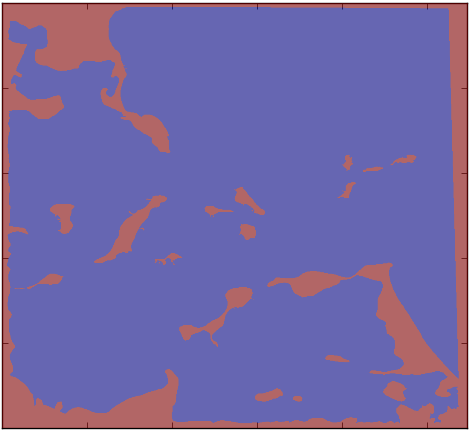
\includegraphics[width=\textwidth]{Fig_blankMap.png}
        \caption{{\small Environment with terrain: \\ Massachusetts Bay and surrounding area. }}    
        \label{fig:env_terrain}
    \end{subfigure}
    \hfill
    \begin{subfigure}[b]{0.475\textwidth}  
        \centering 
        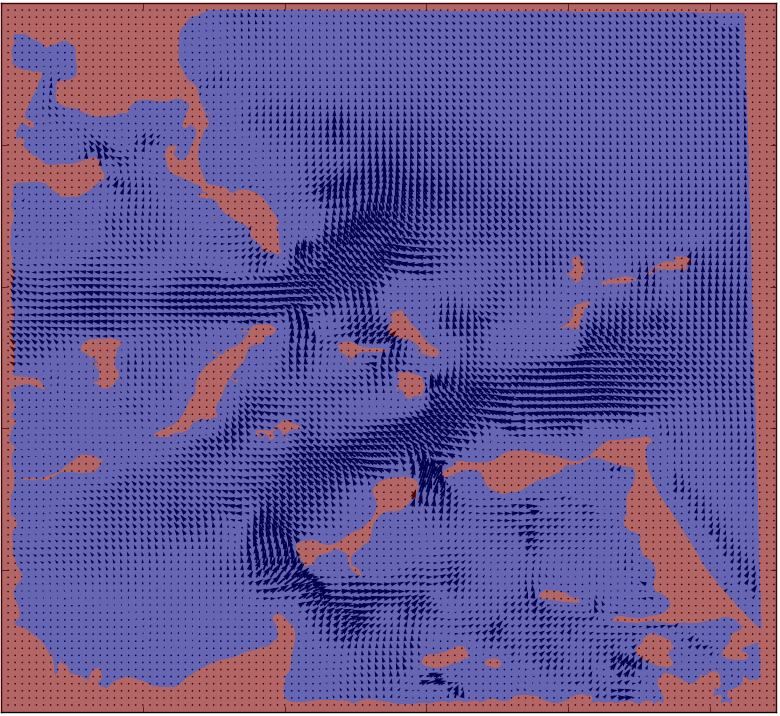
\includegraphics[width=\textwidth]{Fig_currentsMap.png}
        \caption{{\small Environment with water currents, \\ obtained from NECOFS forecast.}}   
        \label{fig:env_currents}
    \end{subfigure}
    \vskip\baselineskip
    \begin{subfigure}[b]{0.475\textwidth}   
        \centering 
        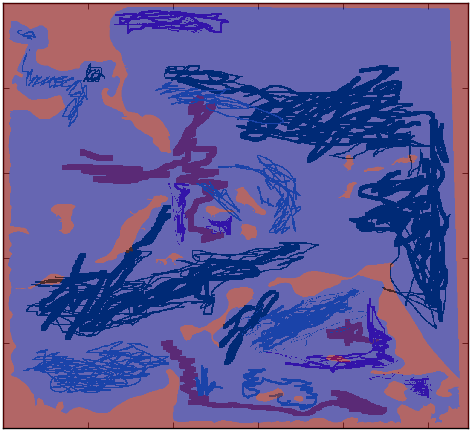
\includegraphics[width=\textwidth]{Fig_entitiesMap.png}
        \caption{{\small Environment with (simulated) \\ subsurface entities under study by USV.}}
        \label{fig:env_entities}
    \end{subfigure}
    \quad
    \begin{subfigure}[b]{0.475\textwidth}   
        \centering 
        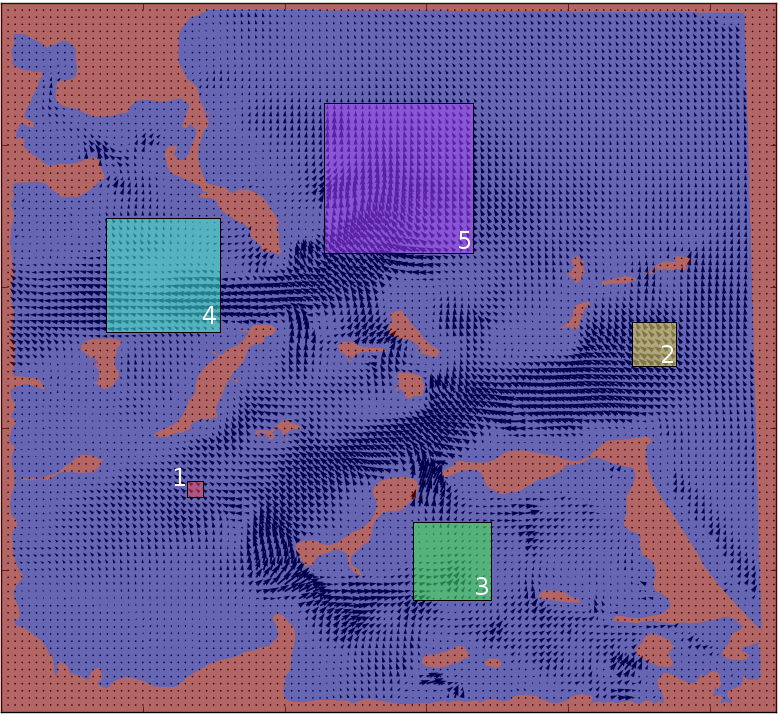
\includegraphics[width=\textwidth]{CurrentsTargetMap.png}
        \caption{{\small Environment with example target \\ regions $R_1, R_2, .., R_5$}}   
        \label{fig:env_targets}
    \end{subfigure}
    \caption[Environment overview.]{Environment overview.}
    \label{fig:env}
\end{figure}
%%%%%%%%%%%%%%%%%%%%%%%%%%
% End experimental Setup %
%%%%%%%%%%%%%%%%%%%%%%%%%%

%%%%%%%%%%%%%%%%%%%%%%%%%%%%%%%%%
% Water currents time intervals %
%%%%%%%%%%%%%%%%%%%%%%%%%%%%%%%%%
\begin{figure}[H]
    \captionsetup{justification=centering}
    \centering
    \begin{subfigure}[b]{0.475\textwidth}
        \centering
        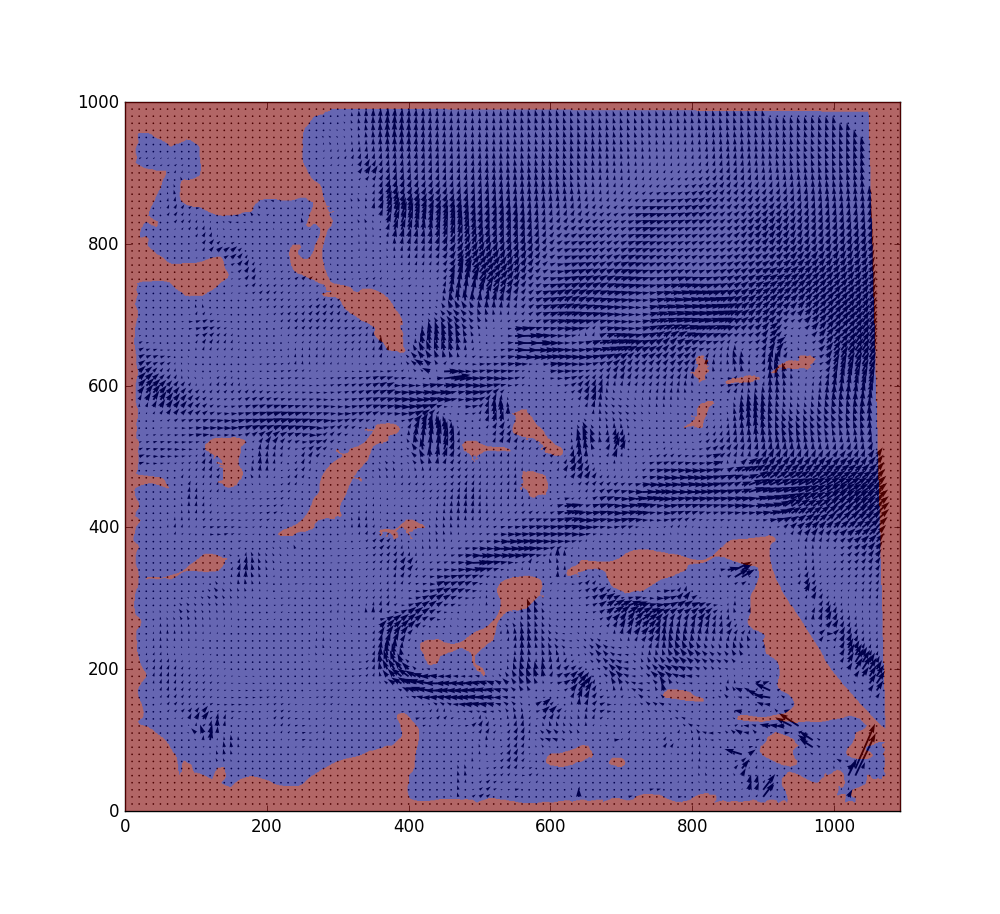
\includegraphics[width=\textwidth,trim={3cm 3cm 3cm 3cm},clip]{Fig_currentsMap-1.png}
        \caption{{\small Water currents at $t = 0 (min)$, $t_{interval} = 1$}}    
        \label{fig:currents_interval_1}
    \end{subfigure}
    \hfill
    \begin{subfigure}[b]{0.475\textwidth}  
        \centering 
        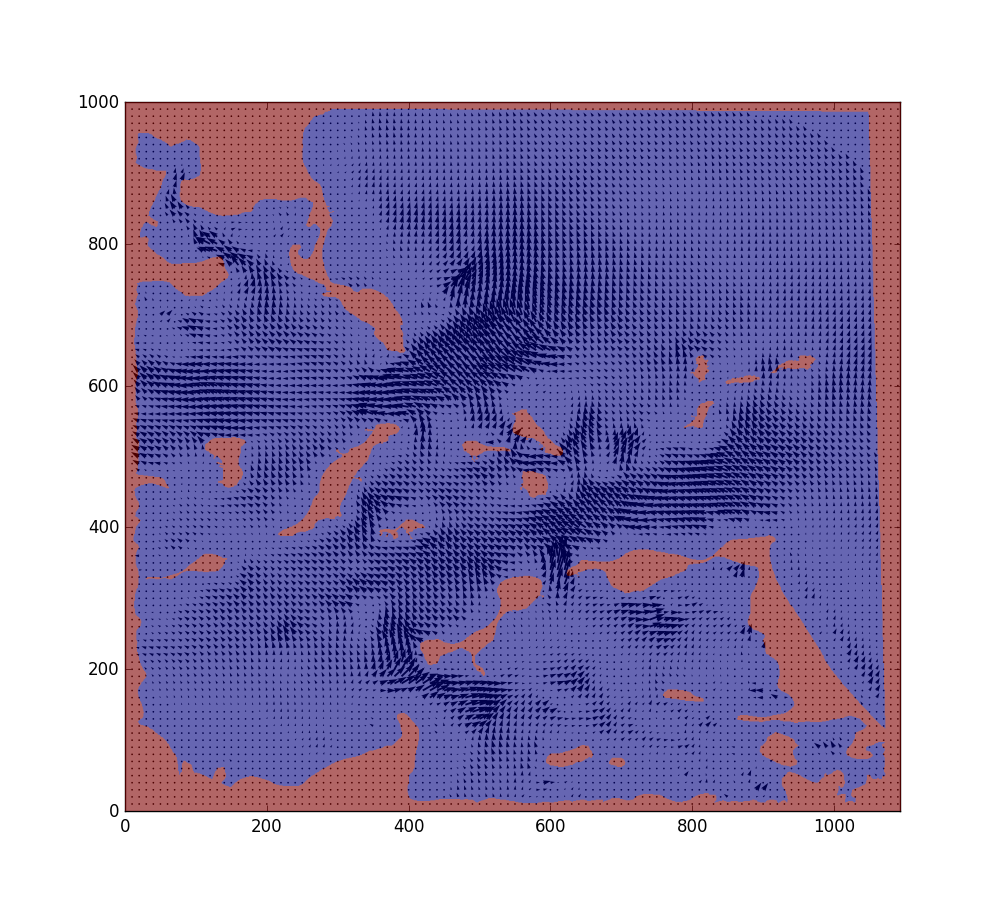
\includegraphics[width=\textwidth,trim={3cm 3cm 3cm 3cm},clip]{Fig_currentsMap-3.png}
        \caption{{\small Water currents at $t = 60 (min)$, $t_{interval} = 3$}}   
        \label{fig:currents_interval_3}
    \end{subfigure}
    \vskip\baselineskip
    \begin{subfigure}[b]{0.475\textwidth}   
        \centering 
        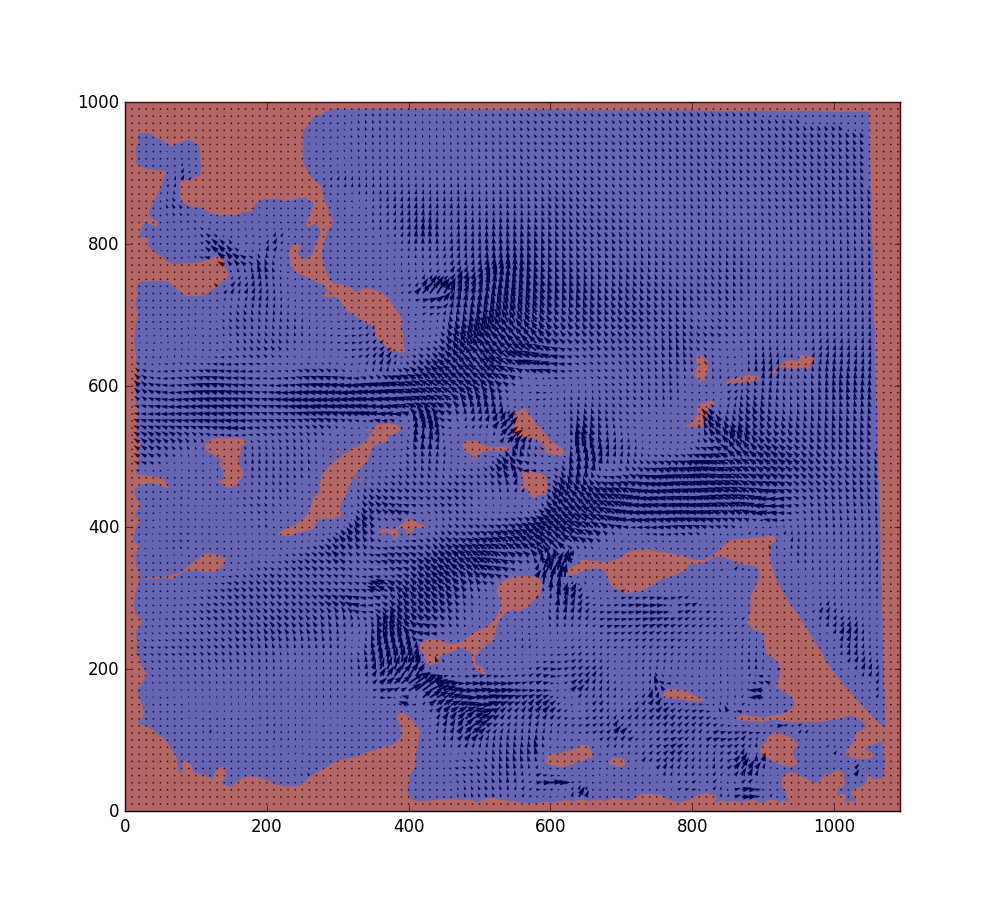
\includegraphics[width=\textwidth,trim={3cm 3cm 3cm 3cm},clip]{Fig_currentsMap-5.png}
        \caption{{\small Water currents at $t = 120 (min)$, $t_{interval} = 5$}}   
        \label{fig:currents_interval_5}
    \end{subfigure}
    \quad
    \begin{subfigure}[b]{0.475\textwidth}   
        \centering 
        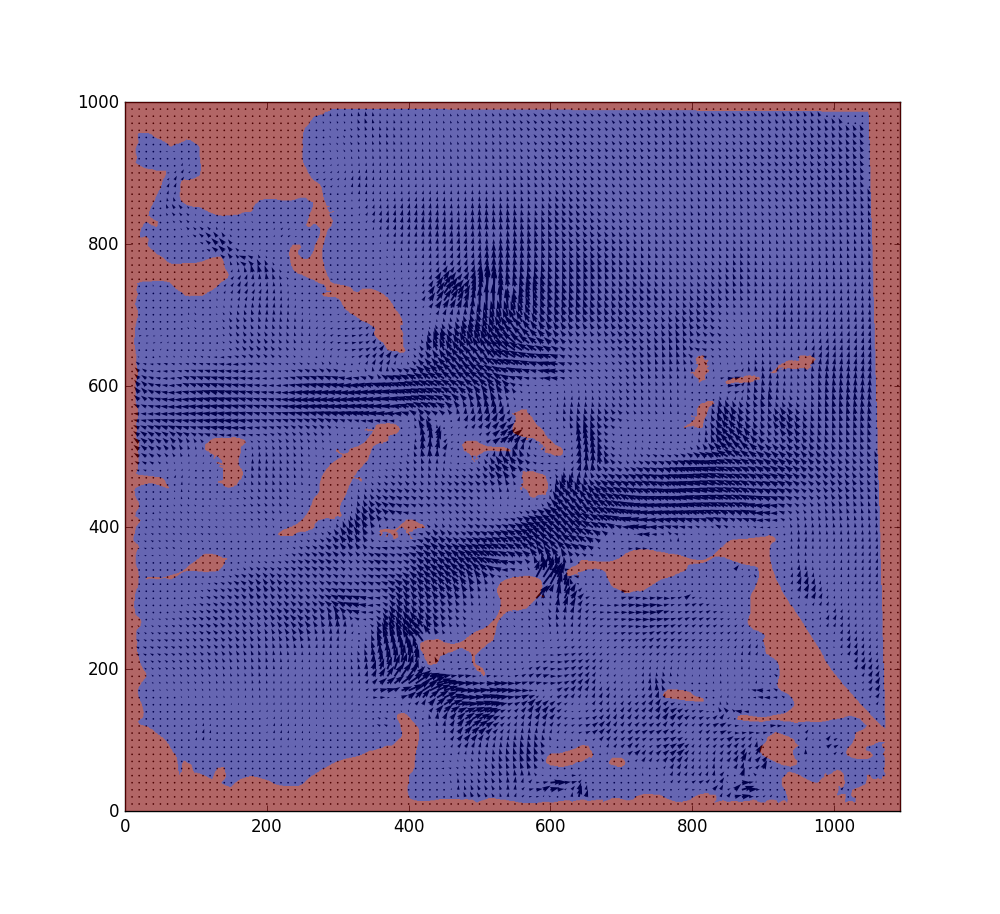
\includegraphics[width=\textwidth,trim={3cm 3cm 3cm 3cm},clip]{Fig_currentsMap-7.png}
        \caption[interval 7]%
        {{\small Water currents at $t = 180 (min)$, $t_{interval} = 7$}}   
        \label{fig:currents_interval_7}
    \end{subfigure}
    \caption[Dynamic water currents.]{Water currents vary over time $t$ and are stored in discrete intervals $t_{interval}$.} 
    \label{fig:currents_intervals}
\end{figure}
%%%%%%%%%%%%%%%%%%%%%%%%%%%%%%%%%%%%%
% End Water currents time intervals %
%%%%%%%%%%%%%%%%%%%%%%%%%%%%%%%%%%%%%

%%%%%%%%%%%%%%%%%
% System params %
%%%%%%%%%%%%%%%%%
\begin{table}[H]\small
    \begin{tabular}{|l|l|l|}
    \hline
    USV speed (cells per minute) & Water current update interval (minutes) & Water current forecast duration (hours) \\
    \hline
    154                 & 30                                      & 24 \\
    \hline
    \end{tabular}
    \caption{System settings}
    \label{sys_settings}
\end{table}


\begin{table}[H]\small
    \begin{tabular}{|l|l|l|l|l|l|l|l|l|l|}
\hline
ID & Score & Lon & Lat & Width & Length & Xpoints & Ypoints & Margin & Roam \\
\hline
1 & 100 & -70.970 & 42.300 & 10 & 10 & 10 & 10 & 1 & 0 \\
\hline
2 & 100 & -70.881 & 42.327 & 50 & 50 & 50 & 50 & 1 & 0 \\
\hline
3 & 100 & -70.920 & 42.287 & 100 & 100 & 100 & 100 & 1 & 0 \\
\hline
4 & 100 & -70.976 & 42.340 & 150 & 150 & 150 & 150 & 1 & 0 \\
\hline
5 & 100 & -70.930 & 42.348 & 200 & 200 & 200 & 200 & 1 & 0 \\
\hline  
        
    \end{tabular}
    \caption[Targets for mission planning.]{Targets for mission planning.}
    \label{tbl:targets}
\end{table}

\begin{table}[H]\small
    \begin{tabular}{|l|l|l|}
\hline
ID & Lon & Lat\\
\hline
1 & -70.9869 & 42.3035 \\
\hline  
    \end{tabular}
    \caption[Robot safepoints.]{Allowed safepoints where the robot must end mission at exactly one of these.}
    \label{tbl:safepoints}
\end{table}

\section{\textit{Surveyor} Results}

\subsection{\textit{Goto} Path Planning}

The \textit{Goto} planning results form the bulk of the analysis, and will be used to answer some of the questions posed in Section \ref{section:contributions}. A number of runs are analyzed with variation on the weights, but all are evaluated using six \textit{Goto} tasks. Three pairs of points are selected and each yields two tasks based on reversing the start and stop points. This reversal is to ensure that the water current impacts the system enough that the direction of planning affects the result over them same area. The six paths are described in Table \ref{tbl:goto_tasks}.

\begin{table}[H]\small
    \begin{tabular}{|l|l|l|l|l|l|l|l|l|l|l|l|}
    \hline
    \thead{Goto task} & \thead{Source \\ (node)}  & \thead{Source \\ (Lat)} & \thead{Source \\ (Lon)} 
                 &  \thead{Goal \\ (node)}  & \thead{Goal \\ (Lat)} & \thead{Goal \\ (Lon)}\\
    \hline
    1-A & 1 & 42.300 & -70.970 & 5 &  42.348 & -70.930 \\
    \hline
    1-B & 5 & 42.348 & -70.930 & 1 &  42.300 & -70.970 \\
    \hline
    2-A & 5 & 42.348 & -70.930 & 2 & -70.881 &  42.327 \\
    \hline
    2-B & 2 & -70.881 & 42.327 & 5 &  42.348 & -70.930 \\
    \hline
    3-A & 1 & 42.300 & -70.970 & 3 & -70.920 &  42.287 \\
    \hline
    3-B & 3 & -70.920 &  42.287 & 1 & 42.300 & -70.970  \\
    \hline
    \end{tabular}
    \caption[\textit{Goto} planner tasks.]{\textit{Goto} tasks for path planning experiments. Node labels correspond to the target IDs in \ref{fig:env_targets}, and the coordinates are the region's center.}
    \label{tbl:goto_tasks}
\end{table}

\subsubsection{Initial Visual Analysis}
\label{section:initial_results}

\textit{Goto} analysis begins with a visual check that the paths are reasonable and that the various optimization criteria affect paths in the way that would be expected. The initial weights were selected by trial and error during development of the fitness function. No attempt has been made to refine the weights to achieve a desired behavior other than checking that the obstacles are avoided and that the paths make reasonably efficient waypoint placement. The work and reward criteria are toggled off and on to see how they affect the path separately and together. The solution paths for this experiment are shown in Figures \ref{fig:Paths_1-A_1-B}, \ref{fig:Paths_1-A_1-B}, and \ref{fig:Paths_1-A_1-B}. Each figure contains subfigures where the left-hand subfigures are runs for the 'A' \textit{Goto} tasks and the right-hand are for 'B' between the same two points. In all cases, the obstacle avoidance and distance minimization criteria are enabled.

When work and reward are both disabled, the behavior is as expected. When a straight line exists between the points (Figures \ref{fig:Path_1-A_terrain_only}, \ref{fig:Path_1-B_terrain_only}), the waypoints align along that line. In the presence of obstacles, the waypoints are positioned to tightly approach the shoreline to avoid collision with minimal deviation. Since the work criteria is disabled, there is no difference in the problem when reversing the start and end points of a path. This is demonstrated by the low variability between 'A' and 'B' paths under terrain and distance-only optimization. When adding only work minimization, the paths exhibit some variation. In \textit{Task 1-A}, the currents support the mission and no visible change is made to the path. From the other direction, \textit{Task 1-B}, a path deviation is made to avoid currents that require additional energy consumption. Comparing \textit{Task 2-A} and \textit{Task 2-B}, the currents influence the decision of which direction to go when routing around an island obstacle. Subtle changes are similarly present in \textit{Task 3-A} and \textit{Task 3-B}. It should be acknowledged that some deviation is almost assured when using metaheuristic solvers, but it will be shown that the convergence is tight. That all scenarios showed stronger deviation with work considered than without suggests that the work optimization is behaving as expected. In all cases, the result when only reward is added shows huge deviation. These paths are clearly much longer than previously planned. When reward and work are incorporated, the reward maximization dominates the work minimization. Figures \ref{fig:Path_3-A_terrain_work_reward} and \ref{fig:Path_2-A_terrain_work_reward} do show some bounding of the path toward the solution without reward criteria. The first major observation of these experiments is that every path is affected by the additional criteria in ways that match expectation. Second, combined criteria exhibit characteristics of all criteria, but will require balancing to achieve the desired planning behavior.

%%%%%%%%%%%%%%%%%%%%%%%%%%%
% Goto paths for 1-A, 1-B %
%%%%%%%%%%%%%%%%%%%%%%%%%%%
\begin{figure}[H]
    \centering
    \begin{subfigure}[b]{0.4\textwidth}
        \centering
        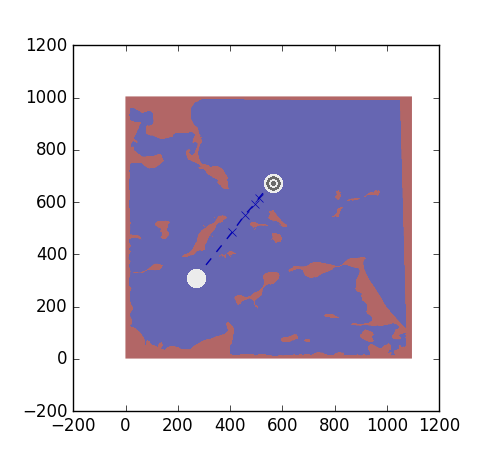
\includegraphics[width=\textwidth,trim={3cm 3cm 3cm 3cm},clip]{EXP3RG_PathAa_-1_-1_0_0.png}
        \caption{{\small Task 1-A, terrain only}}
        \label{fig:Path_1-A_terrain_only}
    \end{subfigure}
    \hfill
    \begin{subfigure}[b]{0.4\textwidth}  
        \centering 
        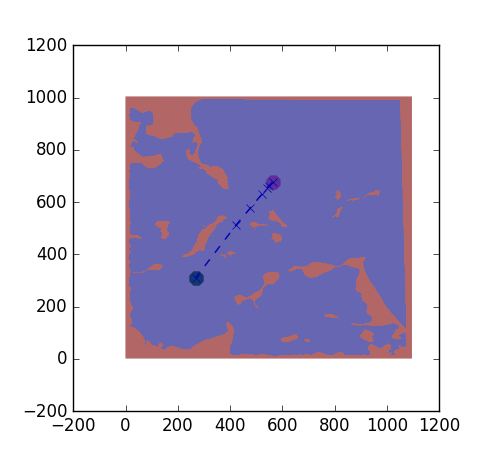
\includegraphics[width=\textwidth,trim={3cm 3cm 3cm 3cm},clip]{EXP3RG_PathAb_-1_-1_0_0.png}
        \caption{{\small Task 1-B, terrain only}}   
        \label{fig:Path_1-B_terrain_only}
    \end{subfigure}
    
    \begin{subfigure}[b]{0.4\textwidth}
        \centering
        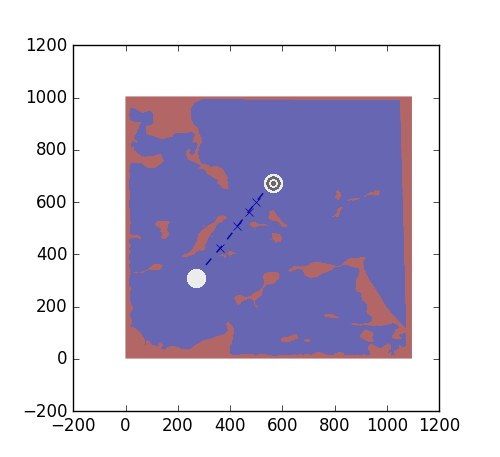
\includegraphics[width=\textwidth,trim={3cm 3cm 3cm 3cm},clip]{EXP3RG_PathAa_-1_-1_-1_0.png}
        \caption{{\small Task 1-A, terrain + work}}    
        \label{fig:Path_1-A_terrain_work}
    \end{subfigure}
    \hfill
    \begin{subfigure}[b]{0.4\textwidth}  
        \centering 
        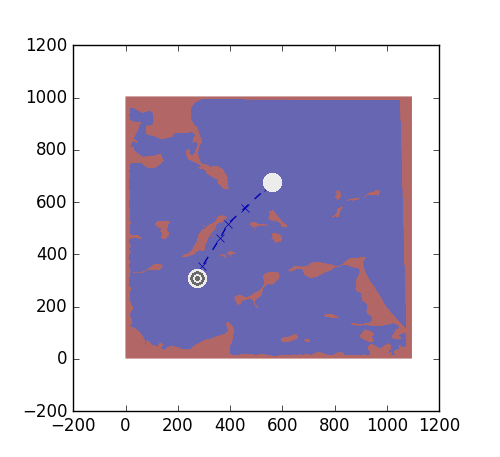
\includegraphics[width=\textwidth,trim={3cm 3cm 3cm 3cm},clip]{EXP3RG_PathAb_-1_-1_-1_0.png}
        \caption{{\small Task 1-B, terrain + work}}   
        \label{fig:Path_1-B_terrain_work}
    \end{subfigure}

    \begin{subfigure}[b]{0.4\textwidth}
        \centering
        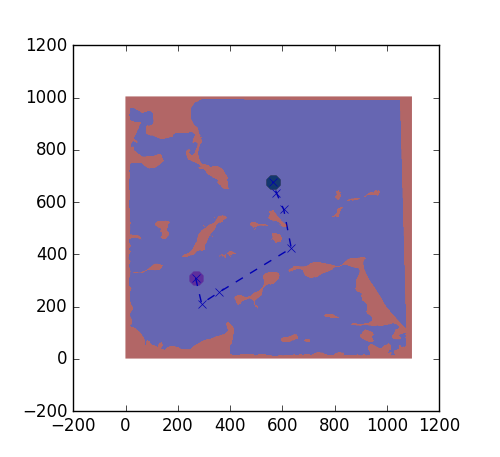
\includegraphics[width=\textwidth,trim={3cm 3cm 3cm 3cm},clip]{EXP3RG_PathAa_-1_-1_0_-1.png}
        \caption{{\small Task 1-A, terrain + reward}}    
        \label{fig:Path_1-A_terrain_reward}
    \end{subfigure}
    \hfill
    \begin{subfigure}[b]{0.4\textwidth}  
        \centering 
        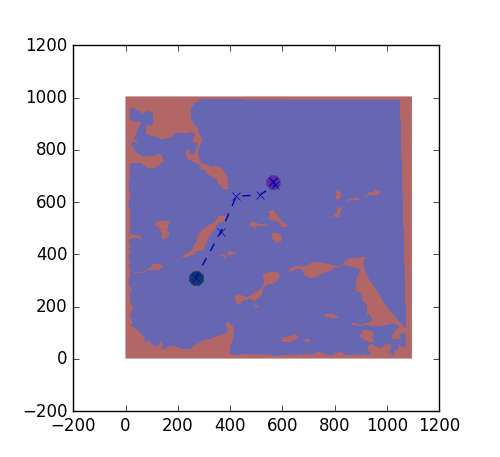
\includegraphics[width=\textwidth,trim={3cm 3cm 3cm 3cm},clip]{EXP3RG_PathAb_-1_-1_0_-1.png}
        \caption{{\small Task 1-B, terrain + reward}}   
        \label{fig:Path_1-B_terrain_reward}
    \end{subfigure}
   
  \begin{subfigure}[b]{0.4\textwidth}
        \centering
        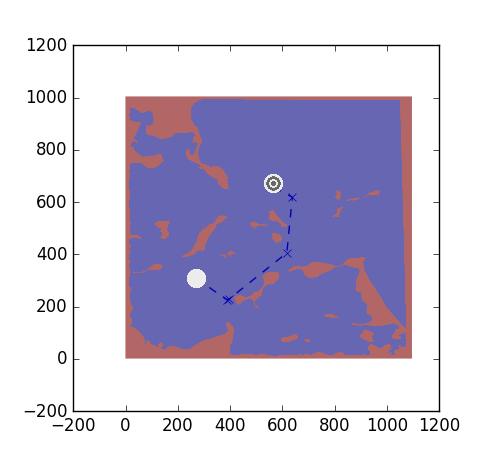
\includegraphics[width=\textwidth,trim={3cm 3cm 3cm 3cm},clip]{EXP3RG_PathAa_-1_-1_-1_-1.png}
        \caption{{\small Path 1-A, terrain + work + reward}}
        \label{fig:Path_1-A_terrain_work_reward}
    \end{subfigure}
    \hfill
    \begin{subfigure}[b]{0.4\textwidth}  
        \centering 
        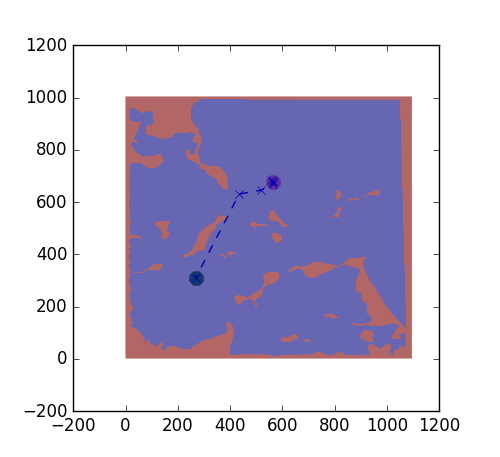
\includegraphics[width=\textwidth,trim={3cm 3cm 3cm 3cm},clip]{EXP3RG_PathAb_-1_-1_-1_-1.png}
        \caption{{\small Task 1-B, terrain + work + reward}}
        \label{fig:Path_5-B_terrain_work_reward}
    \end{subfigure}
      
    \caption{Solution paths for tasks 1-A and 1-B, with and without work and reward concerns.}
    \label{fig:Paths_1-A_1-B}
\end{figure}
%%%%%%%%%%%%%%%%%%%%%%%%%%%%%%
%End Goto paths for 1-A, 1-B %
%%%%%%%%%%%%%%%%%%%%%%%%%%%%%%

%%%%%%%%%%%%%%%%%%%%%%%%%%%
% Goto paths for 2-A, 2-B %
%%%%%%%%%%%%%%%%%%%%%%%%%%%
\begin{figure}[H]
    \centering
    \begin{subfigure}[b]{0.4\textwidth}
        \centering
        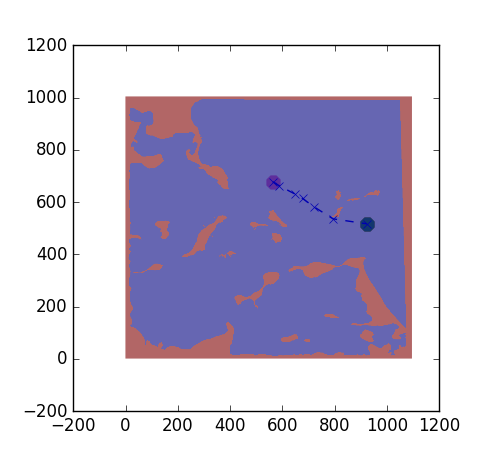
\includegraphics[width=\textwidth,trim={4cm 3cm 2cm 3cm},clip]{EXP3RG_PathBa_-1_-1_0_0.png}
        \caption{Task 2-A, terrain only}
        \label{fig:Path_2-A_terrain}
    \end{subfigure}
    \hfill
    \begin{subfigure}[b]{0.4\textwidth}  
        \centering 
        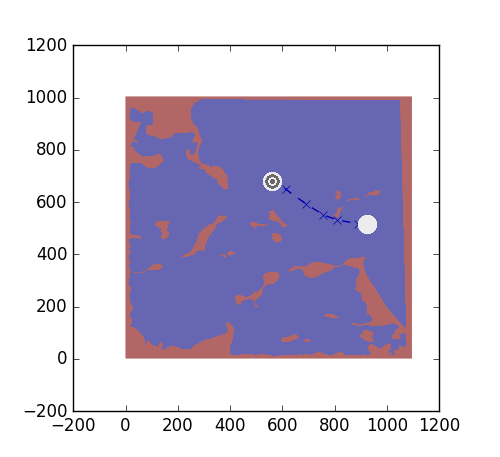
\includegraphics[width=\textwidth,trim={4cm 3cm 2cm 3cm},clip]{EXP3RG_PathBb_-1_-1_0_0.png}
        \caption{Task 2-B, terrain only}  
        \label{fig:Path_2-B_terrain}
    \end{subfigure}
    
    \begin{subfigure}[b]{0.4\textwidth}
        \centering
        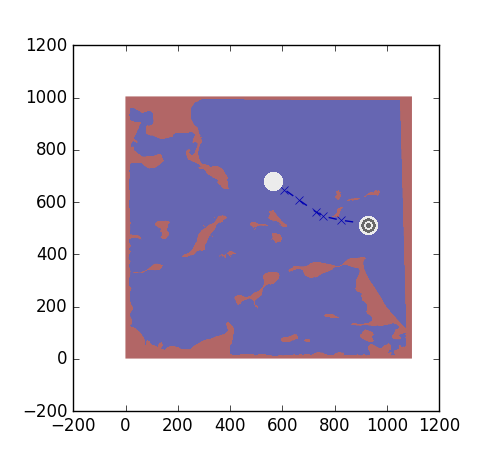
\includegraphics[width=\textwidth,trim={4cm 3cm 2cm 3cm},clip]{EXP3RG_PathBa_-1_-1_-1_0.png}
        \caption{Task 2-A, terrain + work}
        \label{fig:Path_2-A_terrain_work}
    \end{subfigure}
    \hfill
    \begin{subfigure}[b]{0.4\textwidth}  
        \centering 
        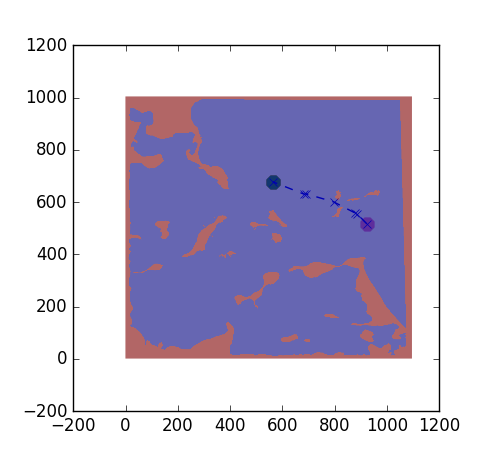
\includegraphics[width=\textwidth,trim={4cm 3cm 2cm 3cm},clip]{EXP3RG_PathBb_-1_-1_-1_0.png}
        \caption{Task 2-B, terrain + work}   
        \label{fig:Path_2-B_terrain_work}
    \end{subfigure}

    \begin{subfigure}[b]{0.4\textwidth}
        \centering
        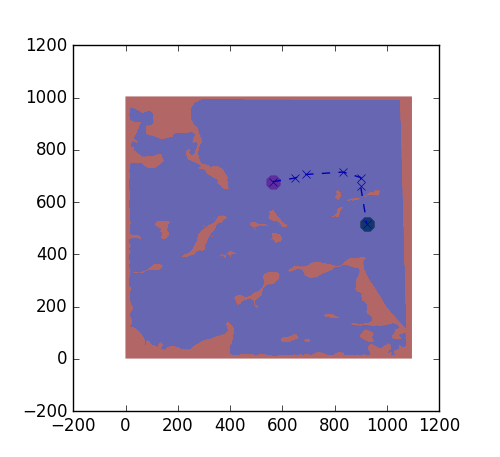
\includegraphics[width=\textwidth,trim={4cm 3cm 2cm 3cm},clip]{EXP3RG_PathBa_-1_-1_0_-1.png}
        \caption{Task 2-A, terrain + reward}
        \label{fig:Path_2-A_terrain_reward}
    \end{subfigure}
    \hfill
    \begin{subfigure}[b]{0.4\textwidth}  
        \centering 
        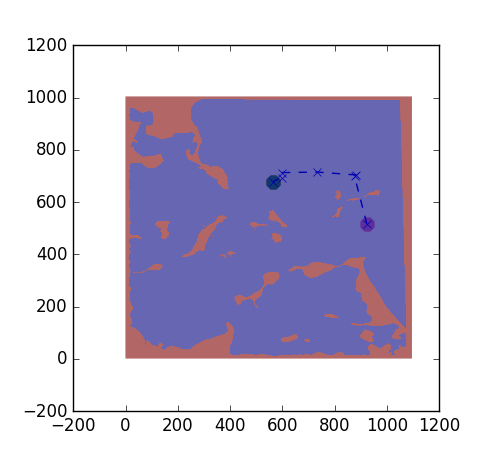
\includegraphics[width=\textwidth,trim={4cm 3cm 2cm 3cm},clip]{EXP3RG_PathBb_-1_-1_0_-1.png}
        \caption{Task 2-B, terrain + reward}
        \label{fig:Path_2-B_terrain_reward}
    \end{subfigure}
    
  \begin{subfigure}[b]{0.4\textwidth}
        \centering
        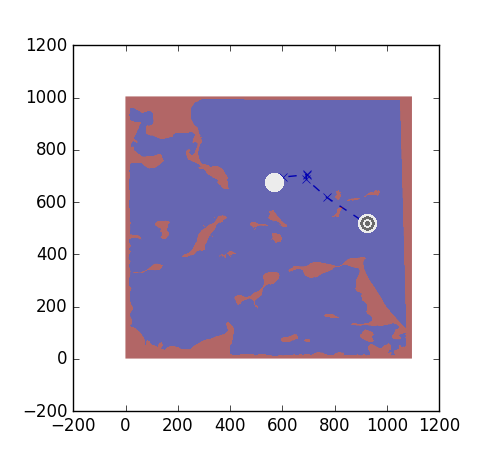
\includegraphics[width=\textwidth,trim={4cm 3cm 2cm 3cm},clip]{EXP3RG_PathBa_-1_-1_-1_-1.png}
        \caption{{\small Task 2-A, terrain + work + reward}}    
        \label{fig:Path_2-A_terrain_work_reward}
    \end{subfigure}
    \hfill
    \begin{subfigure}[b]{0.4\textwidth}  
        \centering 
        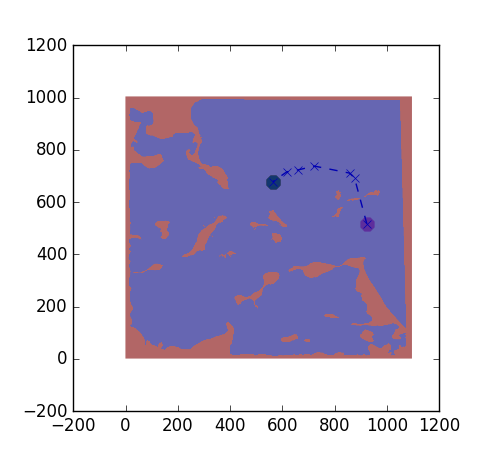
\includegraphics[width=\textwidth,trim={4cm 3cm 2cm 3cm},clip]{EXP3RG_PathBb_-1_-1_-1_-1.png}
        \caption{Task 2-B, terrain + work + reward} 
        \label{fig:Path_2-B_terrain_work_reward}
    \end{subfigure}

    \caption{Solution paths for tasks 2-A and 2-B, with and without work and reward concerns.}
    \label{fig:Paths_2-A_2-B}
\end{figure}
%%%%%%%%%%%%%%%%%%%%%%%%%%%%%%
%End Goto paths for 2-A, 2-B %
%%%%%%%%%%%%%%%%%%%%%%%%%%%%%%

%%%%%%%%%%%%%%%%%%%%%%%%%%%
% Goto paths for 3-A, 3-B %
%%%%%%%%%%%%%%%%%%%%%%%%%%%
\begin{figure}[H]
    \centering
    \begin{subfigure}[b]{0.4\textwidth}
        \centering
        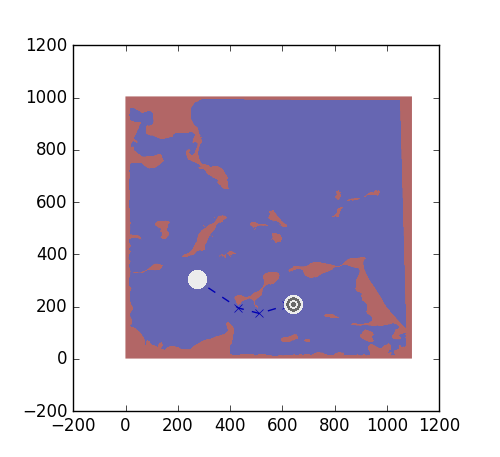
\includegraphics[width=\textwidth,trim={4cm 3cm 2cm 3cm},clip]{EXP3RG_PathCa_-1_-1_0_0.png}
        \caption{Task 3-A, terrain only}
        \label{fig:Path_3-A_terrain}
    \end{subfigure}
    \hfill
    \begin{subfigure}[b]{0.4\textwidth}  
        \centering 
        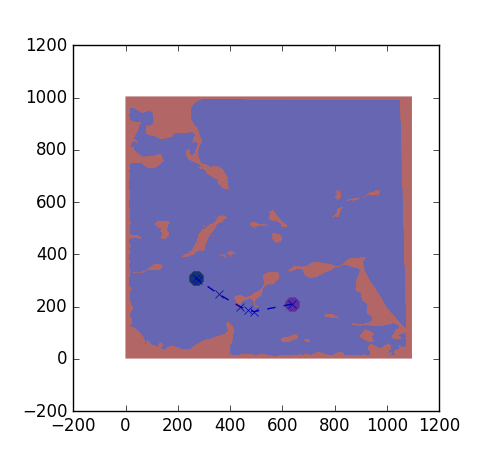
\includegraphics[width=\textwidth,trim={4cm 3cm 2cm 3cm},clip]{EXP3RG_PathCb_-1_-1_0_0.png}
        \caption{Task 3-B, terrain only}
        \label{fig:Path_3-B_terrain}
    \end{subfigure}
    \vskip\baselineskip   
    
    \begin{subfigure}[b]{0.4\textwidth}
        \centering
        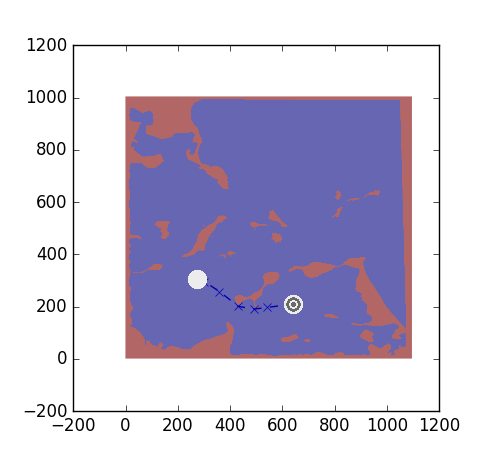
\includegraphics[width=\textwidth,trim={4cm 3cm 2cm 3cm},clip]{EXP3RG_PathCa_-1_-1_-1_0.png}
        \caption{ Task 3-A, terrain + work}
        \label{fig:Path_3-A_terrain_work}
    \end{subfigure}
    \hfill
    \begin{subfigure}[b]{0.4\textwidth}  
        \centering 
        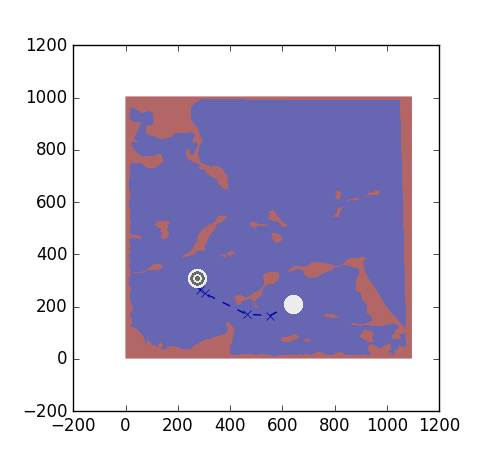
\includegraphics[width=\textwidth,trim={4cm 3cm 2cm 3cm},clip]{EXP3RG_PathCb_-1_-1_-1_0.png}
        \caption{\small Task 3-B, terrain + work}
        \label{fig:Path_3-B_terrain_work}
    \end{subfigure}

    \begin{subfigure}[b]{0.4\textwidth}
        \centering
        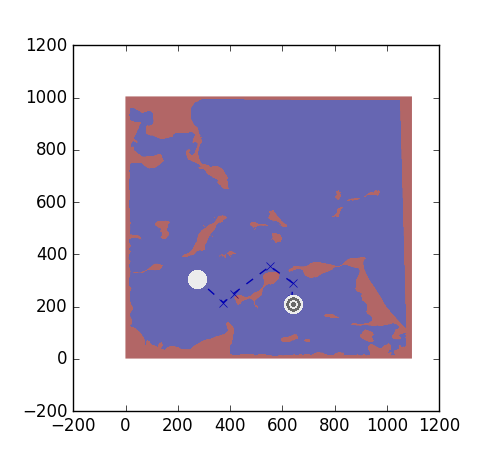
\includegraphics[width=\textwidth,trim={4cm 3cm 2cm 3cm},clip]{EXP3RG_PathCa_-1_-1_0_-1.png}
        \caption{Task 3-A, terrain + reward}  
        \label{fig:Path_3-A_terrain_reward}
    \end{subfigure}
    \hfill
    \begin{subfigure}[b]{0.4\textwidth}  
        \centering 
        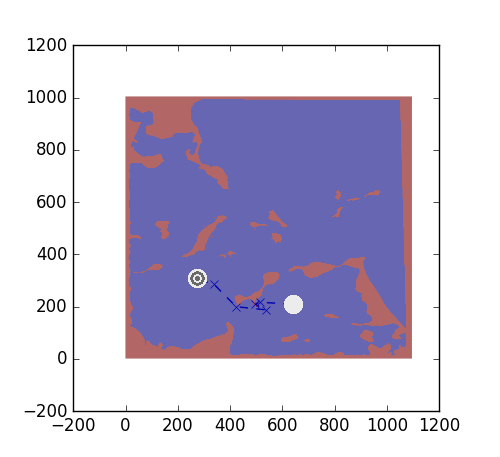
\includegraphics[width=\textwidth,trim={4cm 3cm 2cm 3cm},clip]{EXP3RG_PathCb_-1_-1_0_-1.png}
        \caption{Task 3-B, terrain + reward}
        \label{fig:Path_3-B_terrain_reward}
    \end{subfigure}
    
  \begin{subfigure}[b]{0.4\textwidth}
        \centering
        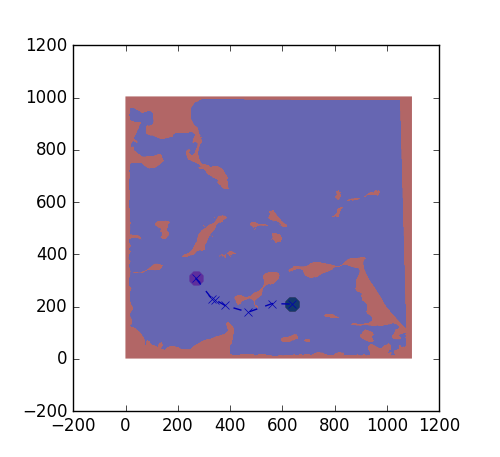
\includegraphics[width=\textwidth,trim={4cm 3cm 2cm 3cm},clip]{EXP3RG_PathCa_-1_-1_-1_-1.png}
        \caption{Task 3-A, terrain + work + reward}
        \label{fig:Path_3-A_terrain_work_reward}
    \end{subfigure}
    \hfill
    \begin{subfigure}[b]{0.4\textwidth}  
        \centering 
        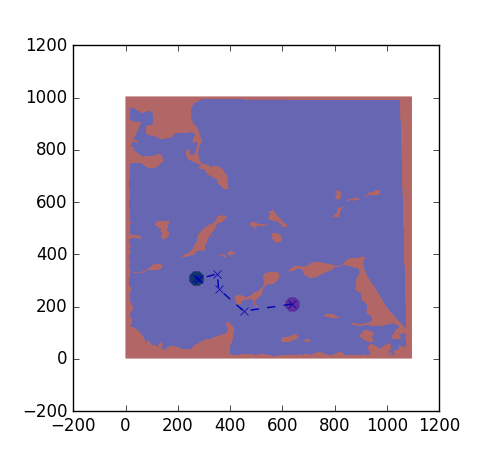
\includegraphics[width=\textwidth,trim={4cm 3cm 2cm 3cm},clip]{EXP3RG_PathCb_-1_-1_-1_-1.png}
        \caption{Task 3-B, terrain + work + reward}
        \label{fig:Path_3-B_terrain_work_reward}
    \end{subfigure}

    \caption{Solution paths for tasks 3-A and 3-B, with and without work and reward concerns.} 
    \label{fig:Paths_3-A_3-B}
\end{figure}
%%%%%%%%%%%%%%%%%%%%%%%%%%%%%%
%End Goto paths for 3-A, 3-B %
%%%%%%%%%%%%%%%%%%%%%%%%%%%%%%

\subsubsection{Comparison of Metaheuristic Planning Algorithms}

The four metaheuristic algorithms discussed in Section \label{section:goto} are applied to path planning used the fitness function in Section \ref{section:fitness_function}. The initial results in Section \ref{section:initial_results} used PSO, which was arbitrarily chosen. A suitable algorithm repeatedly reaches an approximately optimal solution within a bounded number of iterations. While some deviation is tolerated due to the stochastic nature of the algorithms, there should be a tight bound on the solutions reached. The algorithms will be compared on their convergence speed and width, and the quality and bound on the path characteristics. The comparisons are made with and without optimizing reward and work in order to see how more complicated set of criteria compare to the more common distance minimization. The convergence curves for 10 runs without work and reward optimization are shown in Figures \ref{fig:convergence_a_PSO}, \ref{fig:convergence_a_BEE}, \ref{fig:convergence_a_DE}, and \ref{fig:convergence_a_SGA} for PSO, BEE, DE and GA, respectively. Their convergence when work and reward is added is shown in Figures \ref{fig:convergence_b_PSO}, \ref{fig:convergence_b_BEE}, \ref{fig:convergence_b_DE}, and \ref{fig:convergence_b_SGA}. In each, the dashed horizontal line indicates the fitness of the the best solution in the ten runs (minimized). For easier comparison, the average convergence is shown for all four in Figure \ref{fig:convergence_a_avg} (terrain only) and in Figure \ref{fig:convergence_b_avg}.Box plots of each path characteristic (distance, duration, work, and reward) for these runs when not optimizing work and reward are shown in Figures \ref{fig:algcompare_a_distance}, \ref{fig:algcompare_a_duration}, \ref{fig:algcompare_a_work}, and \ref{fig:algcompare_a_reward}. The same comparisons are made for the runs using work and reward in Figures \ref{fig:algcompare_b_distance}, \ref{fig:algcompare_b_duration}, \ref{fig:algcompare_b_work}, and \ref{fig:algcompare_b_reward}. Iterations are a valid comparison for these algorithms; their runtimes are dominated by the time spent evaluating the complex fitness function so each iteration is approximately the same speed across all four. 

First consider the results where the work and reward were not optimized. The older, evolutionary algorithms, GA and DE, have best fitness values of 520.15 and 515.57, respectively. The more recent, colony-behavior algorithms, BEE and PSO perform much better with values of 405.10 and 398.06. With only ten runs, the differences are to slight to choose a clear winner between PSO and BEE, but are over 100 below the other two. In the best case, PSO and BEE are better. The width of the runs echo the results of the best fitness comparison. The spread of GA is still very wide and indicates that the solutions have not converged after 100 iterations. The other three show some degree of convergence, with a moderate width of 223.67 for DE and the very tight widths 73.88 and 22.44 for BEE and PSO, respectively. Again, PSO wins. Similarly, the speed of convergence outcomes show order the algorithms, from worst to best: GA, DE, BEE, and PSO. While PSO is not hugely different than BEE, it does perform the best in terms of best fitness, fitness distribution, and convergence speed.

The fitness function combines the criteria in such a way that it captures the impact of all four criteria in a way that the path planning behaves in a desired way. It is possible for a fitness function to fail to capture the relative worth of a path. Thus, the path measurements of distance, duration, work, and reward need to be checked to verify that a path with higher fitness actually is better. Figure \ref{fig:algcompare_a_distance} shows that PSO better minimizes the distance, both in the best case and in having a narrower spread. PSO's box plot is very tight (width of 1274.51), especially compared to the high spread of GA and DE, whose widths are 7183.74 and 2514.64. This pattern continues when looking at the distribution of duration (\ref{fig:algcompare_a_duration}), work (\ref{fig:algcompare_a_work}), and reward (\ref{fig:algcompare_a_reward}). These distributions strongly suggest that the lower fitness values correspond to higher-quality path planning, and that PSO is the best algorithm for its optimization and reliability. 

Next, the situation is made more complicated with the addition of work minimization and reward maximization. Work's Joules and reward's nonunit values tend to run large, so the fitness in this situation should not be compared to fitness in the terrain-only situation. Using all three algorithms, the increased path planning complexity is reflected in the wider fitness spread and slowed convergence. GA shows especially poor performance, coming nowhere near convergence in the 100 iterations allowed. DE, BEE, and PSO show increasingly better performance. The best, PSO, is much less affected by the additional criteria than the others. The reliability of PSO compared to the others is further highlighted in the box plots showing spread of each path characteristic. As before, PSO maintains the tightest bounds on all criteria. GA continues to perform the worst. Every test has displayed a consistent ranking of algorithm quality, with one exception: DE's reward spread is worse than BEE, but does have a tighter spread making it more reliable. 

PSO has beaten the other three algorithms in all respects evaluated. It converges faster and with greater stability while also providing the best optimization for distance, duration, work and reward. Even though PSO is challenged by the greater complexity of multi-objective optimization (some of which are in opposition: work vs reward), it converges reasonably well in the 100 iterations allowed. All four algorithms are options in the system, but PSO is made to be the \textit{Surveyor}'s default \textit{Goto} path planning solver. 

%%%%%%%%%%%%%%%%%%%%%%%%%%%%%
% Goto planner PSO Settings %
%%%%%%%%%%%%%%%%%%%%%%%%%%%%%
\begin{table}[H]
    \begin{tabular}{|l|l|l|}
        \hline
        \thead{Generations} & \thead{Individuals \\ (Pool size)}  & \thead{Number of waypoints}  \\
        \hline
        100 & 100 & 5   \\
        \hline
    \end{tabular}
    \caption[Metaheurisic path planning solver settings.]{Settings common to all metaheuristic algorithms used. To avoid overfitting to the experimental setup, the algorithm-specific settings are unchanged from the PyGMO library defaults.}
    \label{tbl:meta_params}
\end{table}


%%%%%%%%%%%%%%%%%%%%%%%%%%%%%%%%%
% Convergence curves %
%%%%%%%%%%%%%%%%%%%%%%%%%%%%%%%%%
\begin{figure}[H]
    \captionsetup{justification=centering}
    \centering
        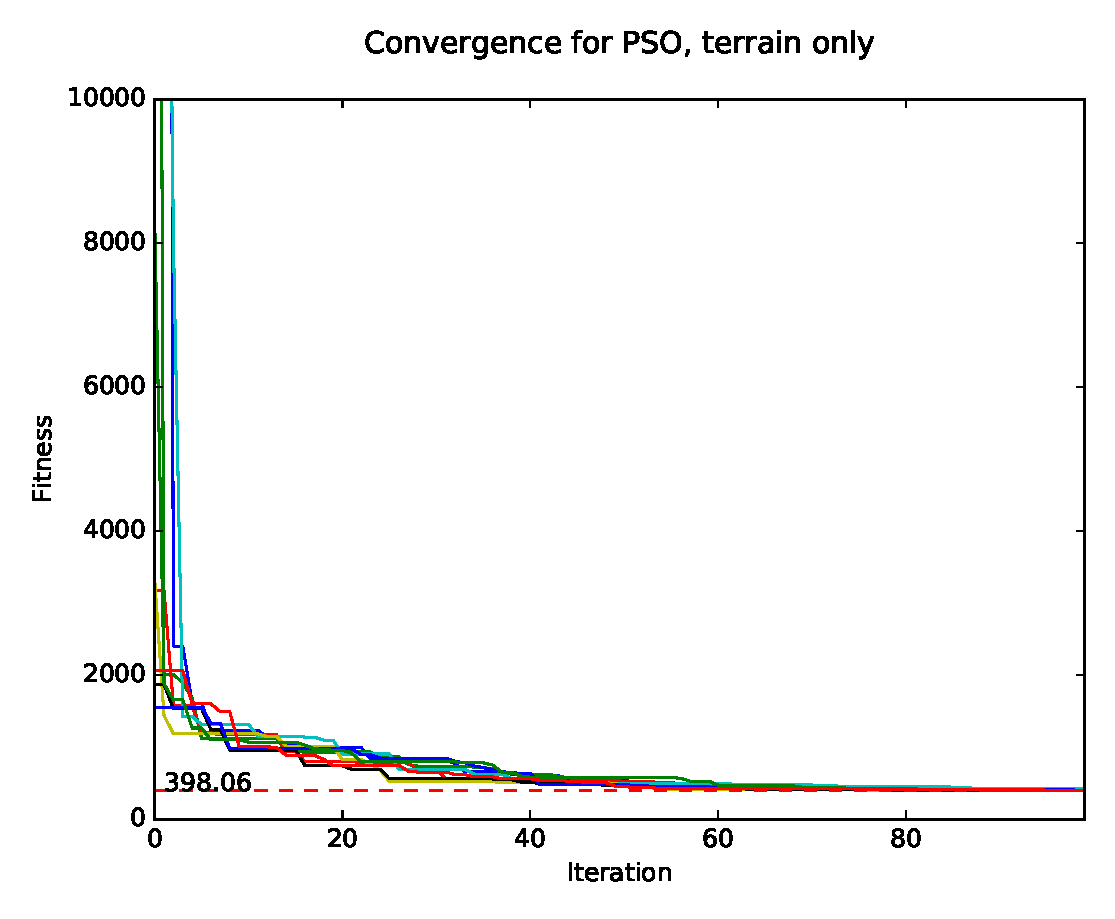
\includegraphics[width=0.75\textwidth,trim={0cm 0.75cm 0cm 0.75cm},clip]{conv_PSO_a.eps}
    \caption{Convergence for particle swarm optimization, not optimizing work and reward}
    \label{fig:convergence_a_PSO}
\end{figure}

\begin{figure}[H]
    \captionsetup{justification=centering}
    \centering
        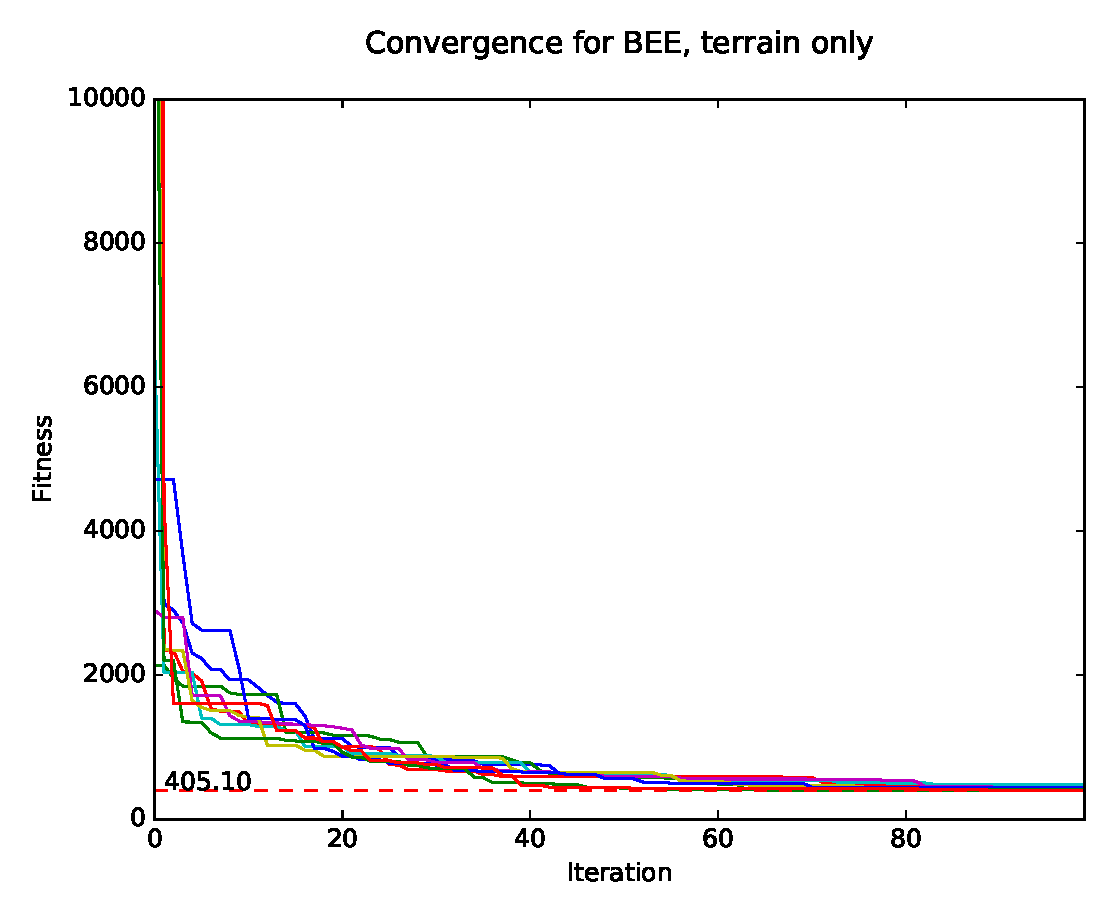
\includegraphics[width=0.75\textwidth,trim={0cm 0.75cm 0cm 0.75cm},clip]{conv_BEE_a.eps}
    \caption[]{Convergence for bee colony optimization, not optimizing work and reward}
    \label{fig:convergence_a_BEE}
\end{figure}

\begin{figure}[H]
    \captionsetup{justification=centering}
    \centering
        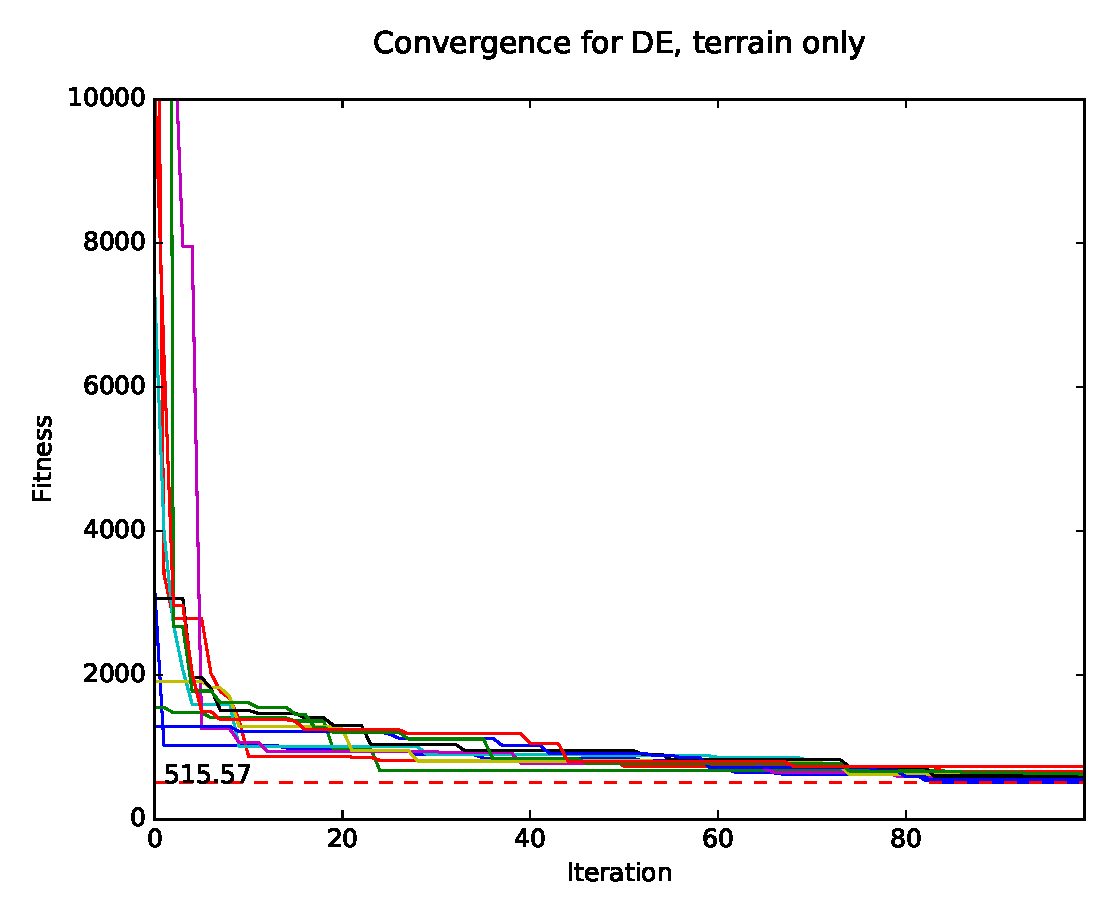
\includegraphics[width=0.75\textwidth,trim={0cm 0.75cm 0cm 0.75cm},clip]{conv_DE_a.eps}
    \caption{Convergence for differential evolution, not optimizing work and reward}
    \label{fig:convergence_a_DE}
\end{figure}

\begin{figure}[H]
    \captionsetup{justification=centering}
    \centering
        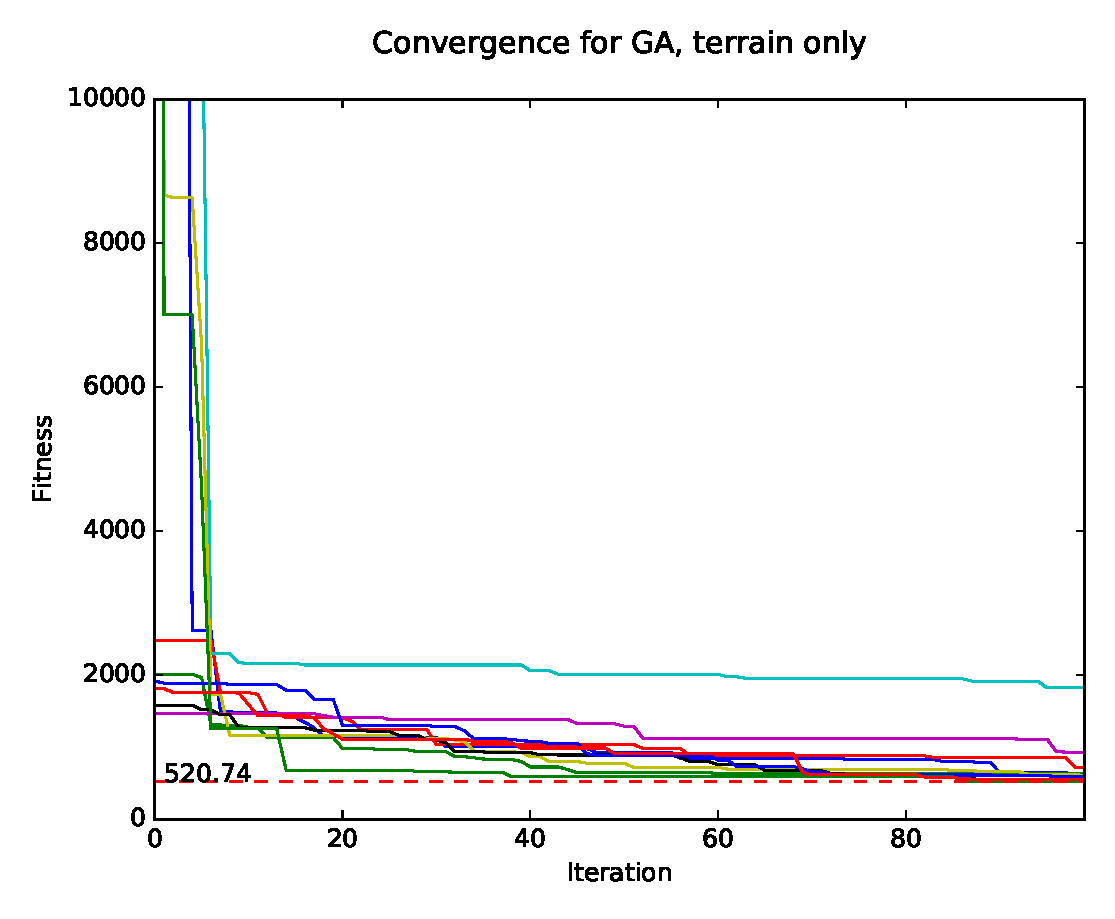
\includegraphics[width=0.75\textwidth,trim={0cm 0.75cm 0cm 0.75cm},clip]{conv_GA_a.eps}
    \caption{Convergence for genetic algorithm, not optimizing work and reward}
    \label{fig:convergence_a_SGA}
\end{figure}

\begin{figure}[H]
    \captionsetup{justification=centering}
    \centering
        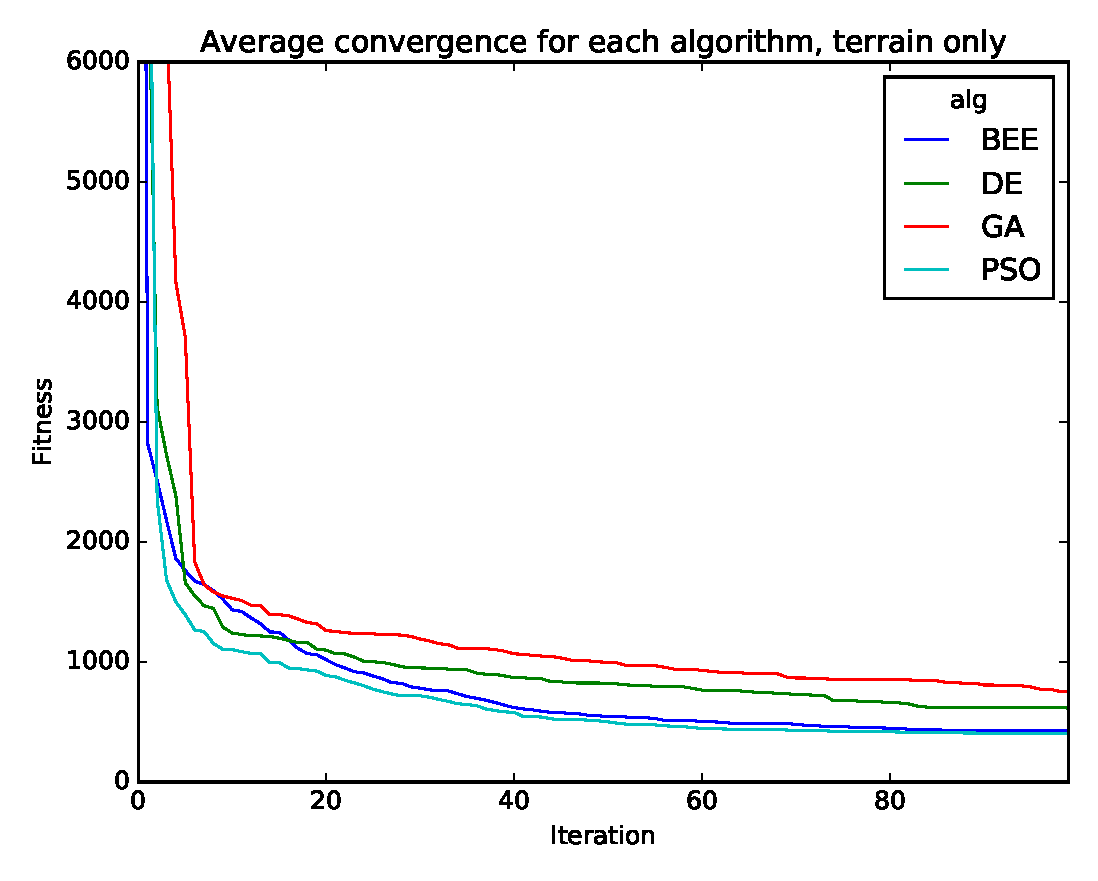
\includegraphics[width=0.75\textwidth,trim={0cm 0.75cm 0cm 0.75cm},clip]{conv_avg_a.eps}
    \caption{Average convergence for all algorithms, not optimizing work and reward}
    \label{fig:convergence_a_avg}
\end{figure}


\begin{figure}[H]
    \captionsetup{justification=centering}
    \centering
        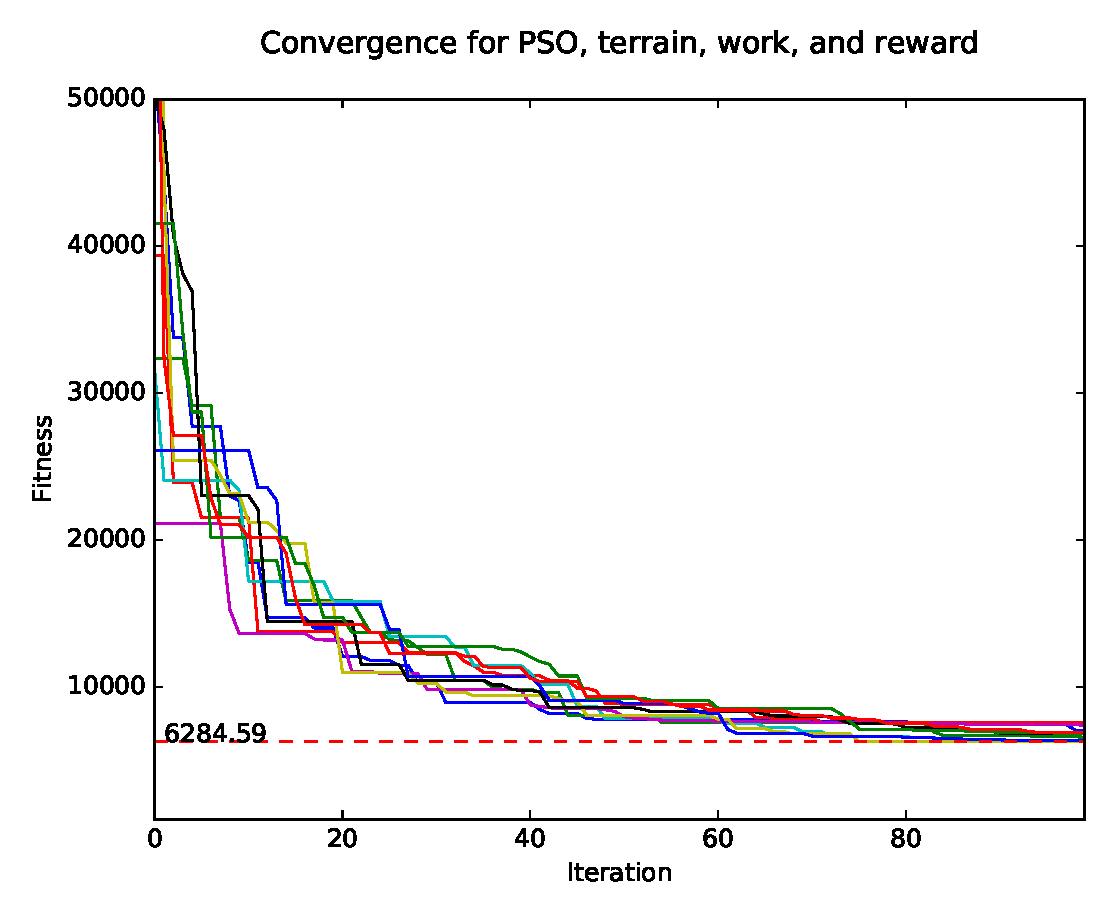
\includegraphics[width=0.75\textwidth,trim={0cm 0.75cm 0cm 0.75cm},clip]{conv_PSO_b.eps}
    \caption{Convergence for particle swarm optimization, optimizing work and reward}
    \label{fig:convergence_b_PSO}
\end{figure}

\begin{figure}[H]
    \captionsetup{justification=centering}
    \centering
        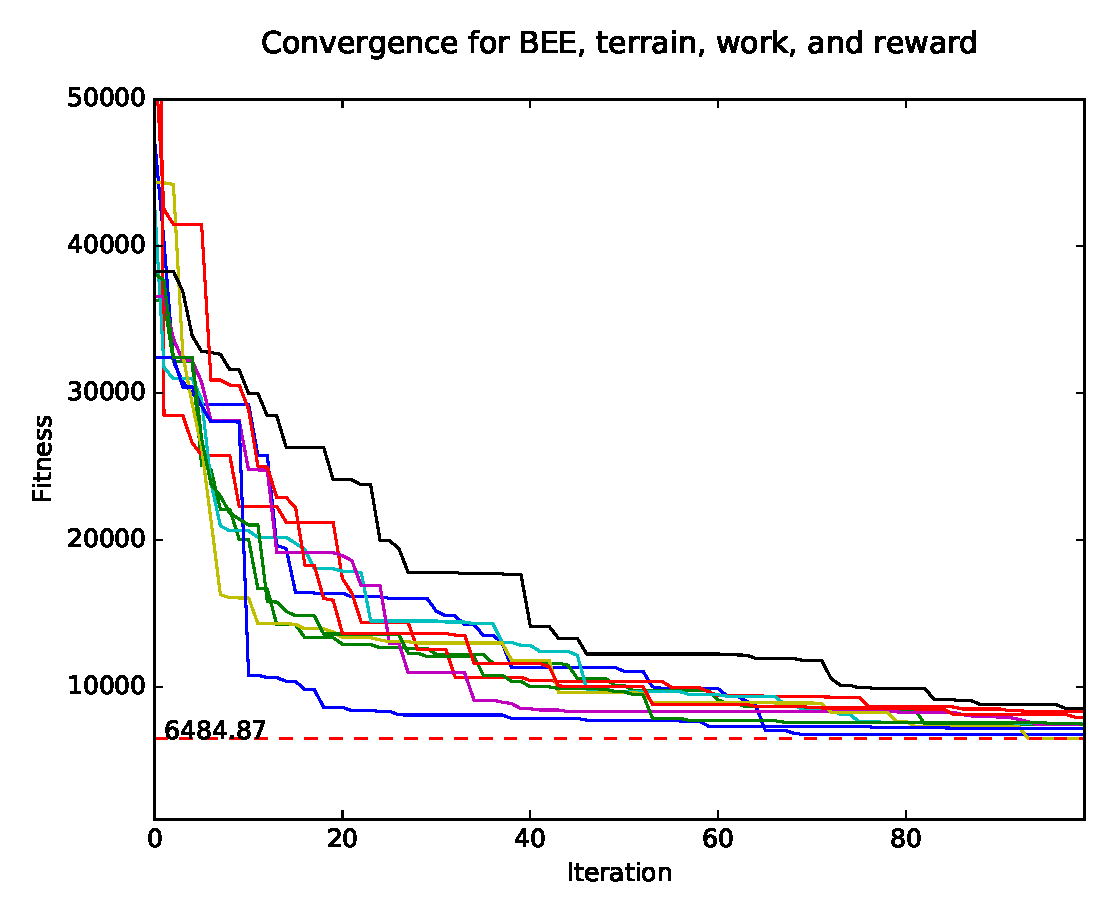
\includegraphics[width=0.75\textwidth,trim={0cm 0.75cm 0cm 0.75cm},clip]{conv_BEE_b.eps}
    \caption{Convergence for bee colony optimization, optimizing work and reward}
    \label{fig:convergence_b_BEE}
\end{figure}

\begin{figure}[H]
    \captionsetup{justification=centering}
    \centering
        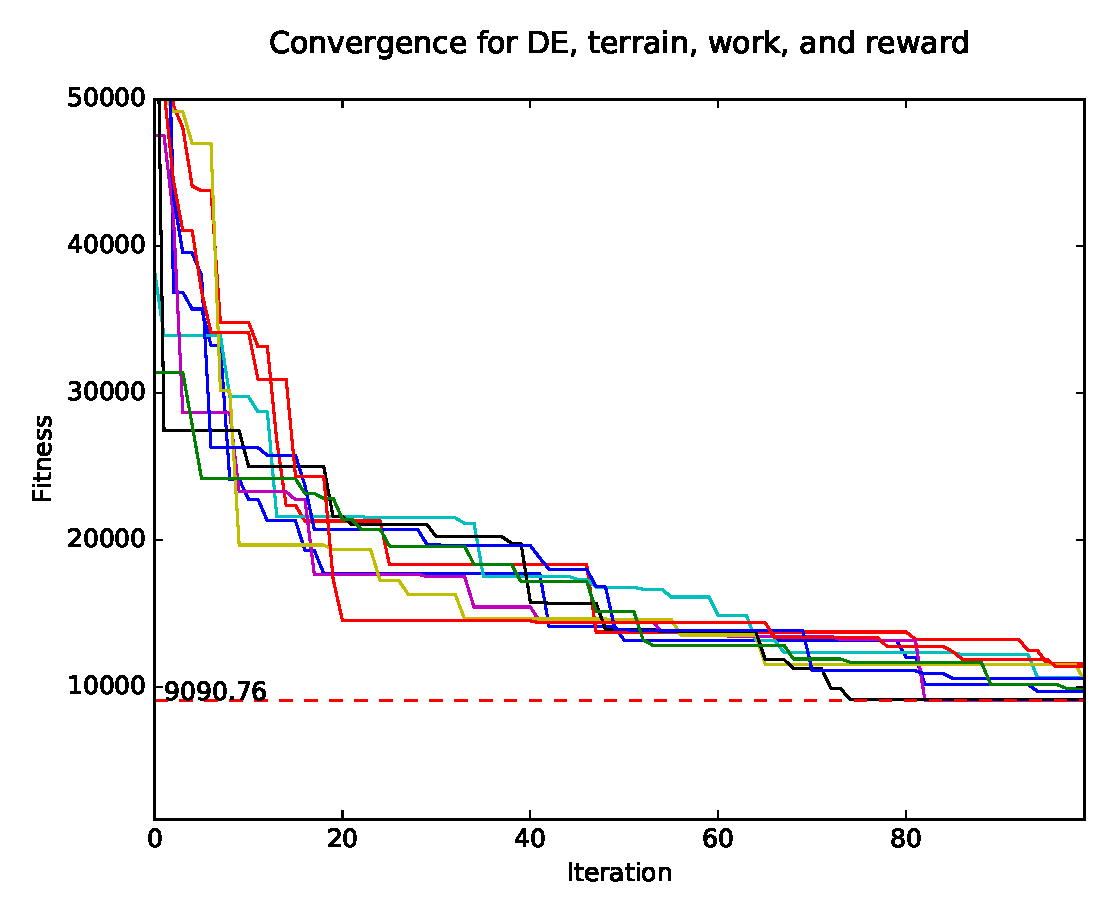
\includegraphics[width=0.75\textwidth,trim={0cm 0.75cm 0cm 0.75cm},clip]{conv_DE_b.eps}
    \caption{Convergence for differential evolution, optimizing work and reward}
    \label{fig:convergence_b_DE}
\end{figure}

\begin{figure}[H]
    \captionsetup{justification=centering}
    \centering
        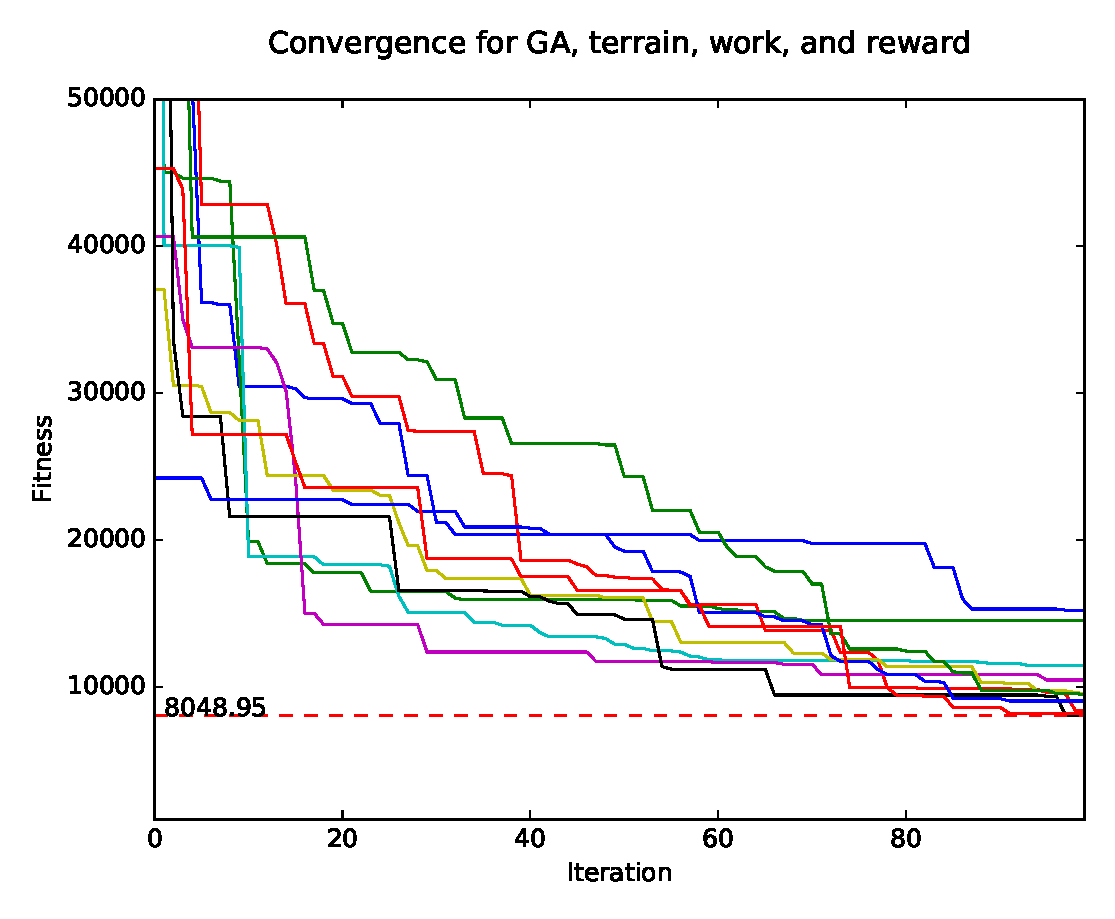
\includegraphics[width=0.75\textwidth,trim={0cm 0.75cm 0cm 0.75cm},clip]{conv_GA_b.eps}
    \caption{Convergence for genetic algorithm, optimizing work and reward}   
    \label{fig:convergence_b_SGA}
\end{figure}

\begin{figure}[H]
    \captionsetup{justification=centering}
    \centering
        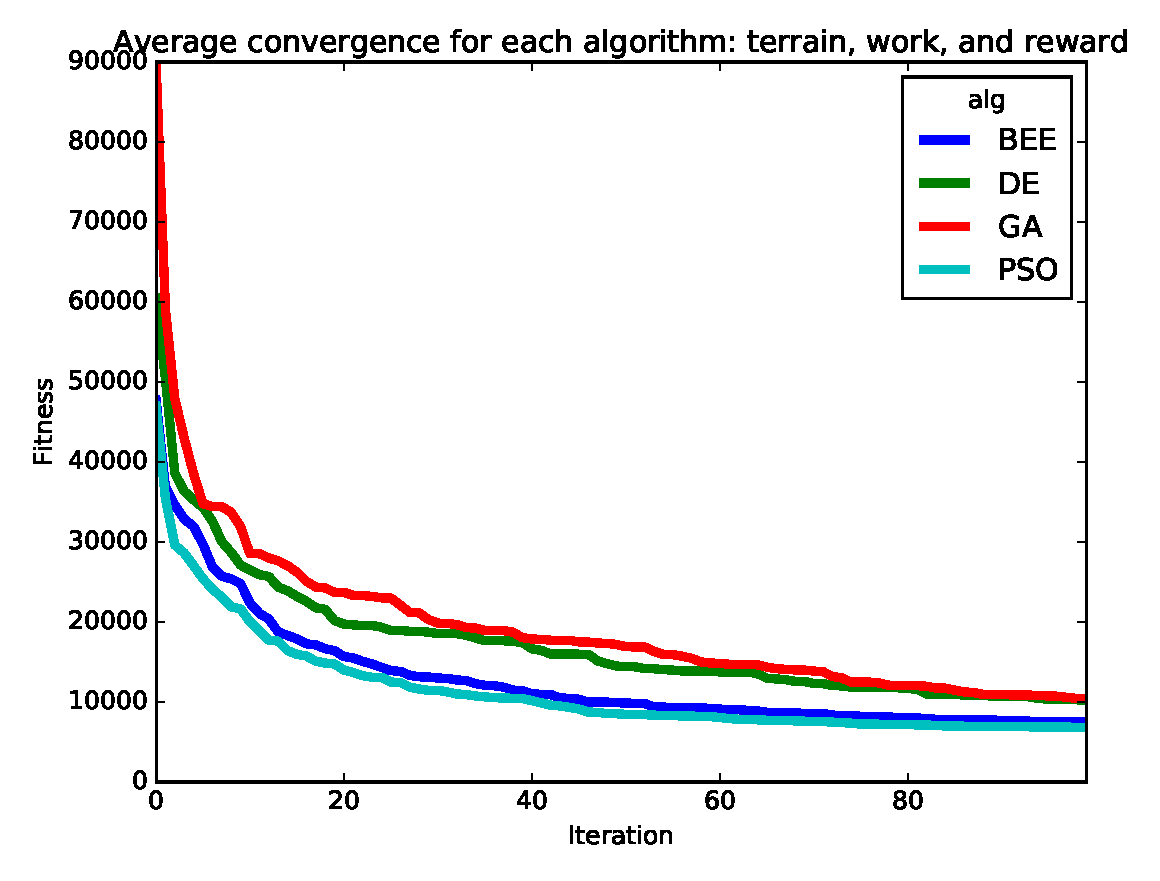
\includegraphics[width=0.75\textwidth,trim={0cm 0.75cm 0cm 0.75cm},clip]{conv_avg_b.eps}
    \caption{Average convergence for all algorithms, optimizing work and reward}
    \label{fig:convergence_b_avg}
\end{figure}

%%%%%%%%%%%%%%%%%%%%%%%%%%
% End convergence curves %
%%%%%%%%%%%%%%%%%%%%%%%%%%


%%%%%%%%%%%%%%%%%%%%%
% Algorithm compare %
%%%%%%%%%%%%%%%%%%%%%

\begin{figure}[H]
    \captionsetup{justification=centering}
    \centering
    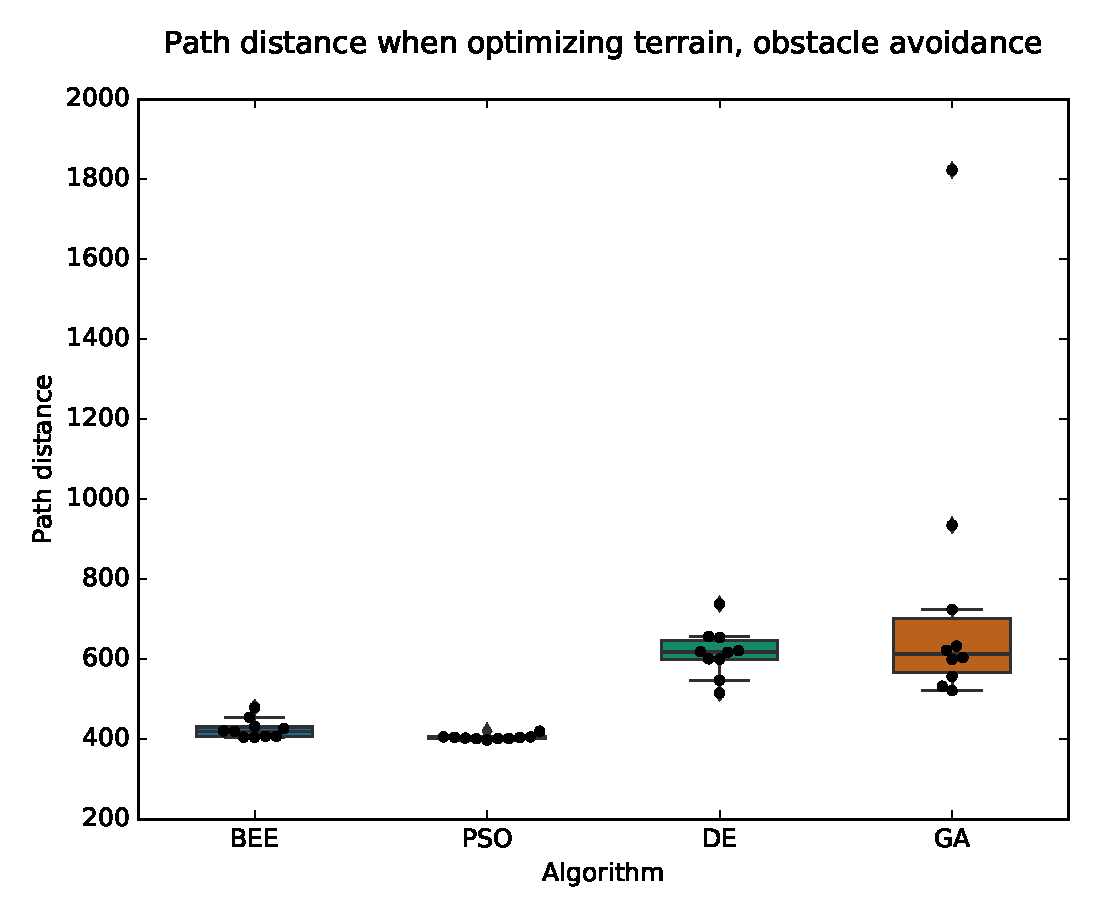
\includegraphics[width=0.75\textwidth,trim={0cm 0.75cm 0cm 0.75cm},clip]{EXP3_histo_distance_a.eps}
    \caption{\textit{Goto} path distance distribution. Not optimizing work and reward. }
    \label{fig:algcompare_a_distance}
\end{figure}

\begin{figure}[H]
    \captionsetup{justification=centering}
    \centering
    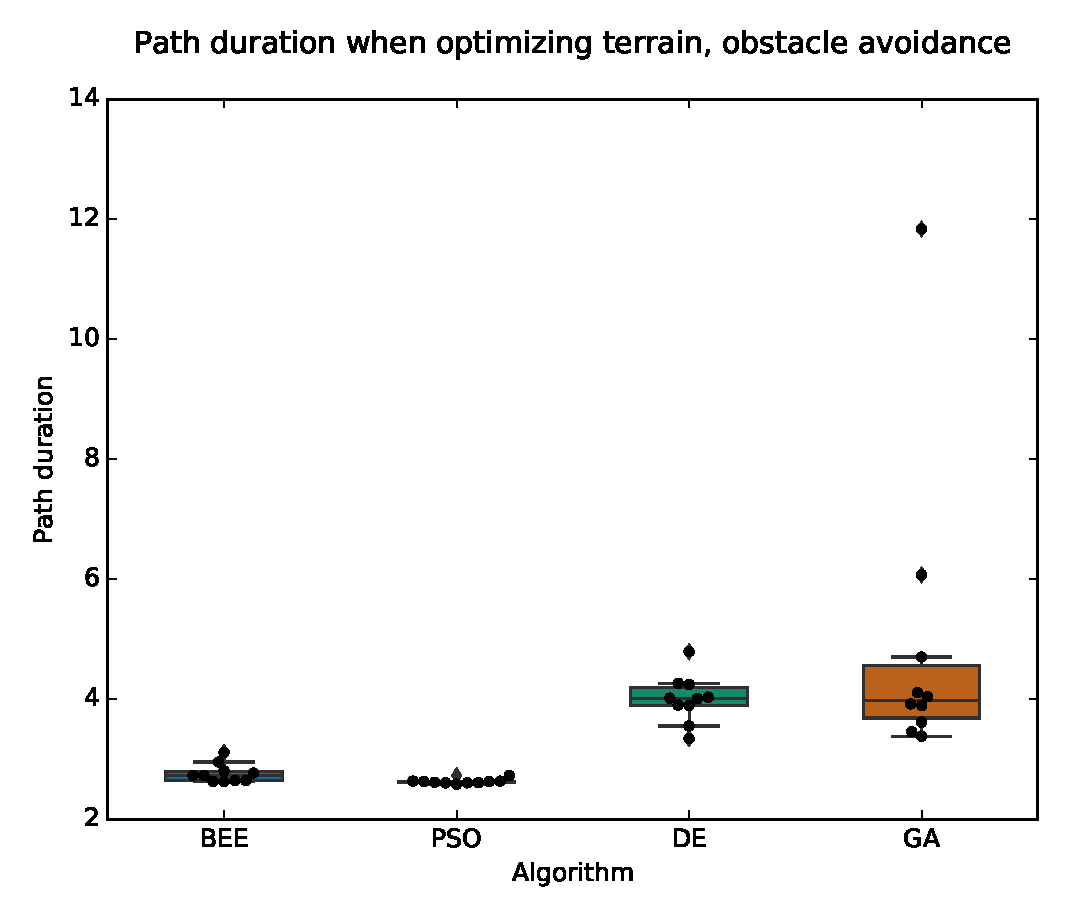
\includegraphics[width=0.75\textwidth,trim={0cm 0.75cm 0cm 0.75cm},clip]{EXP3_histo_duration_a.eps}
    \caption{\textit{Goto} path duration distribution. Not optimizing work and reward. }
    \label{fig:algcompare_a_duration}
\end{figure}

\begin{figure}[H]
    \captionsetup{justification=centering}
    \centering
    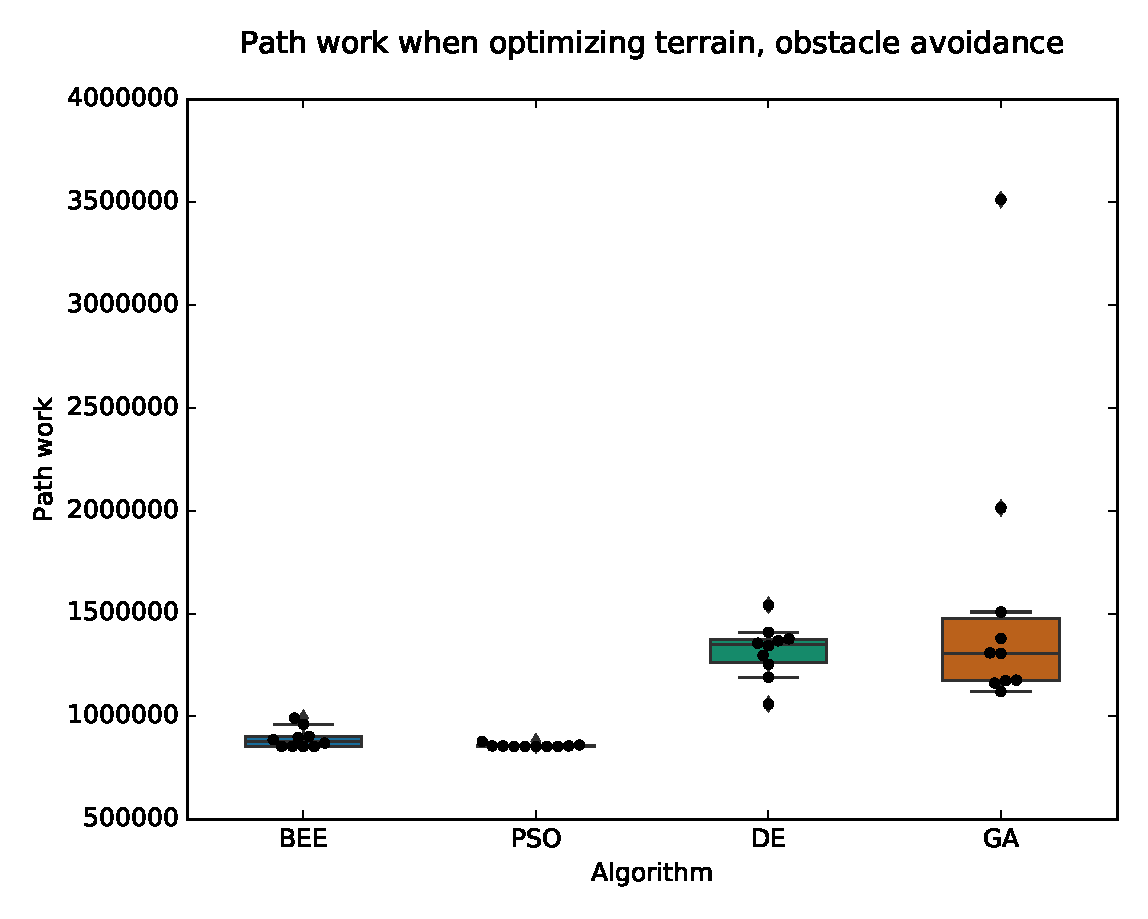
\includegraphics[width=0.75\textwidth,trim={0cm 0.75cm 0cm 0.75cm},clip]{EXP3_histo_work_a.eps}
    \caption{\textit{Goto} path work distribution. Not optimizing work and reward. }
    \label{fig:algcompare_a_work}
\end{figure}

\begin{figure}[H]
    \captionsetup{justification=centering}
    \centering
    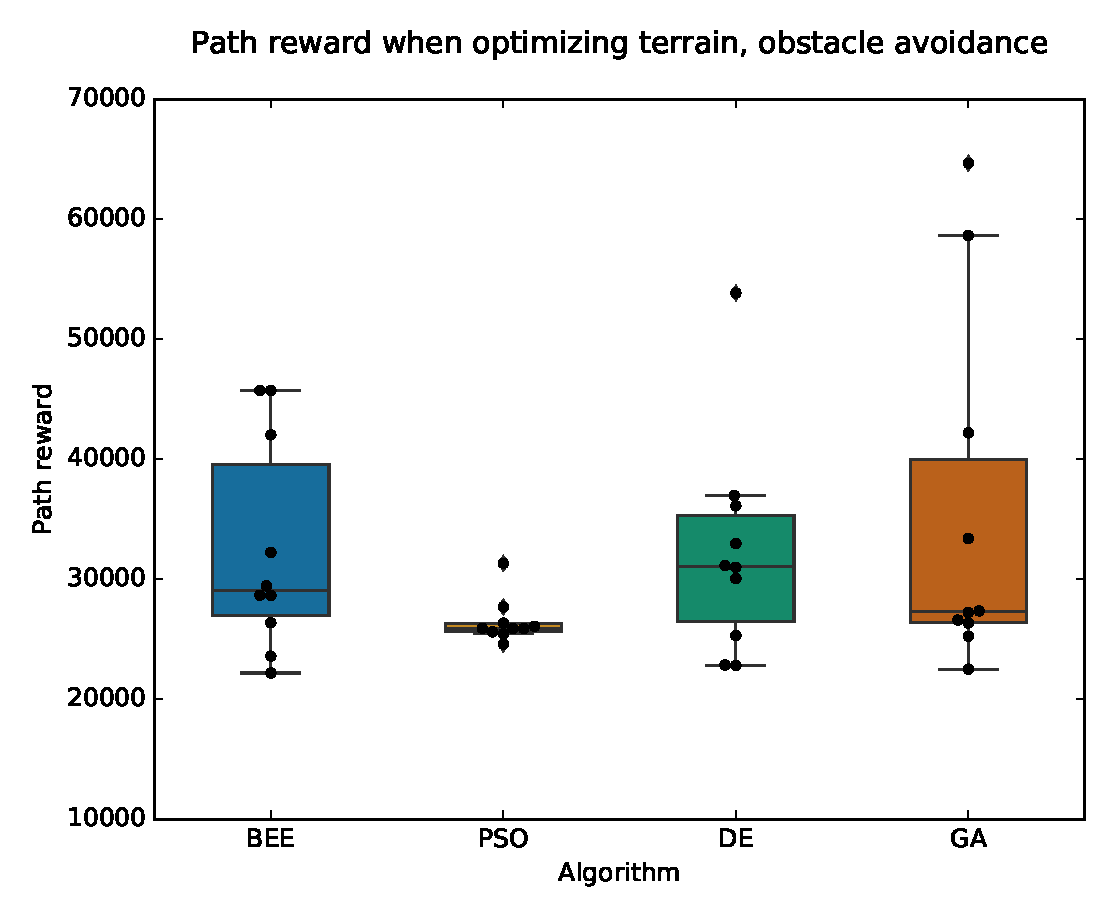
\includegraphics[width=0.75\textwidth,trim={0cm 0.75cm 0cm 0.75cm},clip]{EXP3_histo_reward_a.eps}
    \caption{\textit{Goto} path distance distribution. Optimizing work and reward. }
    \label{fig:algcompare_a_reward}
\end{figure}

\begin{figure}[H]
    \captionsetup{justification=centering}
    \centering
    \includegraphics[width=0.75\textwidth,trim={0cm 0.75cm 0cm 0.75cm},clip]{EXP3_histo_distance_b.eps}
    \caption{\textit{Goto} path duration distribution. Optimizing work and reward. }
    \label{fig:algcompare_b_distance}
\end{figure}

\begin{figure}[H]
    \captionsetup{justification=centering}
    \centering
    \includegraphics[width=0.75\textwidth,trim={0cm 0.75cm 0cm 0.75cm},clip]{EXP3_histo_duration_b.eps}
    \caption{\textit{Goto} path work distribution. Optimizing work and reward. }
    \label{fig:algcompare_b_duration}
\end{figure}

\begin{figure}[H]
    \captionsetup{justification=centering}
    \centering
    \includegraphics[width=0.75\textwidth,trim={0cm 0.75cm 0cm 0.75cm},clip]{EXP3_histo_work_b.eps}
    \caption{\textit{Goto} path reward distribution. Optimizing work and reward. }
    \label{fig:algcompare_b_work}
\end{figure}

\begin{figure}[H]
    \captionsetup{justification=centering}
    \centering
    \includegraphics[width=0.75\textwidth,trim={0cm 0.75cm 0cm 0.75cm},clip]{EXP3_histo_reward_b.eps}
    \caption{\textit{Goto} path reward distribution. Not optimizing work and reward. }
    \label{fig:algcompare_b_reward}
\end{figure}

%%%%%%%%%%%%%%%%%%%%%%%%%
% End algorithm compare %
%%%%%%%%%%%%%%%%%%%%%%%%%

The system should be able to influence path planning to achieve a desired planning behavior. This means that settings should be set that can make the planner more oriented around efficient travel or more interested in collecting opportunistic rewards. Optimization weights must be able to be manipulated such that they achieve this effect, and the weights should transfer to other situations. In other words, the is not useful if the weights have to be tuned for each path. If a set of weights emphasis reward for one scenario, it should do so for most, if not all, scenarios. In the following, the weights are tuned to see if the \textit{Surveyor} can be made to emphasis efficiency, reward, and a balance of both. Given the large scale of the environments, subtle deviations for increasing the reward are desired but should avoid going far off course. The exact bounds of what defines too far is subjective and application-specific, but the follows gives a sense of what is possible. 

Several random pairs of weights are generated to find the desired behavior: opportunistic-but-largely-efficient path planning. Meaning, additional work and/or reward optimization occurs such that opportunities for extra reward are taken advantage of but without dramatically harming efficiency. Four illustrative sets of weights are shown in Table \ref{tbl:weight_sets}, followed by images of runs using them. Sets $S^a$ and $S^b$ show behavior that meet the planning criteria; $S^b$ will be shown to be the better of the two. For comparison, $S^c$ and $S^d$ yield paths that collect much more reward but at massive loss of efficiency. These paths are not suitable, as discussed. 


% Weight sets S^a, S^b, S^c, S^d
\begin{table}[H]
    \begin{tabular}{|l|l|l|l|l|}
        \hline
        Weight set & $W_{work}$ & $W_{reward}$ & Comment & Figure \\
        \hline
        $S^a$ & 0.001 & 0.001 & Efficient, with some reward & Figure \ref{fig:weights_Sa} \\
        \hline
        $S^b$ & 0.01 & 0.005 & More efficient \& more reward than $S^a$ & Figure \ref{fig:weights_Sb} \\
        \hline
        $S^c$ & 0.00001 & 0.01 & Increased reward $\rightarrow$ massively inefficient & Figure \ref{fig:weights_Sc} \\
        \hline
        $S^d$ & 0.001 & 0.01 & Increased reward $\rightarrow$ massively inefficient & Figure \ref{fig:weights_Sd} \\
        \hline
    \end{tabular}
    \caption{Randomly chosen pairs of weight and their overall planning behavior.}
    \label{tbl:weight_sets}
\end{table}

Weight sets $S^a$ and $S^b$ are compared in Table \ref{tbl:weight_compare_a_b}. Visually, it is hard to determine which is weights perform better; both are reasonably close to the distance-only optimization to image that they are collecting rewards appropriately. The path attributes (duration, work, and reward) are required to fully characterize the behavior of these weights. A comparison of $S^a$ and $S^b$ is given in Table \ref{tbl:weightDiff_a_b}. The desired path planning is that reward optimization is present but without substantially deviating from an efficient path. Unfortunately, this is subjective but it is possible to identify scenarios where one set of weights performed better than another. In this case, $S^b$ can reasonably be said to outperform $S^c$. It is reported here, since was the best out of a number of sets randomly tried. Consider first the reward. In all cases, the reward using $S^b$, $S^b_{reward}$, is either greater than $S^a$ or approximately equivalent. In the worst case, the reward is 0.03 less than using $S^a$ for the same \textit{Goto} task. In the best case, it collects $61\%$ more reward than $S^a$. The ability to collect reward without major efficient loss is dependent on the availability of nearby reward or located such that water currents can be taken advantage of to reach them. So, there will be paths where the reward is stable even when the weight on reward is higher. This is the case for \textit{Goto} task 1-B, where there is no significant change in duration, work, or reward. This is better than the planner's reward maximization forcing it to go too far off course. But there are also situations that display dramatic increase in the reward with minimal impact on efficiency. This is the case for \textit{Goto} task 3-A: the $61\%$ reward increase occurred while actually improving duration and work. In order to clarify how these percentages reflect differences between path behavior, see Table \ref{tbl:weightDiff_d_b} for a comparison of $S^b$ with the highly inefficient $S^d$. While it has to be acknowledged that an objective assertion of the best sets of weights is difficult and application-specific, it can be said that the behavior observed using $S^b$ (among other weight pairs) enables the exact \textit{Goto} pat planning that the author envisioned for this system. 

These initial results are used to define an algorithm for automatically tuning weights given constraints. The constraint is the percent that the path is allowed to deviate from the path made if reward is not being maximized. The percent is a manually-set tolerance that represents the user's specification of \textit{desired path behavior}, a concept that was previously undefined in this text. The \textit{Surveyor}, through experimenting with a range of weights, is responsible for finding the weights that meet the criteria. Path planning is done with the work and reward criteria disabled, leaving just the obstacle-free minimized distance path. This is used a baseline. The \textit{Surveyor} then adds in work and reward weights over a range with some interval (smaller intervals increase the number of \textit{Goto} invocations but allow finer tuning). The weights whose path gives the best reward within constraints is selected. The critical element is that the \textit{Surveyor} does not tune wieghts for each path, as tuning involves several \textit{Goto} invocations. Instead the weights selected should be used for multiple paths. The results observed suggest that it is reasonable to do so. If it is discovered that sufficient differences in the environment cause the path planning to stray from the desired behavior (exceed constraints), then perhaps environments may be classified into types that correspond to a set of learned weights. 

% Compare planning with weights S^a, S^b
\begin{table}[H]
    \begin{tabular}{|l|l|l|l|}
        \hline
        Goto task & $S^a_{duration} \div S^b_{duration}$ & $S^a_{work} \div S^b_{work}$ & $S^a_{reward} \div S^b_{reward}$ \\
        \hline
        1-A & 1.11 & 1.17 & 0.89 \\
        \hline
        1-B & 1.03 & 1.02 & 1.03 \\
        \hline
        2-A & 0.96 & 1.00 & 0.93 \\
        \hline
        2-B & 1.03 & 1.13 & 1.02 \\
        \hline
        3-A & 1.16 & 1.18 & 0.39 \\
        \hline
        3-B &  1.15 & 1.13 & 0.91 \\
        \hline
    \end{tabular}
    \caption[Varying optimization criteria weights, weight sets $S^a$ and $S^b$.]{Comparison of duration, work, reward between weight sets $S^a = (W_{work} = 0.001$, $W_{reward} = 0.001)$ and $S^b = (W_{work} = 0.01$, $W_{reward} = 0.005)$.}
    \label{tbl:weightDiff_a_b}
\end{table}

% Compare planning with weights S^d, s^b
\begin{table}[H]
    \begin{tabular}{|l|l|l|l|}
        \hline
        Goto task & $S^d_{duration} \div S^b_{duration} (minutes)$ & $S^d_{work} \div S^b_{work}$ & $S^d_{reward} \div S^b_{reward}$ \\
        \hline
        1-A & 5.74 & 6.50 & 8.16 \\
        \hline
        1-B & 4.83 & 5.75 & 4.12 \\
        \hline
        2-A & 6.76 & 7.96 & 3.93 \\
        \hline
        2-B & 5.17 & 6.29 & 3.23 \\
        \hline
        3-A & 2.43 & 2.80 & 2.31 \\
        \hline
        3-B & 2.91 & 4.06 & 2.59 \\
        \hline
    \end{tabular}
    \caption[Varying optimization criteria weights, weight sets $S^d$ and $S^b$.]{Comparison of duration, work, reward between weight sets $S^d = (W_{work} = 0.001$, $W_{reward} = 0.01)$ and $S^a = (W_{work} = 0.01$, $W_{reward} = 0.005)$.}
    \label{tbl:weightDiff_d_b}
\end{table}

% Weights investigation: Sa
\begin{figure}[H]
    \centering
    \begin{subfigure}[b]{0.24\textwidth}
        \centering
        \includegraphics[width=\textwidth,trim={4cm 3cm 2cm 3cm},clip]{EXP3RG_PathAa_-1_-1_0d001_0.png}
        \caption{{\small Task 1-A \\ $W_{current}$: 0.001 \\ $W_{reward}$: 0}}    
        \label{fig:Path_1-A_upCurrent_noReward}
    \end{subfigure}
    \begin{subfigure}[b]{0.24\textwidth}  
        \centering 
        \includegraphics[width=\textwidth,trim={4cm 3cm 2cm 3cm},clip]{EXP3RG_PathAa_-1_-1_0d001_-1.png}
        \caption{{\small Task 1-A \\ $W_{current}$: 0.001 \\ $W_{reward}$: 0.001}}
        \label{fig:Path_1-A_upCurrent_Reward}
    \end{subfigure}
    \begin{subfigure}[b]{0.24\textwidth}
        \centering
        \includegraphics[width=\textwidth,trim={4cm 3cm 2cm 3cm},clip]{EXP3RG_PathAb_-1_-1_0d001_0.png}
        \caption{{\small Task 1-B \\ $W_{current}$: 0.001 \\ $W_{reward}$: 0}}
        \label{fig:Path_1-B_upCurrent_noReward}
    \end{subfigure}
    \begin{subfigure}[b]{0.24\textwidth}  
        \centering 
        \includegraphics[width=\textwidth,trim={4cm 3cm 2cm 3cm},clip]{EXP3RG_PathAb_-1_-1_0d001_-1.png}
        \caption{{\small Task 1-B \\ $W_{current}$: 0.001 \\ $W_{reward}$: 0.001}}
        \label{fig:Path_1-B_upCurrent_Reward}
    \end{subfigure}
    
    \vskip\baselineskip  
        
    \begin{subfigure}[b]{0.24\textwidth}
        \centering
        \includegraphics[width=\textwidth,trim={4cm 3cm 2cm 3cm},clip]{EXP3RG_PathBa_-1_-1_0d001_0.png}
        \caption{{\small Task 2-A \\ $W_{current}$: 0.001 \\ $W_{reward}$: 0}}    
        \label{fig:Path_2-A_upCurrent_noReward}
    \end{subfigure}
    \begin{subfigure}[b]{0.24\textwidth}  
        \centering 
        \includegraphics[width=\textwidth,trim={4cm 3cm 2cm 3cm},clip]{EXP3RG_PathBa_-1_-1_0d001_-1.png}
        \caption{{\small Task 2-A \\ $W_{current}$: 0.001 \\ $W_{reward}$: 0.001}}   
        \label{fig:Path_2-A_upCurrent_Reward}
    \end{subfigure}
  \begin{subfigure}[b]{0.24\textwidth}
        \centering
        \includegraphics[width=\textwidth,trim={4cm 3cm 2cm 3cm},clip]{EXP3RG_PathBb_-1_-1_0d001_0.png}
        \caption{{\small Task 2-B \\ $W_{current}$: 0.001 \\ $W_{reward}$: 0}}    
        \label{fig:Path_2-B_upCurrent_noReward}
    \end{subfigure}
    \begin{subfigure}[b]{0.24\textwidth}  
        \centering 
        \includegraphics[width=\textwidth,trim={4cm 3cm 2cm 3cm},clip]{EXP3RG_PathBb_-1_-1_0d001_-1.png}
        \caption{{\small Task 2-B \\ $W_{current}$: 0.001 \\ $W_{reward}$: 0.001}}   
        \label{fig:Path_2-B_upCurrent_Reward}
    \end{subfigure}
    
    \vskip\baselineskip       

    \begin{subfigure}[b]{0.24\textwidth}
        \centering
        \includegraphics[width=\textwidth,trim={4cm 3cm 2cm 3cm},clip]{EXP3RG_PathCa_-1_-1_0d001_0.png}
        \caption{{\small Task 3-A \\ $W_{current}$: 0.001 \\ $W_{reward}$: 0}}    
        \label{fig:Path_3-A_upCurrent_noReward}
    \end{subfigure}
    \begin{subfigure}[b]{0.24\textwidth}  
        \centering 
        \includegraphics[width=\textwidth,trim={4cm 3cm 2cm 3cm},clip]{EXP3RG_PathCa_-1_-1_0d001_-1.png}
        \caption{{\small Task 3-A \\ $W_{current}$: 0.001 \\ $W_{reward}$: 0.001}}   
        \label{fig:Path_3-A_upCurrent_Reward}
    \end{subfigure}
    \begin{subfigure}[b]{0.24\textwidth}
        \centering
        \includegraphics[width=\textwidth,trim={4cm 3cm 2cm 3cm},clip]{EXP3RG_PathCb_-1_-1_0d001_0.png}
        \caption{{\small Task 3-B \\ $W_{current}$: 0.001 \\ $W_{reward}$: 0}}    
        \label{fig:Path_3-B_upCurrent_noReward}
    \end{subfigure}
    \begin{subfigure}[b]{0.24\textwidth}  
        \centering 
        \includegraphics[width=\textwidth,trim={4cm 3cm 2cm 3cm},clip]{EXP3RG_PathCb_-1_-1_0d001_-1.png}
        \caption{{\small Task 3-B \\ $W_{current}$: 0.001 \\ $W_{reward}$: 0.001}}   
        \label{fig:Path_3-B_upCurrent_Reward}
    \end{subfigure}
    \caption[Solutions for Goto tasks using weights $S^a$.]{Solutions for Goto tasks, $S^a = (W_{work} = 0.001$, $W_{reward} = 0.001)$. \\ (With and without setting $W_{reward} = 0$).}
    \label{fig:weights_Sa}
\end{figure}

% Weights investigation: Sb
\begin{figure}[H]
    \centering
    \begin{subfigure}[b]{0.24\textwidth}
        \centering
            \includegraphics[width=\textwidth,trim={4cm 3cm 2cm 3cm},clip]{EXP3RG_PathAa_-1_-1_0d01_0d005.png}
        \caption{Path 1-A }    
        \label{fig:Path_1-A_upReward_upWork_b}
    \end{subfigure}
    %\hfill
    \begin{subfigure}[b]{0.24\textwidth}  
        \centering 
        \includegraphics[width=\textwidth,trim={4cm 3cm 2cm 3cm},clip]{EXP3RG_PathBa_-1_-1_0d01_0d005.png}
        \caption{Path 2-A}
        \label{fig:Path_2-A_upReward_upWork_b}
    \end{subfigure}
    %\hfill
    \begin{subfigure}[b]{0.24\textwidth}
        \centering
        \includegraphics[width=\textwidth,trim={4cm 3cm 2cm 3cm},clip]{EXP3RG_PathBa_-1_-1_0d01_0d005.png}
        \caption{Path 3-A}
        \label{fig:Path_3-A_upReward_upWork_b}
    \end{subfigure}
    \vskip\baselineskip  
    \begin{subfigure}[b]{0.24\textwidth}
        \centering
        \includegraphics[width=\textwidth,trim={4cm 3cm 2cm 3cm},clip]{EXP3RG_PathAb_-1_-1_0d01_0d005.png}
        \caption{Path 1-B}    
        \label{fig:Path_1-B_upReward_upWork_b}
    \end{subfigure}
    \begin{subfigure}[b]{0.24\textwidth}  
        \centering 
        \includegraphics[width=\textwidth,trim={4cm 3cm 2cm 3cm},clip]{EXP3RG_PathBb_-1_-1_0d01_0d005.png}
        \caption{Path 2-B}   
        \label{fig:Path_2-B_upReward_upWork_b}
    \end{subfigure}
  \begin{subfigure}[b]{0.24\textwidth}
        \centering
        \includegraphics[width=\textwidth,trim={4cm 3cm 2cm 3cm},clip]{EXP3RG_PathCb_-1_-1_0d01_0d005.png}
        \caption{Path 3-B}    
        \label{fig:Path_3-B_upReward_upWork_b}
    \end{subfigure}
    \caption[Solutions for Goto tasks using weights $S^b$.]{Solutions for Goto tasks, $S^b = (W_{work} = 0.01$, $W_{reward} = 0.005)$.}
    \label{fig:weights_Sb}
\end{figure}

% Weights investigation: Sc
\begin{figure}[H]
    \centering
    \begin{subfigure}[b]{0.24\textwidth}
        \centering
            \includegraphics[width=\textwidth,trim={4cm 3cm 2cm 3cm},clip]{EXP3RG_PathAa_-1_-1_0_0d01.png}
        \caption{{\small Path 1-A \\ $W_{current}$: 0 \\ $W_{reward}$: 0.01}}    
        \label{fig:Path_1-A_upReward_noWork}
    \end{subfigure}
    \begin{subfigure}[b]{0.24\textwidth}  
        \centering 
        \includegraphics[width=\textwidth,trim={4cm 3cm 2cm 3cm},clip]{EXP3RG_PathAa_-1_-1_-1_0d01.png}
        \caption{{\small Path 1-A \\ $W_{current}$: 0.00001 \\ $W_{reward}$: 0.01}}
        \label{fig:Path_1-A_upReward_Work}
    \end{subfigure}
    \begin{subfigure}[b]{0.24\textwidth}
        \centering
        \includegraphics[width=\textwidth,trim={4cm 3cm 2cm 3cm},clip]{EXP3RG_PathAb_-1_-1_0_0d01.png}
        \caption{{\small Path 1-B \\ $W_{current}$: 0 \\ $W_{reward}$: 0.01}}
        \label{fig:Path_1-B_upReward_noWork}
    \end{subfigure}
    \begin{subfigure}[b]{0.24\textwidth}  
        \centering 
        \includegraphics[width=\textwidth,trim={4cm 3cm 2cm 3cm},clip]{EXP3RG_PathAb_-1_-1_-1_0d01.png}
        \caption{{\small Path 1-B \\ $W_{current}$: 0.00001 \\ $W_{reward}$: 0.01}}
        \label{fig:Path_1-B_upReward_Work}
    \end{subfigure}
    \vskip\baselineskip  
    \begin{subfigure}[b]{0.24\textwidth}
        \centering
        \includegraphics[width=\textwidth,trim={4cm 3cm 2cm 3cm},clip]{EXP3RG_PathBa_-1_-1_0_0d01.png}
        \caption{{\small Path 2-A \\ $W_{current}$: 0 \\ $W_{reward}$: 0.01}}    
        \label{fig:Path_2-A_upReward_noWork}
    \end{subfigure}
    \begin{subfigure}[b]{0.24\textwidth}  
        \centering 
        \includegraphics[width=\textwidth,trim={4cm 3cm 2cm 3cm},clip]{EXP3RG_PathBa_-1_-1_-1_0d01.png}
        \caption{{\small Path 2-A \\ $W_{current}$: 0.00001 \\ $W_{reward}$: 0.01}}   
        \label{fig:Path_2-A_upReward_Work}
    \end{subfigure}
  \begin{subfigure}[b]{0.24\textwidth}
        \centering
        \includegraphics[width=\textwidth,trim={4cm 3cm 2cm 3cm},clip]{EXP3RG_PathBb_-1_-1_0_0d01.png}
        \caption{{\small Path 2-B \\ $W_{current}$: 0 \\ $W_{reward}$: 0.01}}    
        \label{fig:Path_2-B_upReward_noWork}
    \end{subfigure}
    \begin{subfigure}[b]{0.24\textwidth}  
        \centering 
        \includegraphics[width=\textwidth,trim={4cm 3cm 2cm 3cm},clip]{EXP3RG_PathBb_-1_-1_-1_0d01.png}
        \caption{{\small Path 2-B \\ $W_{current}$: 0.00001 \\ $W_{reward}$: 0.01}}   
        \label{fig:Path_2-B_upReward_Work}
    \end{subfigure}
    \vskip\baselineskip      
    \begin{subfigure}[b]{0.24\textwidth}
        \centering
            \includegraphics[width=\textwidth,trim={4cm 3cm 2cm 3cm},clip]{EXP3RG_PathCa_-1_-1_0_0d01.png}
        \caption{{\small Path 3-A \\ $W_{current}$: 0 \\ $W_{reward}$: 0.01}}    
        \label{fig:Path_3-A_upReward_noWork}
    \end{subfigure}
    \begin{subfigure}[b]{0.24\textwidth}  
        \centering 
        \includegraphics[width=\textwidth,trim={4cm 3cm 2cm 3cm},clip]{EXP3RG_PathCa_-1_-1_-1_0d01.png}
        \caption{{\small Path 3-A \\ $W_{current}$: 0.00001 \\ $W_{reward}$: 0.01}}   
        \label{fig:Path_3-A_upReward_Work}
    \end{subfigure}
    \begin{subfigure}[b]{0.24\textwidth}
        \centering
        \includegraphics[width=\textwidth,trim={4cm 3cm 2cm 3cm},clip]{EXP3RG_PathCb_-1_-1_0_0d01.png}
        \caption{{\small Path 3-B \\ $W_{current}$: 0 \\ $W_{reward}$: 0.01}}    
        \label{fig:Path_3-B_upReward_noWork}
    \end{subfigure}
    \begin{subfigure}[b]{0.24\textwidth}  
        \centering 
        \includegraphics[width=\textwidth,trim={4cm 3cm 2cm 3cm},clip]{EXP3RG_PathCb_-1_-1_-1_0d01.png}
        \caption{{\small Path 3-B \\ $W_{current}$: 0.00001 \\ $W_{reward}$: 0.01}}   
        \label{fig:Path_3-B_upReward_Work}
    \end{subfigure}
    \caption[Solutions for Goto tasks using weights $S^c$.]{Solutions for Goto tasks, $S^c = (W_{work} = 0.00001$, $W_{reward} = 0.01)$. \\ (With and without setting $W_{reward} = 0$).}
    \label{fig:weights_Sc}
\end{figure}

% Weights investigation Sd
\begin{figure}[H]
    \centering
    \begin{subfigure}[b]{0.24\textwidth}
        \centering
            \includegraphics[width=\textwidth,trim={4cm 3cm 2cm 3cm},clip]{EXP3RG_PathAa_-1_-1_0d001_0d01.png}
        \caption{Path 1-A}    
        \label{fig:Path_1-A_upReward_upWork}
    \end{subfigure}
    \begin{subfigure}[b]{0.24\textwidth}  
        \centering 
        \includegraphics[width=\textwidth,trim={4cm 3cm 2cm 3cm},clip]{EXP3RG_PathBa_-1_-1_0d001_0d01.png}
        \caption{Path 2-A}
        \label{fig:Path_2-A_upReward_upWork}
    \end{subfigure}
    \begin{subfigure}[b]{0.24\textwidth}
        \centering
        \includegraphics[width=\textwidth,trim={4cm 3cm 2cm 3cm},clip]{EXP3RG_PathBa_-1_-1_0d001_0d01.png}
        \caption{Path 2-A}
        \label{fig:Path_3-A_upReward_upWork}
    \end{subfigure}
    \vskip\baselineskip  
    \begin{subfigure}[b]{0.24\textwidth}
        \centering
        \includegraphics[width=\textwidth,trim={4cm 3cm 2cm 3cm},clip]{EXP3RG_PathAb_-1_-1_0d001_0d01.png}
        \caption{Path 1-B}    
        \label{fig:Path_1-B_upReward_upWork}
    \end{subfigure}
    \begin{subfigure}[b]{0.24\textwidth}  
        \centering 
        \includegraphics[width=\textwidth,trim={4cm 3cm 2cm 3cm},clip]{EXP3RG_PathBb_-1_-1_0d001_0d01.png}
        \caption{Path 2-B}   
        \label{fig:Path_2-B_upReward_upWork}
    \end{subfigure}
  \begin{subfigure}[b]{0.24\textwidth}
        \centering
        \includegraphics[width=\textwidth,trim={4cm 3cm 2cm 3cm},clip]{EXP3RG_PathCb_-1_-1_0d001_0d01.png}
        \caption{Path 3-B}
        \label{fig:Path_3-B_upReward_upWork}
    \end{subfigure}
    \vskip\baselineskip       
    \caption[Solutions for Goto tasks using weights $S^d$.]{Solutions for Goto tasks, $S^d = (W_{work} = 0.011$, $W_{reward} = 0.01)$.}
    \label{fig:weights_Sd}
\end{figure}

\section{Coverage Planner}

The \textit{Coverage} planner implemented is a trivial lawnmower path over obstacle-free regions. An analysis of the performance is not interesting, since planning algorithms exist more suited to USV dynamics and that incorporate obstacle avoidance. The appeal of the lawnmower planner is that is computes in seconds and is not tailored for a particular vehicle. These results are used to investigate the impact of water currents on planning and usefulness of using a set of forecasts rather than a single current estimate. The 5 regions are shown in Figure \ref{fig:env_targets} and listed in Table \ref{tbl:env_targets}. The Lawnmower \textit{Coverage} planner generates row-wise and column-wise traversal of each cell in the region, measures the work required by each, and selects the more efficient. Here, the results of both row-wise and column-wise were collected for comparison. Recall that each band of the magnitude and direction current rasters correspond to a 30-minute interval. A duration estimate accumulates during evaluation of the fitness function in order to choose appropriate band. Work estimates are measured for each of the regions, as shown in Table \ref{tbl:coverage_work_measures}. 

Experimental results are summarized in Tables \ref{tbl:coverage_work_measures} and \ref{tbl:coverage_work_diff_measures}. $R_1$ (Figure \ref{fig:coverage_noterrain_work_r1}, \ref{fig:coverage_noterrain_diff_r1}) is so small that there is little room for the water currents to make an appreciable effect. The region is covered in under 30 minutes, so water currents stay in a single interval. The row-wise movement is slightly less than column-wise. $R_2$ (Figure \ref{fig:coverage_noterrain_work_r2}, \ref{fig:coverage_noterrain_diff_r2}) has greater aread than $R_1$ and is much more sensitive to the choice of movement scheme: row-wise work is ( NUM \%) of columnwise. Time become applicable in $R_3$ (Figure \ref{fig:coverage_noterrain_work_r3}, \ref{fig:coverage_noterrain_diff_r3}), where three forecasts were used. The column-wise work remains stable, but the row-wise work drops significantly when updates are used. In $R_4$ (Figure \ref{fig:coverage_noterrain_work_r4}, \ref{fig:coverage_noterrain_diff_r4}), there is a large difference in work when using updates. Without updates, column-wise has better performance. With update, it switches to row-wise. The updates not only gave a better work estimate that will help the overall mission planner be more effective; they also changed the \textit{Coverage} plan. This is also seen in $R_5$ (Figure \ref{fig:coverage_noterrain_work_r4}, \ref{fig:coverage_noterrain_diff_r4}), where the 9 updates used help the path planner to select row-wise over column-wise. In these five example, the impact that water current updates (even as sparse as every 30 minutes) is made clear. Higher resolution update intervals are possible, but increase the time to generate the forecast data set from online sources. The optimal update resolution, balancing time and storage with work estimation accuracy, requires investigation.

\begin{table}[H]\small
    \begin{tabular}{|l|l|l|l|l|l|l|l|l|l|l|}
    \hline
 \thead{Region} & \thead{Region size \\ (meters)} & \thead{Region size \\ (cells)} & \thead{Distance \\ (cells)} & \thead{Duration \\ (minutes)} & \thead{Reward} & \thead{Current updates}  \\
\hline
1 & 1450 & 10 x 10 & 118.246 & 0.768 & 10643.620           & 0 \\
\hline
2 & 36250  & 50 x 50 & 2598.042 & 16.870 & 407659.374      & 0 \\
\hline
3 & 145000 & 100 x 100 & 10198.020 & 66.221 & 1030030.385  & 3 \\
\hline
4 & 326250 & 150 x 150 & 22798.014 & 148.039 & 1926660.004 & 5 \\
\hline
5 & 580000 & 200 x 200 & 40398.010 & 262.325 & 3520605.632 & 9 \\
\hline
    \end{tabular}
    \caption[Selected targets and their coverage regions.]{Selected targets and their coverage regions.}
    \label{tbl:env_targets}
\end{table}


\begin{table}[H]\small
    \begin{tabular}{|l|l|l|l|l|}
    \hline
        \thead{Region} & \thead{Work columnwise \\ (with updates)} & \thead{Work rowwise \\ (with updates)}  & \thead{Work columnwise \\ (no updates} & \thead{Work rowwise \\ (no updates)} \\
        \hline 
        $R_1$ &    513465.892 &    513452.073 & 513465.892 & 513452.073 &  \\
        \hline
        $R_2$ &  11903001.793 &  11890847.012 & 11903001.793 & 11890847.012 &   \\
        \hline
        $R_3$ &  47145978.158 &  47119054.520 & 47146078.734 & 47124199.557 &   \\
        \hline
        $R_4$ & 105728388.430 & 105685825.846 & 105704102.314 & 105728540.700  \\
        \hline
        $R_5$ & 187649992.045 & 187181080.951 & 187497561.286 & 187650706.827 \\
        \hline
    \end{tabular}
    \caption[Effect of movement scheme on work in \textit{Coverage} planning.]{Column-wise and row-wise work done in each region, with and without water current forecast updates.}
    \label{tbl:coverage_work_measures}
\end{table}


\begin{table}[H]\small
    \begin{tabular}{|l|l|l|l|}
    \hline
        \thead{Region} & \thead{Work difference \\ (with updates)} & \thead{Work difference \\ (no updates} & \thead{Difference of differences \\ (updates or not)}  \\
        \hline
        $R_1$ &     13.819 & 13.819    & 0 \\
        \hline
        $R_2$ &  12154.781 & 12154.781 & 0 \\
        \hline
        $R_3$ &  26923.638 & 21879.177 & 5044.461  \\
        \hline
        $R_4$ &  42562.584 & 24438.386 & 18124.198  \\
        \hline
        $R_5$ & 468911.094 & 153145.541 & 315765.553 \\
        \hline
    \end{tabular}
    \caption[Difference between movement schemes on work in \textit{Coverage} planning.]{The difference between column-wise and row-wise work, with and without updates}
    \label{tbl:coverage_work_diff_measures}
\end{table}


%%%%%%%%%%%%%%%%%%%%%%%%%
% Work coverage compare %
%%%%%%%%%%%%%%%%%%%%%%%%%
\begin{figure}[H]
    \captionsetup{justification=centering}
    \centering
    \includegraphics[width=\textwidth,trim={0cm 0cm 0cm 0.75cm},clip]{work_r1.eps}
    \caption{\textit{Coverage} path work in region 1.}
    \label{fig:coverage_noterrain_work_r1}
\end{figure}
\begin{figure}[H]
    \captionsetup{justification=centering}
    \centering
    \includegraphics[width=\textwidth,trim={0cm 0cm 0cm 0.75cm},clip]{diff_r1.eps}
    \caption{\textit{Coverage} path work in differences $R_1$.}
    \label{fig:coverage_noterrain_diff_r1}
\end{figure}

\begin{figure}[H]
    \captionsetup{justification=centering}
    \centering
    \includegraphics[width=\textwidth,trim={0cm 0cm 0cm 0.75cm},clip]{work_r2.eps}
    \caption{\textit{Coverage} path work in $R_2$.}
    \label{fig:coverage_noterrain_work_r2}
\end{figure}
\begin{figure}[H]
    \captionsetup{justification=centering}
    \centering
    \includegraphics[width=\textwidth,trim={0cm 0cm 0cm 0.75cm},clip]{diff_r2.eps}
    \caption{\textit{Coverage} path work in differences $R_2$.}
    \label{fig:coverage_noterrain_diff_r2}
\end{figure}

\begin{figure}[H]
    \captionsetup{justification=centering}
    \centering
    \includegraphics[width=\textwidth,trim={0cm 0cm 0cm 0.75cm},clip]{work_r3.eps}
    \caption{\textit{Coverage} path work in $R_3$.}
    \label{fig:coverage_noterrain_work_r3}
\end{figure}
\begin{figure}[H]
    \captionsetup{justification=centering}
    \centering
    \includegraphics[width=\textwidth,trim={0cm 0cm 0cm 0.75cm},clip]{diff_r3.eps}
    \caption{\textit{Coverage} path work differences in $R_3$.}
    \label{fig:coverage_noterrain_diff_r3}
\end{figure}

\begin{figure}[H]
    \captionsetup{justification=centering}
    \centering
    \includegraphics[width=\textwidth,trim={0cm 0cm 0cm 0.75cm},clip]{work_r4.eps}
    \caption{\textit{Coverage} path work in $R_4$.}
    \label{fig:coverage_noterrain_work_r4}
\end{figure}
\begin{figure}[H]
    \captionsetup{justification=centering}
    \centering
    \includegraphics[width=\textwidth,trim={0cm 0cm 0cm 0.75cm},clip]{diff_r4.eps}
    \caption{\textit{Coverage} path work differences in $R_4$.}
    \label{fig:coverage_noterrain_diff_r4}
\end{figure}

\begin{figure}[H]
    \captionsetup{justification=centering}
    \centering
    \includegraphics[width=\textwidth,trim={0cm 0cm 0cm 0.75cm},clip]{work_r5.eps}
    \caption{\textit{Coverage} path work in $R_5$.}
    \label{fig:coverage_noterrain_work_r5}
\end{figure}
\begin{figure}[H]
    \captionsetup{justification=centering}
    \centering
    \includegraphics[width=\textwidth,trim={0cm 0cm 0cm 0.75cm},clip]{diff_r5.eps}
    \caption{\textit{Coverage} path work differences in $R_5$.}
    \label{fig:coverage_noterrain_diff_r5}
\end{figure}

\subsection{Mission Planning}

Mission planning was performed for the targets in \ref{tbl:env_targets}, using both MPFC and MPTR. The maximum work and duration constraints were set high so that all targets could be visited. These targets were chosen with the intention of challenging the heuristics. An interesting situation is where the dynamic currents are such that the work varies depending on the elapsed duration when entering a planning segment or one where complex terrain makes the straight-line distance does not accurately estimate that actual distance required. 

% \begin{table}[H]\small
%     \begin{tabular}{|l|l|l|}
% \hline
% Situation & $D_{max} (minutes)$ & $W_{max} (Joules)$ \\
% \hline
% Visiting each target is feasible & 1000 & 10000000000 \\
% \hline  
% Visiting each target is infeasible &    & \\
% \hline
%     \end{tabular}
%     \caption[Mission planning experimental constraints.]{Constraints used in mission planning experiments.}
%     \label{tbl:constraints}
% \end{table}

\subsubsection{Mission Planning Fully-Connection}

MPFC evaluates every  possible path at great computational cost, even if accessing memoized results for the node sequence prefix. Unlike MPTR, the measurements of every mission are available for mission selection. Selection should be based on application goals, but at the mission planning level, efficiency is typically of greater concern. The vast majority of the reward is collected as part of the target coverage, so much of the reward is invariant between missions that reach all possible targets. The reward that varies is the opportunistic reward collecting during \textit{Goto} path planning. Because of the dynamic water currents effect on path planning, the opportunities to collect reward varies by the order in which nodes are visited. It is possible to prioritize reward maximization, since it is already established that these are feasible paths. But, these are estimates and the time could be spent better on additional targets or early arrival at the destination for safety concerns. Selection strategy could balance work and reward by, for example, finding a missions whose attributes are on the Pareto front. This approach allows finer-grained mission selection, but would be easier to answer if evaluation a non-simulated application. 

In deciding which attribute to base selection on, the path measurements are compared. Three missions are shown in Table \ref{tbl:MPFC_solutions}. These are missions where either the distance, work, or reward is at is best value (min or max as appropriate). Duration is proportional to distance and ignored. Figure \ref{fig:MPFC_box_withreward} shows how these missions compare to all the others. An immediate problem appears: the large width of candidate best solutions. The efficiency measurements are located within both the best and worst outliers. 

The reward width is actually not that massive: 200000 is large, but is less than half of what is achieved in region 2: the second smallest (see Figure \ref{fig:env_targets}). Meanwhile, the width of the duration is over an hour which means that it adds that much time when choosing best reward mission over the most efficient. Figure \ref{fig:MPFC_box_noreward} shows how the missions compare when not including the reward optimal as a candidate. The remaining two missions show a much tighter bound and are both in their outliers, which demonstrates the synergy in minimizers that both promote path efficiency. For this example system, the \textit{Surveyor} is set to select the feasible mission with the greatest number of targets that also has the minimum estimated work. In this case, the same route is chosen whether using distance or work. The top 5 missions, according to MPFC, are shown in Table \ref{tbl:MPFC_solutions_top5}. These are chosen whether using distance or work as the selection criteria.

\begin{table}[H]\small
    \begin{tabular}{|l|l|l|l|l|l|}
\hline
Node sequence & Optimized Attribute & Distance & Work & Reward \\
\hline
(0 1 5 2 3 4 6) & Reward   & 81489.301 & 3.637331e+08 & 7553974.458 \\
\hline
(0 1 3 2 5 4 6) & Work     & 78709.460 & 3.581165e+08 & 7399391.4482 \\
\hline
(0 1 3 2 5 4 6) & Distance & 78709.460 & 3.581165e+08  & 7399391.448 \\
\hline
    \end{tabular}
    \caption[Mission Planner Fully-Connected results.]{Missions found with MPFC that contain every target and have the best duration, work, or reward. Recall that duration is proportional to distance: work varies to maintain a constant speed.}
    \label{tbl:MPFC_solutions}
\end{table}

\begin{figure}[H]
    \captionsetup{justification=centering}
    \centering
    %\includegraphics[width=\textwidth,trim={0cm 0cm 0cm 0.75cm},clip]{diff_r4.eps}
    \includegraphics[width=\textwidth]{EXP4_MPFC_box_r.eps}
    \caption[Distribution of path attributes.]{Distribution of path attributes. Those labeled \textit{Has Best} include the missions where at least on path attribute is optimal. Those labeled \textit{No Best} have no optimal attribute.}
    \label{fig:MPFC_box_withreward}
\end{figure}

\begin{figure}[H]
    \captionsetup{justification=centering}
    \centering
    %\includegraphics[width=\textwidth,trim={0cm 0cm 0cm 0.75cm},clip]{diff_r4.eps}
    \includegraphics[width=\textwidth]{EXP4_MPFC_box_nr.eps}
    \caption[Distribution of path attributes, without reward in selecting best candidate solution.]{Distribution of path attributes. Those labeled \textit{Has Best} include the missions where at least on path attribute is optimal. Those labeled \textit{No Best} have no optimal attribute. Unlike Figure \ref{fig:MPFC_box_withreward}, the path with maximum reward is not included in \textit{Has Best}.}
    \label{fig:MPFC_box_noreward}
\end{figure}

\begin{table}[H]\small
    \begin{tabular}{|l|l|l|l|l|}
\hline
\thead{Route} & \thead{Distance \\ (MPFC)} & \thead{Duration \\ (MPFC)} & \thead{Work (MPFC)} & \thead{Reward (MPFC)} \\
\hline
(0 1 3 2 5 4 6)  &  78709.46 & 511.10 & 3.581165e+08 & 7399391.45 \\
\hline 
(0 1 2 5 3 4 6)  &  78930.23 & 512.53 & 3.584078e+08 & 7446916.43 \\
\hline
(0 5 4 3 2 1 6)  &  79155.94 & 514.00 & 3.587672e+08 & 7375456.17\\
\hline
(0 3 2 5 4 1 6)  &  79156.36 & 514.00 & 3.591452e+08 & 7422834.67 \\
\hline 
(0 1 4 5 2 3 6)  &  79280.62 & 514.81 & 3.593909e+08 & 7385970.29 \\
\hline 
    \end{tabular}
    \caption[MPFC: top 5 missions with respect to distance]{Mission Planner Fully-Connected: top 5 missions with respect to distance or work}
    \label{tbl:MPFC_solutions_top5}
\end{table}

These results will be used to guide the development of measurements for the heuristic mission planner MPTR. The goal is to find a method such that the chosen solution approaches the solution that would be chosen by MPFC. In other words, MPTR might choose a different mission but whose measurements are reasonably close to MPFC at a massive reduction in computing required. 

\subsubsection{Mission Planning Try \& Repair}

The top 5 missions selected using MPTR, with respect to distance, are shown in Table \ref{tbl:MPTR_solutions_top5_distance}. Using work, the top 5 missions are in Table \ref{tbl:MPTR_solutions_top5_work}. The immediate result is that the top mission chosen by MPTR does not match that of MPFC. This is not necessarily problematic since multiple missions could share very similar properties. However, that is not the case here. The difference between the two is 1969.78, whereas the difference between the top two MPFC choices is 190.15. To further illustrate the poor choice by MPTR, the difference between the MPC top choice and its fifth choice is still only 571.16. Note that these differences are calculated using the more accurate MPFC measurements. The top choice by MPTR is the 81st for MPFC. Interestingly, the second MPTR choice is the top MPFC choice; but with no way to determine this without also running MPFC, this does not help in selecting the best mission. There is the possibility that the second choice is a more accurate representation of the MPTR results and that the first is an outlier. This is not the case: of the top 5 MPTR choices, only the second appears within the top 5 MPFC. There is a complete lack of ability for MPTR measurements to predict MPFC. 

In an effort to salvage the result, an even more naive heuristic was tried. The goal was to show that MPTR's method at least improved upon using the straight-line euclidean distance between target region centers. The memoized \textit{Coverage} results were still used, but \textit{Goto} paths were replaced with this simple straight-line measurement; no consideration of terrain, currents, etc. The results are shown in Table \ref{tbl:straight_solutions_top5}. The result is not what was expected. The top result matches the top for MPFC. Unline MPTR, this is not simply a random outlier: $3/5$ of the top five using straight-line are in the top 5 MPFC. The worst of these is only 665.77 cells difference in distance from the top MPFC choice, which is only $33.80\%$ of the difference between the top choices for MPFC and MPTR. The straight-line distance is not perfect, but is a better predictor of the top MPFC missions that MPTR. Most importantly, MPTR still took ~5 hours, while this new version performed the entire mission planning in under a minute. 

Given this result, MPTR was updated to use the straight-line distance rather than the previously described system of \textit{Goto} invocation. Even though the latter considers the deviations from the straight line caused by obstacles, it is adversely affected by incomplete planning information. It is promising that decent results are obtained using trivial computations. It is easy to imagine scenarios where the complexity of the currents or terrain should make such a heuristic fail. More work is needed to find richer heuristics that can handle a wide variety of scenarios with relatively low computational footprint. Unlike the previous version of MPTR, the new formulation, using straight line distance heuristic, could be computed online. Even if additional experiments are not as effective, if this approach is able to typically provide good performance then it is a very good fit for online mission planning. 

\begin{table}[H]\small
    \begin{tabular}{|l|l|l|l|l|l|}
\hline
\thead{Route} & \thead{Distance \\ (MPTR)} & \thead{Distance \\ (MPFC)} & \thead{Work (MPTR)} & \thead{Work (MPFC)} & \thead{MPFC's $ith$ choice} \\
\hline
 (0 1 3 2 4 5 6) & 79127.85 & 80679.24 & 3.589840e+08 & 3.618619e+08 & 80 \\
\hline 
 (0 1 3 2 5 4 6) & 79318.43 & 78709.46 & 3.593477e+08 & 3.581165e+08 & 1 \\
\hline
 (0 1 5 4 3 2 6) & 79324.38 & 80420.37 & 3.595655e+08 & 3.616417e+08 & 17 \\
\hline
 (0 1 4 3 2 5 6) & 79329.37 & 80085.94 & 3.595372e+08 & 3.605901e+08 & 15 \\
\hline 
 (0 4 1 3 2 5 6) & 79336.72 & 80231.21 & 3.594650e+08 & 3.611406e+08 & 76 \\
\hline 
    \end{tabular}
    \caption[MPTR: top 5 missions with respect to distance]{Mission Planner Try \& Repair: top 5 missions with respect to distance}
    \label{tbl:MPTR_solutions_top5_distance}
\end{table}

\begin{table}[H]\small
    \begin{tabular}{|l|l|l|l|l|l|}
\hline
\thead{Route} & \thead{Distance \\ (MPTR)} & \thead{Distance \\ (MPFC)} & \thead{Work (MPTR)} & \thead{Work (MPFC)} & \thead{MPFC's $ith$ choice} \\
\hline
 (0 1 3 2 4 5 6) & 79127.85 & 80679.24 & 3.589840e+08 & 3.618619e+08 & 80 \\
\hline 
 (0 1 3 2 5 4 6) & 79318.43 & 78709.46 & 3.593477e+08 & 3.581165e+08 & 1 \\
\hline
 (0 4 1 3 2 5 6) & 79336.72 & 80231.21 & 3.594650e+08 & 3.611406e+08 & 76 \\
\hline
 (0 1 4 3 2 5 6) & 79329.37 & 80085.94 & 3.595372e+08 & 3.605901e+08 & 15 \\
\hline 
 (0 1 5 4 3 2 6) & 79324.38 & 80420.37 & 3.595655e+08 & 3.616417e+08 & 17 \\
\hline 
    \end{tabular}
    \caption[MPTR: top 5 missions with respect to work]{Mission Planner Try \& Repair: top 5 missions with respect to work}
    \label{tbl:MPTR_solutions_top5_work}
\end{table}

\begin{table}[H]\small
    \begin{tabular}{|l|l|l|l|l|}
\hline
\thead{Route} & \thead{Distance \\ (straight line)} & \thead{Distance \\ (MPFC)} & \thead{Distance \\ (MPTR)} & \thead{MPFC's $ith$ choice} \\
\hline
 (0 1 3 2 5 4 6) & 78224.58 & 78709.46 & 79318.43 & 1 \\
\hline 
 (0 3 2 5 4 1 6) & 78267.52 & 79156.36 & 79827.51 & 4 \\
\hline
 (0 4 5 2 3 1 6) & 78317.55 & 79893.00 & 79865.82 & 24 \\
\hline
 (0 1 4 5 2 3 6) & 78369.05 & 79280.62 & 79760.27 & 5 \\
\hline 
 (0 1 5 2 3 4 6) & 78548.68 & 79375.23 & 79821.40 & 6 \\
\hline 
    \end{tabular}
    \caption[Straight line: top 5 missions with respect to distance]{Straight line: top 5 missions with respect to distance}
    \label{tbl:straight_solutions_top5}
\end{table}

\chapter{Conclusions and Future Work}

This work demonstrated two agents, \textit{\textit{Analyst}} and \textit{Surveyor}, that each play a role in the autonomous control of a USV. The \textit{\textit{Analyst}} assigned reward over the robot's domain and selected high-reward targets for the robot to visit. The evaluation of the domain used both historical and current data to determine \textit{interestingness}. The \textit{Surveyor} handled mission planning to efficiently visit the targets while also seeking opportunities for accumulating additional reward that does not require much additional resource expenditure. Mission planning was performed by breaking the problem into segments, selecting an order in which to perform these segments, then planning the paths within those segments. 

Four metaheuristic algorithms were compared for \textit{Goto} path planning. PSO outperformed all others in all trials in terms of convergence speed, convergence width, and solution fitness. It was also shown that the weights on the important of planning criteria can be modified to emphasize particular planning characteristics. For example, the weights on work and reward can be balanced such that the path includes minor deviations that take advantage of local opportunities for reward with little additional cost. These weights are stable in the sense that the behavior was observed in all paths that use the same weights. 

A simple lawnmower path \textit{Coverage} planner was used to demonstrate the impact of dynamic water currents on path planning. Results were compared where the initial water current data was used throughout and where the forecast was updated whenever the elapsed duration hit a 30-minute interval. Whenever the region was large enough to require updates, the work estimate changed considerably. For the largest two regions, the choice of whether to use row-wise or column-wise movement changed when using updates. 

A mission planner was developed that used a heuristic to select the order of targets to visit before actually planning the segments. This means that the expensive invocation of multiple planners for each possible mission is avoided. The straight-line distance between target centers was used in place of \textit{Goto} planning, and \textit{Coverage} planning was done only once per region with arbitrary region entrance and exit paths. Relaxing the dependencies that dramatically increase mission planning complexity was able to approximate the result of exhaustive search. Mission planning time was reduced from ~24 hours (120 possible missions, evaluated in parallel using 15 threads) to a under 10 minutes in serial. 

This work lays the groundwork for a larger project toward the development of a sophisticated autonomous marine science platform. The experiments in this text are initial results that suggest some characteristics of the system, but further testing is needed to strengthen the claims made. The system currently stops at the generation of waypoints. The second phase of the project is to apply the system to an actual application. The project was born from an idea to have a robotic boat that explores the seagrass community of the inshore coastal Texas coast. Suitable data sources need to be identified and incorporated. The \textit{\textit{Analyst}} needs to study actual relevant imagery instead of the fabricated data it currently uses. In addition, work need to be done to take into account vehicle characteristics for mission planning that is safer and more efficient. Finally, with an operation system in place and collecting real runtime data, additional algorithms can be introduced to increase the decision-making capability of the agents. Each of these stages is described in further detail as follows.

\section{Further System Improvement and Evaluation}

It remains to be determined how robust the mission planning is given the highly dynamic and complex marine environment. Mission planning is based on numerous environmental factors. The complexity of terrain and water currents, distribution of reward cells, number of requested target regions, missions constraints, and others characteristics affect planning. Experiments should include environments that exhibit a wide variety of characteristics in order to challenge the \textit{Surveyor} and evaluate the quality of mission planning. 

While initial results of the straight-line-based MPTR implementation show promising results, more experiments are needed to ensure its reliability. It is expected that certain environment configurations will cause it to be less effective. If so, additional heuristics may be able to capture some characteristics of the terrain and water current complexity without expensive planning. It was shown in Section \ref{} that the dynamic water updates can substantially alter work estimates. Ideally there will be found a method to incorporate the duration estimate without actually generating a \textit{Goto} path. 

A glaring omission in the text is results of \textit{Coverage} planning in regions that contain terrain. This planner is incomplete: it converges prematurely with results that are both highly inefficient and that vary greatly from run to run. Either effort need to be made to better formulate the GA fitness function or use alternative algorithms. Dynamic programming coverage is a possibility, since it produces optimal results and avoids exhaustive search using the dynamic programming principle. 

\section{Real-world Application}

It is hoped to see this system working on a robot and conducting explorations of real scientific value. Initially, it is sufficient that the system plan and execute missions based on the \textit{Analyst}'s automatically generated goals. More sophisticated algorithms can be implemented in an environment where they can actually be evaluated based on the scientific gain to users. The \textit{Analyst} needs perform data processing to extract meaningful classified units, such as extracting seagrasses from aerial images. This information is analyzed in the context of historical data to assign reward, as has been discussed. The \textit{\textit{Surveyor}} may need additional data to inform mission planning. Dynamic wind vectors can affect a boat similar to water currents. Available sunlight could be used to extend the mission duration by incorporating the charging of solar energy units during runtime.  

A critical requirement for implementation is to bridge the gap between a kinematic-based planner and dynamic USVs using the solutions. The major output of the mission planner is an ordered set of mission segments. Each segment has a path as a sequence of coordinates and estimates of the path's distance, duration, work, and reward. The coordinates are in latitude and longitude and thus immediately usable by GPS-based navigation systems (available on most USVs). However, the dynamics of real vehicles are such that the paths generated by a kinematic-based planner are unlikely to be optimal compared to one where the dynamics are taken into account. The path attribute estimates are idealized and will disagree with observations. Regardless of dynamics, a longer path that has to overcome stronger water currents will typically be worse than a shorter path on smoother seas. Thus, the planner results should be reasonable effective, especially the Goto paths. The coverage paths require a number of turns and are heavily impacted by the turning radius of the vehicle. Spiral paths are much more effective for a USV than a back-and-forth lawnmower path; it makes the most of the boat's turning radius instead of requiring it to slow down and turn. In this second stage, the goal is to ensure that the mission is feasible for a dynamic robot, rather than optimal. A method must be developed to use experiments to map a relationship between the planner's estimates and the duration, distance, and work observed in the field. This relationship can be used to generate a conservative constraint on the maximum duration and work so that the mission is feasible. This allows the underlying planners to remain generic and applicable to a variety of vehicles but still usable by a particular vehicle. 

\section{Toward Increasing Intelligence}

The system, once fully established as a member of a science team, should be an effective platform for experimenting with the \textit{Analyst} and \textit{\textit{Surveyor}} roles. The \textit{Analyst} could use data mining to build an understanding of its domain. Differences between expectations and observations can drive fitness functions for evaluating the \textit{interestingness} of a location. Emerging approaches in this field use models of how the brain learns emotions to learn reward functions. The \textit{Surveyor} should be equipped with multiple path planners with the ability to select an appropriate planner for the environment and vehicle. A sophisticated \textit{Surveyor} would learn better mission planning over time by studying past mission and tuning algorithm parameters. There is potential to develop highly capable agents that can operate a USV using state-of-the-art planning and learning algorithms as tools.


%\bibliographystyle{theunsrt}
\bibliographystyle{plain}
%\bibliographystyle{alpha}
\newpage
\bibliography{refs}
%\include{supp}
%\include{append}
%\include{vita}



\begin{appendices}

% \chapter{Configuration File Examples}
% \label{apx:config_files}

% \begin{lstlisting}[language=bash, basicstyle=\small, label=lst:system_config, caption=Example system configuration file]
% config:
%     # Data Sources
%     dataSources:
%         # GeoTiff of the robot's mission region.
%         regionRaster: "..../regionLand.tif"
%         # NetCDF source of ocean forecasts. Used to get water currents.
%         ncSourceURL: 'http://www.smast.umassd.edu:8080/thredds/dodsC/FVCOM/NECOFS/Forecasts/NECOFS_FVCOM_OCEAN_MASSBAY_FORECAST.nc'
%         # GeoTiff of interpolated water current magnitude raster. Each band corresponds to time.
%         currentsMagnitudeFile: "..../EXP3/SimuRaster_CurrentsMagnitude.tif"
%         # Geotiff of interpolated water current direction raster. Each band corresponds to time.
%         currentsDirectionFile: "..../SimuRaster_CurrentsDirection.tif"
%         # Targets image file (may be set to None)
%         targetsImg: "..../targets.png"
%         # targets
%         targetsTbl: "..../targets.csv" 
%         # Target weights
%         targetsWeights: "..../targetWeights.yaml"

%     # Mission time frame and time resolution for forecast access. 
%     missionTime:
%         # Date (with time) to start the mission. 'None' will use current time. 
%         startDate: None
%         # Number of days to get forecasts for mission planning.
%         numDays: 1
%         # Interval (in minutes) resolution of forecasts to access.
%         interval: 30

%     # vehicle properties
%     vehicle:
%         # Mass of the vehicle in kilograms
%         speed: 154 # in meters / minute
%         # Position latitude (y)
%         startCoordinates_lat: 42.2719 #42.5364
%         # Position longitude (x)
%         startCoordinates_lon: -70.9947 #-70.8786
%         # Safepoints
%         safepointsFile: "..../safepoints.csv"

%     # Parameters for the Target Select path planner
%     plannerTargetSelect:
%         # Maximum number of targets to select
%         maxSelect: 20
%         # Pixel value that indicates land terrain (or other obstacle) in terrain raster.
%         obstacleFlag: 1
%         # Number of generations to evolve the optimization algorithm.
%         generations: 1000
%         # Number of individuals for optimization algorithm.
%         individuals: 100

%     # Parameters for the Goto path planner
%     plannerGoto:
%         # Number of waypoints for path. Note that dimension of problem equals numWaypoints * 2. 
%         numWaypoints: 5
%         # Pixel value that indicates land terrain (or other obstacle) in terrain raster.
%         obstacle_flag: 1
%         # Number of generations to evolve the optimization algorithm.
%         generations: 10 #1000
%         # Number of individuals for optimization algorithm.
%         individuals: 10 #500
%         # Distance weight (-1 for default)
%         distanceWeight: -1
%         # Obstacle weight (-1 for default)
%         obstacleWeight: -1
%         # Current weight (-1 for default)
%         currentWeight: -1
%         # Entity weight (-1 for default)
%         entityWeight: -1

%     # Parameters for the Coverage path planner
%     plannerCoverage:
%         # Number of generations to evolve the optimization algorithm
%         generations: 100   
%         # Number of individuals for optimization algorithm
%         individuals: 100
%         # Distance weight (-1 for default)
%         distanceWeight: -1
%         # Obstacle weight (-1 for default)
%         obstacleWeight: -1
%         # Skipped target weight (-1 for default)
%         skipTargetWeight: -1
%         # Energy expenditure (work) weight (-1 for default)
%         workWeight: -1
%         # Repeated node weight (-1 for default)
%         repeatWeight: -1

%     # Connection details for remote upload of results (set all to None if unused)
%     ssh:
%         # Server URI
%         server: "....."
%         # Server port
%         port: 22
%         # Username
%         user: "ekrell"

%     # Where, how to store output website
%     output:
%         # Prefix to organize runs
%         prefix: "EXP3"
%         # Should results be saved to remote server? (boolean)
%         remote: True
%         # Should results be saved as a local tar.gz? (boolean)
%         archive: True
%         # Path to output directory
%         dir: "....."
%         archivedir: "."
% \end{lstlisting}


% \begin{lstlisting}[language=bash, basicstyle=\small, label=lst:entities_config, caption=Example entities configuration file]
% logbook:
%     # Global weight. Significant of targets compared to other params
%     tWeight: 10
%     # Entities
%     entities:
%         - "T1"
%         - "T2"
%         - "T3"
%         - "T4"
%     # Weights on entity interest
%     weights:
%         - 1
%         - 1
%         - 1
%         - 1
%     weightDensity: 1
%     weightSpeed: 1
%     weightAcc: 1
%     # Geotiff file names
%     geotiffs:
%         - "..../analyzed_T1.tiff"
%         - "..../analyzed_T2.tiff"
%         - "..../analyzed_T3.tiff"
%         - "..../analyzed_T4.tiff"
%     # Color code for the entities.
%     # Uses the Red RGB value. Entities must have unique Red value. 
%     # '255' already set aside as 'None' entity.
%     colorcodes:
%         0: 1    
%         65: 3   
%         225: 4  
%         129: 2  
%     targetDefaults:
%         margin: 2
%         roam: 0
% \end{lstlisting}

\chapter{Experiment Result Tables}



% \begin{small}
% \begin{longtable}{llllllll}
% \caption{Feasible routes containing all targets, attributes as determined by MPFC and MPTR}
% \label{Tbl:mpfc_feasible_all} \\
% \endfirsthead
% \endhead
% \thead{Route} & \thead{Distance \\(MPFC)} & \thead{Distance \\(MPTR)} & \thead{Distance \\(Straight)} & \thead{Reward \\(MPFC)} & \thead{Reward \\(MPTR)} & \thead{Work \\(MPFC)}  & \thead{Work \\(MPTR)}  \\
% {[}0 1 2 4 3 5 6{]} & 80981.11        & 79617.68        & 79378.64            & 7503096.35    & 7484620.86    & 362781108.70 & 360193171.72 \\
% {[}0 1 2 3 4 5 6{]} & 80173.63        & 79469.85        & 78963.88            & 7481364.06    & 7496058.41    & 361095964.05 & 359857087.66 \\
% {[}0 1 3 2 4 5 6{]} & 80679.24        & 79127.85        & 78785.84            & 7456346.88    & 7475578.53    & 361861949.53 & 358983996.09 \\
% {[}0 1 2 5 4 3 6{]} & 79687.51        & 79784.45        & 78905.01            & 7455686.78    & 7481758.50    & 360001899.83 & 360568783.76 \\
% {[}0 1 2 5 3 4 6{]} & 78930.23        & 79895.88        & 78817.37            & 7446916.43    & 7525813.97    & 358407819.44 & 360801650.01 \\
% {[}0 1 2 3 5 4 6{]} & 81105.05        & 79617.28        & 78609.46            & 7443222.09    & 7500762.89    & 362808801.46 & 360153169.11 \\
% {[}0 1 2 4 5 3 6{]} & 79860.87        & 79828.92        & 79111.85            & 7411146.96    & 7508709.89    & 360198671.83 & 360746005.34 \\
% {[}0 1 3 2 5 4 6{]} & 78709.46        & 79318.43        & 78224.58            & 7399391.45    & 7485051.63    & 358116522.12 & 359347665.20 \\
% {[}0 1 4 3 5 2 6{]} & 79966.19        & 79785.33        & 78948.13            & 7490633.77    & 7504078.22    & 360938804.08 & 360632008.98 \\
% {[}0 1 4 2 3 5 6{]} & 81082.46        & 79680.23        & 78842.68            & 7490004.47    & 7497121.38    & 363121274.27 & 360309553.44 \\
% {[}0 1 3 5 4 2 6{]} & 80190.61        & 79670.52        & 79098.14            & 7486619.37    & 7506242.70    & 361420729.14 & 360176542.18 \\
% {[}0 1 4 2 5 3 6{]} & 80618.58        & 80082.45        & 78783.81            & 7483932.49    & 7514541.48    & 361822971.03 & 361266058.72 \\
% {[}0 1 3 4 2 5 6{]} & 80385.54        & 79712.84        & 78993.75            & 7477965.98    & 7509708.24    & 361445720.77 & 360227617.59 \\
% {[}0 1 3 5 2 4 6{]} & 79475.40        & 79773.54        & 78639.33            & 7451334.68    & 7526735.42    & 359386229.71 & 360425970.77 \\
% {[}0 1 3 4 5 2 6{]} & 80287.31        & 79626.95        & 78891.30            & 7446945.93    & 7523334.01    & 361357681.76 & 360146401.77 \\
% {[}0 1 4 3 2 5 6{]} & 80085.94        & 79329.38        & 78635.84            & 7411608.98    & 7461091.35    & 360590108.18 & 359537191.21 \\
% {[}0 1 4 5 3 2 6{]} & 80509.66        & 79374.68        & 78740.23            & 7485683.24    & 7489345.83    & 362017046.28 & 359730924.98 \\
% {[}0 1 5 4 3 2 6{]} & 80420.37        & 79324.38        & 79007.49            & 7483992.59    & 7462983.17    & 361641716.16 & 359565461.22 \\
% {[}0 1 5 2 4 3 6{]} & 79837.84        & 79945.42        & 79051.07            & 7469531.05    & 7500501.53    & 360270565.61 & 361002866.63 \\
% {[}0 1 5 3 4 2 6{]} & 80131.85        & 79953.84        & 79422.25            & 7461379.01    & 7524064.28    & 360924184.27 & 360986304.29 \\
% {[}0 1 5 2 3 4 6{]} & 79375.23        & 79821.40        & 78548.68            & 7444622.23    & 7524274.54    & 359318173.49 & 360654839.65 \\
% {[}0 1 5 3 2 4 6{]} & 79699.68        & 79558.59        & 78755.53            & 7443024.55    & 7498104.59    & 360359538.70 & 360089839.70 \\
% {[}0 1 5 4 2 3 6{]} & 79529.58        & 79841.16        & 78843.17            & 7386681.10    & 7494847.76    & 359761572.54 & 360696923.29 \\
% {[}0 1 4 5 2 3 6{]} & 79280.62        & 79760.27        & 78369.05            & 7385970.29    & 7506581.72    & 359390897.25 & 360587437.17 \\
% {[}0 2 1 3 4 5 6{]} & 81387.05        & 80133.25        & 79580.33            & 7508226.06    & 7509692.71    & 363494716.48 & 361030898.18 \\
% {[}0 2 1 4 3 5 6{]} & 81404.44        & 80291.62        & 79637.17            & 7494320.14    & 7490436.92    & 363546496.95 & 361516505.68 \\
% {[}0 2 1 5 3 4 6{]} & 81176.28        & 80563.99        & 79550.02            & 7493770.98    & 7532218.77    & 363263829.21 & 362136741.79 \\
% {[}0 2 3 1 4 5 6{]} & 81142.73        & 79970.55        & 79044.38            & 7480829.29    & 7499208.21    & 362977895.23 & 360937502.81 \\
% {[}0 2 1 3 5 4 6{]} & 80873.15        & 80280.67        & 79225.91            & 7447005.48    & 7514397.19    & 362660303.19 & 361326979.67 \\
% {[}0 2 1 5 4 3 6{]} & 80887.77        & 80452.56        & 79637.65            & 7438766.27    & 7488163.30    & 362557189.26 & 361903875.53 \\
% {[}0 2 3 1 5 4 6{]} & 80886.86        & 80155.30        & 78957.22            & 7435966.08    & 7509270.05    & 362748875.16 & 361312929.73 \\
% {[}0 2 1 4 5 3 6{]} & 80359.24        & 80502.86        & 79370.39            & 7428399.11    & 7514525.95    & 361566051.28 & 362069339.31 \\
% {[}0 2 4 1 3 5 6{]} & 81157.48        & 79966.46        & 79459.13            & 7529642.69    & 7512972.63    & 363079629.84 & 360823348.21 \\
% {[}0 2 4 3 1 5 6{]} & 80864.98        & 80155.71        & 79726.40            & 7487910.87    & 7493128.02    & 362608539.72 & 361352932.28 \\
% {[}0 2 4 1 5 3 6{]} & 81131.64        & 80373.38        & 79516.45            & 7482963.72    & 7523163.23    & 363176190.56 & 361941134.76 \\
% {[}0 2 4 3 5 1 6{]} & 80632.93        & 80417.31        & 79404.55            & 7449345.47    & 7484889.21    & 361890391.93 & 361873295.10 \\
% {[}0 2 3 5 4 1 6{]} & 80735.92        & 80046.88        & 78722.53            & 7447765.38    & 7483288.26    & 362373257.21 & 361037912.73 \\
% {[}0 2 3 4 1 5 6{]} & 81006.99        & 80014.32        & 79368.48            & 7428684.43    & 7510511.75    & 362591557.95 & 361052217.09 \\
% {[}0 2 3 5 1 4 6{]} & 80494.65        & 80347.03        & 79014.06            & 7415975.44    & 7522897.37    & 361575135.64 & 361768251.45 \\
% {[}0 2 3 4 5 1 6{]} & 80163.66        & 80269.48        & 78989.80            & 7414897.99    & 7496326.76    & 361140492.37 & 361537211.05 \\
% {[}0 2 5 3 4 1 6{]} & 81489.30        & 80325.48        & 78930.44            & 7553974.46    & 7508339.34    & 363733113.30 & 361686393.58 \\
% {[}0 2 5 3 1 4 6{]} & 80670.86        & 80396.58        & 78897.86            & 7500036.05    & 7528963.77    & 362473774.86 & 361882065.15 \\
% {[}0 2 5 1 3 4 6{]} & 80675.56        & 80379.63        & 79165.13            & 7491961.21    & 7535484.23    & 362261163.56 & 361686315.63 \\
% {[}0 2 5 4 3 1 6{]} & 80482.53        & 80231.42        & 78873.60            & 7488456.64    & 7470673.14    & 361809416.23 & 361406215.54 \\
% {[}0 2 4 5 3 1 6{]} & 80268.68        & 80275.89        & 79080.45            & 7485922.85    & 7497624.54    & 361231430.41 & 361583437.12 \\
% {[}0 2 5 4 1 3 6{]} & 80560.15        & 80133.22        & 78985.50            & 7480499.62    & 7510110.27    & 362045789.27 & 361198960.26 \\
% {[}0 2 5 1 4 3 6{]} & 81007.03        & 80514.20        & 79309.61            & 7470947.63    & 7503892.98    & 362911730.75 & 362183866.07 \\
% {[}0 2 4 5 1 3 6{]} & 80211.01        & 80312.67        & 79459.61            & 7453341.96    & 7518380.16    & 361127119.25 & 361630670.96 \\
% {[}0 3 1 4 2 5 6{]} & 81477.45        & 80293.02        & 79004.12            & 7482130.09    & 7463150.03    & 363999974.22 & 361522612.34 \\
% {[}0 3 2 1 4 5 6{]} & 80797.89        & 79881.27        & 78974.25            & 7478769.39    & 7431686.58    & 362258947.22 & 360521909.67 \\
% {[}0 3 2 1 5 4 6{]} & 81211.70        & 80066.01        & 78887.09            & 7465766.44    & 7441748.42    & 363483765.26 & 360897336.58 \\
% {[}0 3 1 2 4 5 6{]} & 80714.31        & 80039.49        & 79332.16            & 7462168.30    & 7457318.44    & 362022806.93 & 361002558.96 \\
% {[}0 3 1 4 5 2 6{]} & 80523.37        & 80207.13        & 78901.66            & 7457575.71    & 7476775.81    & 361960252.44 & 361441396.23 \\
% {[}0 3 1 5 4 2 6{]} & 80774.95        & 80288.02        & 79375.77            & 7446997.66    & 7465041.85    & 362172384.09 & 361550882.35 \\
% {[}0 3 1 2 5 4 6{]} & 80430.62        & 80230.07        & 78770.90            & 7424011.96    & 7466791.54    & 361325753.44 & 361366228.07 \\
% {[}0 3 1 5 2 4 6{]} & 79525.86        & 80391.04        & 78916.96            & 7385172.51    & 7485534.57    & 359808821.04 & 361800310.94 \\
% {[}0 3 4 1 2 5 6{]} & 81773.27        & 80089.08        & 79182.16            & 7489447.57    & 7468033.24    & 364202226.38 & 361105515.43 \\
% {[}0 3 4 2 1 5 6{]} & 81032.01        & 80460.42        & 79656.27            & 7478884.02    & 7466405.03    & 362846246.68 & 361777288.97 \\
% {[}0 3 4 1 5 2 6{]} & 80430.47        & 80250.89        & 79225.77            & 7458202.56    & 7488079.35    & 361604227.36 & 361556110.50 \\
% {[}0 3 2 4 1 5 6{]} & 80325.89        & 79751.79        & 79120.31            & 7450458.20    & 7440323.86    & 361091512.13 & 360393705.12 \\
% {[}0 3 4 2 5 1 6{]} & 79653.14        & 80591.94        & 78949.54            & 7447129.55    & 7460268.58    & 360033267.62 & 362122320.58 \\
% {[}0 3 2 4 5 1 6{]} & 80285.14        & 80006.96        & 78741.63            & 7440494.31    & 7426138.88    & 361244070.99 & 360878699.08 \\
% {[}0 3 2 5 1 4 6{]} & 80536.20        & 80127.65        & 78559.05            & 7430501.42    & 7457478.10    & 361628780.39 & 361177327.12 \\
% {[}0 3 2 5 4 1 6{]} & 79156.36        & 79827.51        & 78267.52            & 7422834.67    & 7417868.99    & 359145197.55 & 360446988.38 \\
% {[}0 3 5 1 4 2 6{]} & 81688.24        & 80479.75        & 79432.61            & 7520263.66    & 7478669.17    & 364343731.97 & 362006204.10 \\
% {[}0 3 5 2 4 1 6{]} & 80474.71        & 80282.62        & 78682.27            & 7466097.16    & 7459552.78    & 361764584.48 & 361525293.95 \\
% {[}0 3 4 5 1 2 6{]} & 80255.21        & 80269.37        & 79553.81            & 7443939.06    & 7477606.21    & 361394994.44 & 361553738.33 \\
% {[}0 3 5 4 2 1 6{]} & 80378.91        & 80492.99        & 79010.32            & 7439688.54    & 7439181.54    & 361486461.80 & 361762984.62 \\
% {[}0 3 5 2 1 4 6{]} & 79641.16        & 80526.96        & 78827.73            & 7429374.33    & 7482843.47    & 360100296.18 & 361963884.34 \\
% {[}0 3 5 1 2 4 6{]} & 80611.84        & 80415.96        & 79301.85            & 7428046.96    & 7481007.61    & 362033213.59 & 361833307.63 \\
% {[}0 3 4 5 2 1 6{]} & 79665.00        & 80449.41        & 78803.47            & 7421131.08    & 7456272.86    & 360091243.10 & 361732843.92 \\
% {[}0 3 5 4 1 2 6{]} & 80773.19        & 80046.77        & 79286.54            & 7413042.61    & 7464567.71    & 362315905.95 & 361054440.01 \\
% {[}0 4 1 5 3 2 6{]} & 81399.11        & 79577.72        & 79124.73            & 7532987.71    & 7481295.81    & 363405596.78 & 360223656.00 \\
% {[}0 4 2 1 3 5 6{]} & 80531.79        & 80002.20        & 79439.03            & 7513402.51    & 7488252.32    & 361864203.15 & 360780965.54 \\
% {[}0 4 1 3 5 2 6{]} & 80832.84        & 79792.67        & 79008.53            & 7472901.84    & 7509926.64    & 362637526.29 & 360559787.07 \\
% {[}0 4 1 2 3 5 6{]} & 80884.43        & 79635.57        & 79081.12            & 7461428.53    & 7482651.03    & 362158034.50 & 360270473.26 \\
% {[}0 4 1 3 2 5 6{]} & 80231.21        & 79336.72        & 78696.23            & 7451706.14    & 7466939.77    & 361140555.37 & 359464969.29 \\
% {[}0 4 2 1 5 3 6{]} & 81025.93        & 80409.13        & 79496.35            & 7418780.28    & 7498442.92    & 362515664.66 & 361898752.09 \\
% {[}0 4 1 2 5 3 6{]} & 80030.43        & 80037.79        & 79022.24            & 7418743.97    & 7500071.13    & 360828618.86 & 361226978.55 \\
% {[}0 4 1 5 2 3 6{]} & 80408.81        & 79963.31        & 78753.56            & 7408207.62    & 7498531.70    & 361418886.44 & 361080168.18 \\
% {[}0 4 2 3 5 1 6{]} & 81703.70        & 80138.43        & 78848.50            & 7516497.64    & 7474886.37    & 364499125.36 & 361287278.41 \\
% {[}0 4 3 2 1 5 6{]} & 80918.18        & 79656.06        & 79348.39            & 7514181.94    & 7444992.79    & 363096084.68 & 360169884.58 \\
% {[}0 4 2 3 1 5 6{]} & 81314.02        & 79876.82        & 79170.35            & 7490900.10    & 7483125.18    & 363436553.78 & 360766915.60 \\
% {[}0 4 2 5 1 3 6{]} & 80394.57        & 80224.77        & 79111.47            & 7489200.83    & 7501708.38    & 361796700.10 & 361448325.93 \\
% {[}0 4 3 1 5 2 6{]} & 81214.35        & 79981.92        & 79275.80            & 7488555.60    & 7490082.02    & 363183305.05 & 361089371.14 \\
% {[}0 4 3 1 2 5 6{]} & 80654.67        & 79820.11        & 79232.19            & 7473099.19    & 7470035.91    & 361908391.93 & 360638776.06 \\
% {[}0 4 2 5 3 1 6{]} & 80061.08        & 80187.99        & 78732.30            & 7466305.27    & 7480952.77    & 360960946.45 & 361401092.09 \\
% {[}0 4 3 2 5 1 6{]} & 79649.71        & 79787.58        & 78641.66            & 7449161.38    & 7438856.35    & 360191850.70 & 360514916.18 \\
% {[}0 4 5 1 3 2 6{]} & 81307.57        & 79517.01        & 79067.89            & 7501374.63    & 7476512.73    & 363679102.53 & 359913192.20 \\
% {[}0 4 3 5 2 1 6{]} & 80349.41        & 80186.89        & 78910.34            & 7479698.73    & 7464221.71    & 361628636.44 & 361301473.41 \\
% {[}0 4 5 2 3 1 6{]} & 79893.00        & 79865.82        & 78317.55            & 7470245.81    & 7472993.00    & 360582925.39 & 360722470.54 \\
% {[}0 4 5 3 1 2 6{]} & 80611.13        & 79865.42        & 79336.57            & 7466326.00    & 7498290.39    & 362288088.23 & 360832509.84 \\
% {[}0 4 5 3 2 1 6{]} & 80514.97        & 79776.24        & 78702.43            & 7464215.05    & 7449489.32    & 361827017.18 & 360400389.42 \\
% {[}0 4 5 2 1 3 6{]} & 80474.23        & 80082.24        & 78965.40            & 7457348.78    & 7497712.66    & 361803375.13 & 361058849.28 \\
% {[}0 4 3 5 1 2 6{]} & 80567.53        & 80006.84        & 79660.68            & 7452453.98    & 7485555.06    & 361989934.47 & 361122367.82 \\
% {[}0 4 5 1 2 3 6{]} & 80015.11        & 79981.79        & 79081.60            & 7402898.97    & 7488058.56    & 360618454.07 & 361077796.01 \\
% {[}0 5 1 4 3 2 6{]} & 80830.44        & 80244.51        & 79443.61            & 7506012.28    & 7490344.22    & 362411726.50 & 361719390.59 \\
% {[}0 5 1 2 4 3 6{]} & 81095.27        & 80698.75        & 79815.24            & 7493821.21    & 7509708.29    & 363178965.85 & 362734470.95 \\
% {[}0 5 1 2 3 4 6{]} & 80921.15        & 80574.73        & 79312.85            & 7482083.35    & 7533481.30    & 362491842.98 & 362386443.96 \\
% {[}0 5 2 1 3 4 6{]} & 79849.28        & 80675.18        & 79196.65            & 7467019.72    & 7543135.40    & 360363694.45 & 362367497.23 \\
% {[}0 5 1 3 4 2 6{]} & 80284.10        & 80627.97        & 79801.52            & 7463176.50    & 7538961.11    & 360996695.92 & 362409816.98 \\
% {[}0 5 2 1 4 3 6{]} & 80494.31        & 80809.74        & 79341.12            & 7459548.26    & 7511544.15    & 361586356.55 & 362865047.67 \\
% {[}0 5 1 3 2 4 6{]} & 80407.05        & 80232.73        & 79134.81            & 7437521.42    & 7513001.42    & 361626664.43 & 361513352.39 \\
% {[}0 5 1 4 2 3 6{]} & 80835.23        & 80761.29        & 79279.28            & 7401568.17    & 7522208.81    & 362522976.07 & 362850852.67 \\
% {[}0 5 2 4 3 1 6{]} & 80625.33        & 80582.78        & 79051.19            & 7500844.42    & 7494642.74    & 361761521.70 & 362379145.48 \\
% {[}0 5 3 2 4 1 6{]} & 80100.64        & 80178.58        & 78900.12            & 7498288.38    & 7485856.53    & 360893298.97 & 361513430.34 \\
% {[}0 5 2 4 1 3 6{]} & 79865.66        & 80484.58        & 79163.09            & 7430185.35    & 7534079.87    & 360358999.14 & 362171890.20 \\
% {[}0 5 3 2 1 4 6{]} & 79706.96        & 80422.91        & 79045.58            & 7426047.63    & 7509147.22    & 360095165.67 & 361952020.74 \\
% {[}0 5 3 1 4 2 6{]} & 80340.93        & 80644.92        & 79534.26            & 7423786.74    & 7532440.64    & 361194297.56 & 362605566.50 \\
% {[}0 5 2 3 4 1 6{]} & 79410.77        & 80441.39        & 78693.27            & 7401395.06    & 7512026.47    & 359451738.46 & 362078430.29 \\
% {[}0 5 2 3 1 4 6{]} & 80289.18        & 80512.49        & 78660.70            & 7401371.67    & 7532650.90    & 361082392.43 & 362274101.86 \\
% {[}0 5 3 1 2 4 6{]} & 79814.10        & 80581.13        & 79403.49            & 7389114.47    & 7534779.08    & 360027686.03 & 362432670.03 \\
% {[}0 5 3 4 1 2 6{]} & 80846.00        & 80440.99        & 79712.29            & 7494015.93    & 7537323.86    & 362283850.34 & 362188469.59 \\
% {[}0 5 4 2 3 1 6{]} & 80225.98        & 80478.51        & 78843.28            & 7486132.20    & 7488988.97    & 361247662.29 & 362073202.14 \\
% {[}0 5 4 3 1 2 6{]} & 80426.27        & 80346.92        & 79655.46            & 7476343.45    & 7499657.66    & 361546028.93 & 361908291.54 \\
% {[}0 5 3 4 2 1 6{]} & 80514.04        & 80887.20        & 79436.07            & 7460673.16    & 7511937.70    & 362071949.66 & 362897014.20 \\
% {[}0 5 4 1 3 2 6{]} & 80509.31        & 79863.53        & 79119.50            & 7455454.12    & 7496561.52    & 361599334.71 & 360734484.78 \\
% {[}0 5 4 2 1 3 6{]} & 80257.82        & 80694.94        & 79491.13            & 7405213.08    & 7513708.63    & 361280162.66 & 362409580.87 \\
% {[}0 5 4 3 2 1 6{]} & 79155.94        & 80257.75        & 79021.32            & 7375456.17    & 7450856.59    & 358767200.89 & 361476171.12 \\
% {[}0 5 4 1 2 3 6{]} & 79772.28        & 80328.31        & 79133.22            & 7352856.23    & 7508107.34    & 360322007.81 & 361899088.59
% % \end{tabular}
% % \end{table}




\begin{small}
\begin{longtable}{lllllllllll}
\caption{Goto tasks, varying $W_{current}$ and $W_{reward}$}
\label{Tbl:goto_weights} \\
\endfirsthead
\multicolumn{8}{c}{\tablename~\thetable\enspace(continued)}\\
\endhead
    \thead{Goto task} & \thead{$W_{work}$}  & \thead{$W_{reward}$} & \thead{Distance} 
            &  \thead{Duration}  & \thead{Work} & \thead{Reward}\\
    1-A &       0 &     0 & 471.923 & 3.064 &  872962.393 &  9656.377 \\
    1-A & 0.00001 &     0 & 471.948 & 3.065 &  872967.744 & 18777.098 \\
    1-A &       0 & 0.001 & 768.856 & 4.993 & 1636544.047 & 67658.128 \\
    1-A & 0.00001 & 0.001 & 763.616 & 4.958 & 1557155.114 & 67072.118 \\
    1-A & 0.001   &     0 &  472.162 &  3.066 &  873020.301 &  17717.608 \\
    1-A & 0.001   & 0.001 &  525.485 &  3.412 & 1020139.407 &  46335.398 \\
    1-A &     0   &  0.01 & 3450.169 & 22.404 & 7528778.003 & 187400.716 \\
    1-A & 0.00001 &  0.01 & 3553.073 & 23.072 & 7642390.213 & 184065.372 \\
    1-A & 0.001 &  0.01 & 2716.766 & 17.641 & 5690465.873 & 161057.493 \\
    1-A &  0.01 & 0.005 &  473.387 &  3.074 &  875326.291 &  19738.472 \\
    1-B &       0 &     0 & 471.931 & 3.065 &  874753.639 & 34380.806 \\
    1-B & 0.00001 &     0 & 476.249 & 3.093 &  898158.459 & 23764.245 \\
    1-B &       0 & 0.001 & 532.167 & 3.456 & 1138520.890 & 47056.326 \\
    1-B & 0.00001 & 0.001 & 523.406 & 3.399 & 1115227.670 & 46827.051 \\
    1-B & 0.001   &     0 &  472.688 &  3.069 &  877078.140 &  27233.786 \\
    1-B & 0.001   & 0.001 &  492.827 &  3.200 &  895667.841 &  39463.087 \\
    1-B &     0   &  0.01 & 3346.596 & 21.731 & 7426300.715 & 176643.009 \\
    1-B & 0.00001 &  0.01 & 3006.940 & 19.526 & 6646835.012 & 174816.752 \\
    1-B & 0.001 &  0.01 & 2323.835 & 15.090 & 5046559.944 & 157681.503 \\
    1-B &  0.01 & 0.005 &  480.604 &  3.121 &  877127.426 &  38241.258 \\
    2-A &         0 &   0 & 401.888 & 2.610 &  853713.591 & 38809.820 \\
    2-A & 0.00001 &     0 & 403.415 & 2.620 &  853732.981 & 37471.238 \\
    2-A &       0 & 0.001 & 522.720 & 3.394 & 1213325.807 & 60202.635 \\
    2-A & 0.00001 & 0.001 & 443.726 & 2.881 &  907456.347 & 48628.962 \\
    2-A & 0.001   &     0 &  398.038 &  2.585 &  853706.011 &  40290.358 \\
    2-A & 0.001   & 0.001 &  414.005 &  2.688 &  853737.973 &  42265.667 \\
    2-A &     0   &  0.01 & 2451.618 & 15.920 & 5470561.002 & 159071.320 \\
    2-A & 0.00001 &  0.01 & 2896.219 & 18.807 & 6508773.432 & 168811.209 \\
    2-A & 0.001 &  0.01 & 2924.143 & 18.988 & 6794756.462 & 177968.924 \\
    2-A &  0.01 & 0.005 &  432.643 &  2.810 &  853734.795 &  45290.396 \\
    2-B &       0 &     0 & 402.824 & 2.616 &  854046.146 & 26133.504 \\
    2-B & 0.00001 &     0 & 401.175 & 2.605 &  856286.108 & 31930.134 \\
    2-B &     0.0 & 0.001 & 534.978 & 3.474 & 1234339.173 & 78504.073 \\
    2-B & 0.00001 & 0.001 & 519.116 & 3.371 & 1152684.892 & 77127.633 \\
    2-B & 0.001   &     0 &  402.460 &  2.613 &  854040.946 &  26697.257 \\
    2-B & 0.001   & 0.001 &  471.576 &  3.062 &  961274.735 &  56279.423 \\
    2-B &     0   &  0.01 & 3454.049 & 22.429 & 7893027.478 & 207350.852 \\
    2-B & 0.00001 &  0.01 & 3138.368 & 20.379 & 6996373.723 & 195758.929 \\
    2-B & 0.001 &  0.01 & 2367.599 & 15.374 & 5372982.897 & 177593.131 \\
    2-B &  0.01 & 0.005 &  458.052 &  2.974 &  853940.514 &  55040.808 \\
    3-A &       0 &     0 & 414.048 & 2.689 &  884220.973 & 28662.233 \\
    3-A & 0.00001 &     0 & 403.967 & 2.623 &  872563.881 & 40112.844 \\
    3-A &       0 & 0.001 & 557.149 & 3.618 & 1068842.638 & 62362.396 \\
    3-A & 0.00001 & 0.001 & 422.454 & 2.743 &  912240.714 & 59076.483 \\
    3-A & 0.001   &     0 &  421.795 &  2.739 &  872536.380 &  38057.778 \\
    3-A & 0.001   & 0.001 &  514.209 &  3.339 & 1028936.298 &  18726.627 \\
    3-A &     0   &  0.01 & 3265.082 & 21.202 & 6949330.005 & 146020.149 \\
    3-A & 0.00001 &  0.01 & 2725.074 & 17.695 & 5930036.872 & 136888.759 \\
    3-A & 0.001 &  0.01 & 1073.221 & 6.969 & 2440013.221 & 110011.867 \\
    3-A &  0.01 & 0.005 &  441.574 & 2.867 &  872727.680 &  47660.029 \\
    3-B &       0 &     0 & 406.864 & 2.642 &  872543.353 & 12801.378 \\
    3-B & 0.00001 &     0 & 439.822 & 2.856 &  956466.487 & 12415.401 \\
    3-B &       0 & 0.001 & 495.576 & 3.218 & 1061702.130 & 40058.201 \\
    3-B & 0.00001 & 0.001 & 458.914 & 2.980 &  996343.932 & 26384.526 \\
    3-B & 0.001   &     0 &  468.168 &  3.040 &  937853.211 &  17361.288 \\
    3-B & 0.001   & 0.001 &  484.693 &  3.147 &  986881.612 &  34759.438 \\
    3-B &     0   &  0.01 & 3685.961 & 23.935 & 8291295.995 & 164667.291 \\
    3-B & 0.00001 &  0.01 & 3500.646 & 22.731 & 7921721.451 & 150845.048 \\
    3-B & 0.001 &  0.01 & 1648.077 & 10.70 & 3544961.693 & 98591.959 \\
    3-B &  0.01 & 0.005 &  421.438 &  2.737 & 872541.791 & 38134.278 \\   
    
\end{longtable}
\end{small}


\begin{small}
\begin{longtable}{lllllll}
\caption{Goto tasks using PSO, DE, SGA, and BEE}
    \label{Tbl:goto_algorithms}\\
 \endfirsthead
\multicolumn{7}{c}{\tablename~\thetable\enspace(continued)}\\
 \endhead
Algorithm & Optimizing & Run & Distance      & Duration      & Work          & Reward        \\
BEE & distance    & 1   & 455.071  & 2.96 & 961416.957 & 29450.317 \\
BEE & distance    & 2   & 404.815 & 2.629 & 854031.787 & 28672.502  \\
BEE & distance    & 3   & 419.943 & 2.727 & 898359.444 & 23597.349 \\
BEE & distance    & 4   & 479.542 & 3.114 & 991686.596 & 28661.570 \\
BEE & distance    & 5   & 420.851 & 2.733 & 870274.384 & 42033.125 \\
BEE & distance    & 6   & 426.629 & 2.770 & 886652.549 & 32240.980 \\
BEE & distance    & 7   & 407.363 & 2.645 & 853930.939 & 45735.287 \\
BEE & distance    & 8   & 432.098 & 2.806 & 903059.447 & 22193.102 \\
BEE & distance    & 9   & 407.363 & 2.645 & 853930.939 & 45735.287 \\
BEE & distance    & 10  & 405.377 & 2.632 & 854031.638 & 26375.820 \\
BEE & distance,work,reward & 1   & 413.181 & 2.680 & 853930.945 & 43815.927 \\
BEE & distance,work,reward & 2   & 492.752 & 3.200 & 931109.877 & 47693.685 \\
BEE & distance,work,reward & 3   & 547.830 & 3.557  & 1131765.593 & 70388.875  \\
BEE & distance,work,reward & 4   & 475.58 & 3.088 & 886653.266 & 36432.077 \\
BEE & distance,work,reward & 5   & 490.149 & 3.183 & 954350.373 & 51865.611 \\
BEE & distance,work,reward & 6   & 437.303 & 2.840 & 853970.171 & 49871.084 \\
BEE & distance,work,reward & 7   & 450.332 & 2.924 & 924201.879  & 22973.243  \\
BEE & distance,work,reward & 8   & 435.792 & 2.830 & 854087.083  & 35309.669 \\
BEE & distance,work,reward & 9   & 449.796 & 2.921 & 853948.539 & 30940.914 \\
BEE & distance,work,reward & 10  & 449.169 & 2.917 & 900744.74149  & 30226.910 \\
PSO & distance    & 1   & 401.957 & 2.610  & 853938.583 & 26350.350 \\
PSO & distance    & 2   & 401.592  & 2.608 & 856268.399 & 31325.840 \\
PSO & distance    & 3   & 404.669 & 2.628 & 861063.917 & 25458.829 \\
PSO & distance    & 4   & 420.305  & 2.729 & 877421.425 & 24586.357 \\
PSO & distance    & 5   & 405.908 & 2.636 & 856377.409 & 25893.182 \\
PSO & distance    & 6   & 401.433 & 2.607 & 854046.053 & 25910.487  \\
PSO & distance    & 7   & 398.148 & 2.585 & 853970.984 & 27693.397 \\
PSO & distance    & 8   & 405.908 & 2.636 & 856377.409 & 25893.182 \\
PSO & distance    & 9   & 405.032 & 2.630 & 854041.400  & 25620.923 \\
PSO & distance    & 10  & 403.116 & 2.618 & 854045.949 & 26075.484 \\
PSO & distance,work,reward    & 1   & 467.179 & 3.034 & 909915.488 & 50037.678 \\
PSO & distance,work,reward    & 2   & 442.047 & 2.870 & 863352.364 & 50011.205 \\
PSO & distance,work,reward    & 3   & 411.304 & 2.671 & 854048.792 & 27821.990 \\
PSO & distance,work,reward    & 6   & 441.674 & 2.868 & 860929.179 & 55359.840 \\
PSO & distance,work,reward    & 7   & 450.077 & 2.923 & 860978.180 & 43937.208 \\
PSO & distance,work,reward    & 8   & 462.366 & 3.002 & 853931.796 & 53048.567 \\
PSO & distance,work,reward    & 9   & 411.946 & 2.675 & 853961.433 & 41984.573 \\
PSO & distance,work,reward    & 10  & 502.618 & 3.264 & 926276.271 & 58267.140 \\
DE  & distance    & 1   & 547.457 & 3.555 & 1190088.188 & 31128.400 \\
DE  & distance    & 2   & 654.539 & 4.250 & 1409311.212 & 31003.023 \\
DE  & distance    & 3   & 657.115 & 4.267 & 1355924.052 & 22856.085 \\
DE  & distance    & 4   & 618.772 & 4.018 & 1367427.128 & 22832.142 \\
DE  & distance    & 5   & 600.323 & 3.898 & 1344186.805 & 32974.095 \\
DE  & distance    & 6   & 617.654 & 4.011 & 1253138.776 & 25312.875 \\
DE  & distance    & 7   & 601.219 & 3.904 & 1297328.352 & 53851.804 \\
DE  & distance    & 8   & 515.227 & 3.346 & 1059421.898 & 36982.003 \\
DE  & distance    & 9   & 621.422 & 4.035 & 1376866.439 & 36122.223 \\
DE  & distance    & 10  & 738.152 & 4.793 & 1540225.585 & 30053.169 \\
DE  & distance,work,reward  & 1  & 443.852 & 2.882 & 902948.385  & 45557.570 \\
DE  & distance,work,reward  & 2  & 499.009 & 3.240 & 1036000.476 & 32797.715 \\
DE  & distance,work,reward  & 3  & 598.428 & 3.886 & 1271818.341 & 34275.877 \\
DE  & distance,work,reward  & 4  & 547.222 & 3.553 & 1173566.823 & 31771.260 \\
DE  & distance,work,reward  & 5  & 569.007 & 3.695 & 1106033.136 & 52980.788 \\
DE  & distance,work,reward  & 6  & 560.045 & 3.637 & 1134183.095 & 29567.272 \\
DE  & distance,work,reward  & 7  & 499.009 & 3.240 & 1036000.476 & 32797.715 \\
DE  & distance,work,reward  & 8  & 603.100 & 3.916 & 1245992.043 & 48937.410 \\
DE  & distance,work,reward  & 9  & 513.718 & 3.336 & 1101439.368 & 31308.760 \\
DE  & distance,work,reward  & 10 & 437.116 & 2.838 &  860982.652 & 25451.409 \\
GA & distance    & 1   & 547.457 & 3.555 & 1190088.188 & 31128.400 \\
GA & distance    & 2   & 654.539 & 4.250 & 1409311.212 & 31003.023  \\
GA & distance    & 3   & 657.115 & 4.267 & 1355924.052 & 22856.085 \\
GA & distance    & 4   & 618.772 & 4.018 & 1367427.128 & 22832.142 \\
GA & distance    & 5   & 600.323 & 3.898 & 1344186.805 & 32974.095 \\
GA & distance    & 6   & 617.654 & 4.010 & 1253138.776 & 25312.875 \\
GA & distance    & 7   & 601.219 & 3.904 & 1297328.352 & 53851.804 \\
GA & distance    & 8   & 515.227 & 3.346 & 1059421.898 & 36982.003 \\
GA & distance    & 9   & 621.422 & 4.035 & 1376866.439 & 36122.224 \\
GA & distance    & 10  & 738.152 & 4.793 & 1540225.585 & 30053.169  \\
GA & distance,work,reward    & 1   & 443.852 & 2.882 &  902948.385 & 45557.570 \\
GA & distance,work,reward    & 2   & 499.009 & 3.240 & 1036000.476 & 32797.715 \\
GA & distance,work,reward    & 3   & 598.428 & 3.886 & 1271818.341 & 34275.877 \\
GA & distance,work,reward    & 4   & 547.222 & 3.553 & 1173566.823 & 31771.260 \\
GA & distance,work,reward    & 5   & 569.007 & 3.694 & 1106033.138 & 52980.788 \\
GA & distance,work,reward    & 6   & 560.045 & 3.637 & 1134183.095 & 29567.272 \\
GA & distance,work,reward    & 7   & 499.009 & 3.240 & 1036000.476 & 32797.715 \\
GA & distance,work,reward    & 8   & 603.100 & 3.916 & 1245992.043 & 48937.410 \\
GA & distance,work,reward    & 9   & 513.718 & 3.336 & 1101439.368 & 31308.764 \\
GA & distance,work,reward    & 10  & 437.116 & 2.838 &  860982.652 & 25451.409
\end{longtable}
\end{small}


\end{appendices}

\end{document}
